% TO-DO
  % números en los comentarios aparecen en negro (debería prevalecer el comentario)
  % gestionar que exact? aparece con ? en azul en el infoview
  % quitar los newpage que he tenido que meter para q no se me fastidien los footnotes

% Spell checker settings
% spell-checker: disable

\documentclass{article}

% Paquetes usados
\usepackage{graphicx} % Imágenes
\usepackage{amsmath} % Algunos símbolos matemáticos
\usepackage{amsfonts}
\usepackage{amssymb}
\usepackage{amsthm}
\usepackage{array} % Matrices, tablas
\usepackage{xcolor} % Colores de texto
\usepackage{enumitem} % Listas con letras
\setlist[itemize,1]{label=\raisebox{0.5ex}{\tiny$\bullet$}} % me gustan asi las listas
\usepackage[spanish]{babel} % Español
\usepackage{url}

%LEAN
\usepackage[T1]{fontenc}
\usepackage[utf8]{inputenc}

\usepackage{listings}

\usepackage{amssymb}
\usepackage{color}
\definecolor{keywordcolor}{rgb}{0.8, 0.1, 0.1}   % red
\definecolor{tacticcolor}{rgb}{0.0, 0.4, 0.9}    % blue
\definecolor{commentcolor}{rgb}{0.4, 0.4, 0.4}   % grey
\definecolor{symbolcolor}{rgb}{0.0, 0.4, 0.9}    % blue
\definecolor{sortcolor}{rgb}{0.1, 0.5, 0.1}      % green
\definecolor{attributecolor}{rgb}{0.7, 0.1, 0.1} % red
\definecolor{backgroundcolor}{rgb}{1, 1, 1} % light grey
\definecolor{contextcolor}{rgb}{0.9, 0.4, 0.1} %orange
\definecolor{bordercolor}{rgb}{0.5, 0.5, 0.5}
\definecolor{inlinecodecolor}{rgb}{0.92, 0.92, 0.92}

% Distancias entre párrafos, quitar sangrías
\setlength{\parindent}{0pt}
\setlength{\parskip}{.8em}

% Espaciados entre palabras en el justificado.
\sloppy

% Título
\title{Formalización de las matemáticas con Lean. Un caso de estudio: Resultados de Topología General.}
\author{Pepa Montero Jimena}
\date{}

% Inline code
\usepackage{tikz}
\tikzset{%
    baseline,
    inner sep=2pt,
    minimum height=12pt,
    rounded corners=2pt  
}
\newcommand{\code}[1]{\mbox{% added this percent
    \ttfamily
    \tikz \node[anchor=base,fill=inlinecodecolor]{#1};% added this percent
}}
\newcommand{\bluecode}[1]{\code{\textcolor{tacticcolor}{#1}}}
\newcommand{\blue}[1]{\textcolor{tacticcolor}{#1}}
\newcommand{\redcode}[1]{\code{\textcolor{keywordcolor}{#1}}}

% Lean code
\def\lstlanguagefiles{lstlean.tex, infoview.tex}
\lstset{language=lean, backgroundcolor=\color{backgroundcolor}} %default language



% Infoview


% Math commands
\newcommand{\nat}{\mathbb{N}}
\newcommand{\rat}{\mathbb{Q}}

% Other commands
\newcommand{\pref}[1]{(\ref{#1})}
\newcommand{\quotes}[1]{``#1''}

% Theorem environments
\newtheorem{definition}{Definición}[section]
\newtheorem{proposition}{Proposición}[section]
\newtheorem{example}{Ejemplo}[section]
\newtheorem{theorem}{Teorema}[section]
\newtheorem{lemma}{Lema}[section]


\begin{document}

\maketitle
\tableofcontents


\section{Introducción}

Introducción al trabajo.



\newpage
\section{Lean Theorem Prover}

A medida que las matemáticas se vuelven más técnicas y especializadas, verificar con rigor las demostraciones formales es una tarea cada vez más costosa. Con la motivación de facilitarla, en las últimas décadas ha surgido un interés por la verificación computacional de teoremas, dando lugar al desarrollo de sistemas como Lean, Coq o Isabelle.

Dentro de este campo, distinguimos dos tipos de sistemas de verificación formal: interactivos (ITP), que proporcionan un entorno en el que el usuario guía el proceso de la demostración paso a paso, centrándose en el aspecto de \quotes{verificación}, y automáticos (ATP), que buscan completar demostraciones de manera completamente autónoma \cite[Sección~1]{avigad2024theorem}.

En este trabajo nos centraremos en el uso de \textbf{Lean Theorem Prover}, introducido en 2013 por Leonardo de Moura desde Microsoft Research. Se trata de un verificador cuyo objetivo es reducir la distancia entre demostraciones asistidas y automatizadas, combinando un lenguaje basado en la teoría de tipos dependientes con herramientas que permiten delegar sub-problemas sencillos al sistema

Aunque aquí nos limitaremos a su uso como asistente de demostración, Lean es también un lenguaje de programación funcional completo, lo que ofrece amplias posibilidades de personalización y automatización al usuario \cite[Sección~1]{avigad2024theorem}.

En este sistema, es posible definir objetos matemáticos, especificar propiedades sobre ellos y demostrar que dichas propiedades se cumplen. Esta tarea se ve facilitada por \textit{Mathlib}, una extensa biblioteca de matemáticas formalizadas en Lean desarrollada de manera colaborativa por una comunidad activa y en constante crecimiento \cite{mathlib}.

Las demostraciones son verificadas automáticamente por el núcleo lógico de Lean, que garantiza su corrección mediante un sistema de tipos expresivo y riguroso. La fiabilidad de Lean como asistente de demostración reside precisamente en la simplicidad y robustez de este núcleo \cite{bailey2024type}.

En esta sección seguiremos principalmente el manual en línea \textit{Theorem Proving in Lean 4}~\cite{avigad2024theorem} que es una versión actualizada del libro \textit{Theorem Proving in Lean}~\cite{avigad2021theorem} publicado en 2021 para adaptarse a la nueva versión de Lean. A nivel teórico, no existe una gran diferencia entre los dos, por lo que ambas referencias son válidas para comprender los fundamentos que exponemos aquí.


\subsection{La teoría de tipos de Lean}

La teoría de conjuntos de Zermelo-Fraenkel con el axioma de elección (ZFC) es la base fundacional elegida para formalizar la mayoría de las matemáticas que conocemos. En este marco, todos los objetos matemáticos (números, funciones, estructuras algebraicas, etc.) pueden representarse como conjuntos, construidos a partir de unos pocos axiomas básicos.

Sin embargo, este sistema carece de una estructura interna diferenciada: todo objeto matemático, como un número, una función o incluso una colección de funciones son, en última instancia, conjuntos. Para lograr una representación más clara y diferenciada de los objetos matemáticos, Lean utiliza, en su lugar, un sistema basado en tipos. Además, este enfoque nos ofrece la posibilidad de establecer una correspondencia entre programas y demostraciones matemáticas, conocida como la correspondencia de Curry-Howard\footnote{La correspondencia de Curry-Howard establece una relación entre lógica y programación; permite entender como pueden ser equivalentes \quotes{demostrar una proposición} y \quotes{construir un término de cierto tipo}. Veremos qué quiere decir esto en la práctica más adelante, pero las ideas más profundas, que quedan fuera del alcance de este trabajo, se exponen detalladamente en \cite{sorensen2006lectures}.}.

En particular, Lean se fundamenta en el \textit{Cálculo de Construcciones Inductivas}, una extensión del cálculo de tipos dependientes que incorpora tipos inductivos y una jerarquía numerable no acumulativa de universos \cite{coquand1986calculus}. Aunque no es necesario entender este sistema para utilizar Lean como asistente de demostración, a continuación daremos una breve explicación de los conceptos fundamentales: la teoría de tipos, el cálculo lambda, la incorporación de tipos a esta última, y la introducción de tipos dependientes.

En esta sección, veremos varios fragmentos de código en Lean. Lean cuenta con un compilador interactivo que procesa cada línea cuando el cursor se encuentra sobre ella, mostrando el resultado por pantalla. A partir de ahora, los comentarios que acompañan al código reflejan la salida que Lean devuelve en cada línea. Los comentarios en Lean se escriben empezando con doble guión ($--$) y están en color gris.

\subsubsection{Teoría de tipos}

Empecemos por lo más básico: la teoría de tipos. Cambiamos el paradigma de \quotes{cada objeto es un conjunto}, propio de ZFC, a \quotes{cada objeto es un término con un tipo asociado}. Esto nos permite estructurar con mayor claridad los objetos matemáticos y sus relaciones.

Por ejemplo, $3$ es un término de tipo \quotes{natural} ($\mathbb{N}$), mientras que \quotes{true} es un término de tipo \quotes{booleano}. En Lean, podemos comprobar el tipo de estas expresiones utilizando el comando \bluecode{\#check}\footnote{En Lean, podemos escribir $\mathbb{N}$ escribiendo \code{$\backslash$nat} en el editor y luego pulsando espacio. En general, escribiremos los símbolos matemáticos de esta forma. Una lista comprensiva con los símbolos utilizados en el proyecto y sus respectivos comandos se puede encontrar en (un anexo)}:

\newpage % lo he puesto porque se quedaba colgado el inicio de un listing

\begin{lstlisting}
  #check 3    -- 3 : ℕ 
  #check true   -- Bool.true : Bool
\end{lstlisting}

Como en este ejemplo, en Lean utilizamos el símbolo $:$ para describir la información sobre el tipado. Es decir, si $x$ es un término de tipo $X$, escribimos $x : X$.

Por otro lado, un tipo, como es $\mathbb{N}$, también es un término. Podemos comprobar su tipo:

\begin{lstlisting}
  #check ℕ    -- ℕ : Type
\end{lstlisting}

En Lean, los tipos tienen su propio tipo, que recibe el nombre de \bluecode{Type}. Esto nos permite definir nuevos tipos. Podemos utilizar el comando \bluecode{variable} para definir objetos en nuestro código\footnote{Veremos este comando en detalle más adelante.}.

\begin{lstlisting}
  variable (X : Type)
  #check X    -- X : Type
  variable (x : X)
  #check x    -- x : X
\end{lstlisting}

Ahora, podemos combinar distintos tipos para obtener tipos más complejos. Sean $X$ e $Y$ dos tipos. Podemos considerar el tipo $X \times Y$, que denota los pares formados por un elemento de $X$ y otro de $Y$. El tipo que más utilizaremos es $X \to Y$, que denota las funciones de $X$ en $Y$. Escribimos esto en Lean.

\begin{lstlisting}
  variable (X Y : Type)
  #check X × Y    -- X × Y : Type
  variable (x : X) (y : Y)
  #check (x, y)    -- (x, y) : X × Y
  
  #check X → Y    -- X → Y : Type
  variable (f : X → Y)
  #check f    -- f : X → Y
\end{lstlisting}

Por otro lado, a partir de la yuxtaposición de términos simples, podemos formar términos más complejos. En Lean, las reglas de tipado dictan el tipo de estos nuevos términos obtenidos. Por ejemplo, si $x$ es de tipo $X$ y $f$ es de tipo $A \to B$, como en el ejemplo anterior, entonces $f x$ tiene tipo $B$. En efecto:

\begin{lstlisting}
  #check f x    -- f x : Y
\end{lstlisting}


Como ocurre en el ejemplo anterior, Lean puede deducir automáticamente el tipo de muchos términos a partir del contexto. Esta capacidad se conoce como \textbf{inferencia de tipos} y en muchas ocasiones nos facilita el trabajo, permitiendo un código más conciso.

\subsection{El cálculo lambda}

El Cálculo Lambda, introducido por Alonzo Church en los años 1930, es un sistema formal en el que todos los términos se interpretan como funciones (llamadas abstracciones) y se operan entre sí mediante aplicación de funciones (el uso de una función sobre un argumento) \cite{pierce2002types}. A pesar de su simplicidad, este sistema se ha convertido en la base formal de muchos lenguajes de programación modernos, incluido Lean.

Por ejemplo, un término válido podría ser $n \mapsto 2n : \mathbb{N} \rightarrow \mathbb{N}$, que representa una función que puede aplicarse a un valor para obtener otro.

En Lean, definimos funciones utilizando el comando \bluecode{fun}, que corresponde a la notación $\lambda n, 2n$ del cálculo lambda clásico\footnote{En la versión anterior de Lean, se utilizaba la notación \code{$\lambda$ n, 2 * n}, sin embargo en esta última versión se ha cambiado a \code{fun n $\mapsto$ 2 * n} para mejorar la legibilidad del código.}. Por ejemplo\footnote{Estudiaremos el comando \bluecode{def} en detalle más adelante.}:

\begin{lstlisting}
  def f := fun n ↦ 2 * n
\end{lstlisting}

Además, Lean admite reducción por aplicación funcional sobre estos términos. Por ejemplo, si aplicamos la anterior función a $3$, $(n \mapsto 2n)3$, se puede reducir a $2 \cdot 3$ por aplicación funcional, y luego a $6$ por definición de la multiplicación. Podemos comprobar el resultado de esta reducción utilizando el comando \bluecode{\#eval}.

\begin{lstlisting}
  #eval f 3    -- 6
\end{lstlisting}

Diremos que dos términos que pueden reducirse de esta manera al mismo valor son \textbf{iguales por definición}. Lean trata términos que sean iguales por definición como literalmente iguales, como veremos en la práctica.

\subsubsection{Cálculo lambda tipado}

El cálculo lambda clásico no incorpora tipos: cualquier función puede aplicarse a cualquier argumento. Para evitar inconsistencias y dar más estructura, se introduce el cálculo lambda tipado, donde a cada término se le asocia un tipo concreto.

Podemos escribir el ejemplo anterior de la siguiente forma en Lean:

\begin{lstlisting}
  def f : ℕ → ℕ := fun n => 2 * n
\end{lstlisting}

Aquí, estamos indicando que $f$ tiene tipo $\nat \to \nat$, es decir, que es una función que toma valores en $\nat$ y devuelve valores en $\nat$. Esta información permite a Lean verificar que las expresiones están bien formadas.

\subsubsection{Teoría de tipos dependientes}

Para poder expresar los distintos objetos matemáticos en esta teoría, necesitamos introducir los tipos dependientes. Un tipo dependiente es aquel que puede variar en función de un término. 


Por ejemplo, en Lean, el tipo \code{Matrix n m $\alpha$} representa las matrices de dimensión $n \times m$ con entradas en $\alpha$. El tipo en sí depende de tres parámetros: los tipos \code{m} y \code{n}, que indexan las filas y columnas, y el tipo \code{$\alpha$} de los elementos. Internamente, se define como una función de tipo \code{m $\to$ n $\to$ $\alpha$}.

\begin{lstlisting}
  #check Matrix (Fin 3) (Fin 2) ℝ    -- Matrix (Fin 3) (Fin 2) ℝ : Type
\end{lstlisting}

Una forma importante en la que aparecen los tipos dependientes es en las proposiciones cuantificadas. Por ejemplo, la proposición $\forall x \in \nat, P x$ se representa en Lean como un tipo dependiente: el tipo de las funciones que, dado un $x$, devuelven una prueba de $P x$. La notación de Lean para este tipo de proposiciones dependientes es \code{$\Pi$ x, P x}.


\subsubsection{Jerarquía de universos}

Puesto que en la teoría de tipos cada elemento tiene un tipo, también el tipo \code{Type} tiene un tipo asociado. Pero si escribiésemos simplemente \code{Type : Type}, el sistema caería en una inconsistencia similar a la paradoja de Russel. Para evitar esto, Lean introduce una jerarquía infinita de universos: \code{Type 0 : Type 1}, \code{Type 1 : Type 2}, y así sucesivamente.

Esta jerarquía no es acumulativa, lo que significa que si \code{A : Type u}, no se asume en general que \code{A : Type (u+1)}. Esto permite que Lean controle mejor cómo se combinan los tipos y evite ambigüedades al determinar a qué universo pertenece cada término, aunque puede realizar ciertas conversiones automáticamente cuando es seguro hacerlo. Por ello, en la mayoría de los casos no es necesario trabajar explícitamente con estos universos.


\subsubsection{Tipos inductivos}

En Lean, la gran mayoría de tipos son instancias de una familia de tipos conocidos como \textbf{tipos inductivos}. Un tipo inductivo es una estructura formada por una lista finita de constructores, cada uno con su tipo correspondiente. Cada constructor describe una forma válida de construir un término de este nuevo tipo.


En Lean, definimos un tipo inductivo utilizando la palabra clave \bluecode{inductive}\footnote{Aunque en Lean los tipos inductivos se introducen como una construcción primitiva del lenguaje, pueden definirse de manera equivalente sólo en términos de tipos dependientes. Esta reducción se explora formalmente en \cite{carneiro2019type}.}.

\newpage % a priori este podría quedarse si no cambio nada
% hay un problema con footnotes y listings.


\begin{lstlisting}
  inductive Foo where
    | constructor₁ : ... → Foo
    | constructor₂ : ... → Foo
    ...
    | constructorₙ : ... → Foo
\end{lstlisting}

Un ejemplo clásico de definición inductiva es el conjunto de los números naturales, $\mathbb{N}$. En Lean, podemos describir el tipo \code{Nat} de los números naturales como

\begin{lstlisting}
  inductive Nat where
    | zero : Nat
    | succ : Nat → Nat
\end{lstlisting}

Internamente, la declaración \bluecode{inductive} genera automáticamente una colección de axiomas que definen el tipo:

\begin{itemize}
  \item Una constante, \code{Nat}, que representa el nuevo tipo.
  \item Una serie de reglas de introducción o constructores, que indican las posibles formas de construir términos del nuevo tipo. 
  \item Una regla de eliminación, \code{Nat.rec}, que indica la forma de \quotes{usar} un término de este tipo\footnote{El comando \bluecode{\#print} muestra la definición completa del objeto, a diferencia de \bluecode{\#check}, que solo muestra su tipo.}.
\end{itemize}

\begin{lstlisting}
  #print Nat.rec
      -- recursor Nat.rec.{u}  :  {motive : ℕ → Sort u} → motive Nat.zero → ((n : ℕ) → motive n → motive n.succ) → (t : ℕ) → motive t
\end{lstlisting}

Es decir, \bluecode{inductive} puede verse como \textit{azúcar sintáctico} que genera automáticamente el siguiente código en Lean\footnote{Estudiaremos el comando \bluecode{axiom} en detalle más adelante.}:


\begin{lstlisting}
  axiom (Nat : Type)
  axiom (zero : Nat)
  axiom (succ : Nat → Nat)
  axiom (Nat.rec : {motive : Nat → Sort u} → motive Nat.zero →
    ((n : Nat) → motive n → motive Nat.succ n) → (t : Nat) →
    motive t)
\end{lstlisting}

Este último objeto, \code{Nat.rec}, codifica el principio de inducción sobre los naturales\footnote{\code{Nat.rec} es un tipo que depende de \code{motive}, que es una propiedad cualquiera sobre los naturales. \code{Nat.rec} nos dice que si se cumple \code{motive} para \code{Nat.zero} (\code{motive Nat.zero}), entonces si para cada \code{n} (\code{n : Nat}) que cumpla \code{motive} (\code{motive n}) se tiene que \code{n+1} cumple \code{motive} (\code{motive Nat.succ n}), entonces se cumple \code{motive} para cualquier \code{n} (\code{(t : Nat) → motive t}).}. Este principio se utiliza implícitamente en muchas definiciones por casos, como por ejemplo:

\begin{lstlisting}
  def add (m n : Nat) : Nat :=
    match n with
    | Nat.zero   => m
    | Nat.succ n => Nat.succ (add m n)
\end{lstlisting}

En esta definición, utilizamos la expresión \code{match n with} para distinguir los dos posibles casos de un número natural: \code{zero} y \code{succ n}. Internamente, Lean compila esta expresión como una aplicación de \code{Nat.rec}. Veremos más adelante cómo este principio de inducción puede utilizarse no solo para definir funciones, sino también para probar propiedades sobre todos los términos de un tipo inductivo.

Cabe destacar que existen otras construcciones en Lean, como \bluecode{structure} o \bluecode{class}, que se definen internamente como casos particulares de tipos inductivos, pero se añaden como construcciones separadas para añadir legibilidad y funcionalidad. Veremos algunos ejemplos de su uso a lo largo del trabajo.

Finalmente, mediante los tipos inductivos es posible definir los conectores lógicos (negación, conjunción, disyunción e implicación). Esto constituye otra gran diferencia entre la teoría de conjuntos y el cálculo de construcciones inductivas. Para utilizar la teoría de conjuntos, es necesario haber desarrollado previamente la lógica (de primer orden). De esta manera, las demostraciones formales no constituyen objetos matemáticos, sino que viven exclusivamente en el plano meta-teórico.

En el cálculo de construcciones inductivas, en cambio, la lógica se expresa dentro de la misma teoría, y las demostraciones son objetos matemáticos que viven dentro de ella.


\subsubsection{Las demostraciones como objeto matemático}

Las proposiciones, como cualquier otro objeto en esta teoría, son términos con un tipo asociado. En Lean, este tipo recibe el nombre de \bluecode{Prop}.

\begin{lstlisting}
  #check Prop    -- Prop : Type
  #print True    -- inductive True : Prop
\end{lstlisting}

\newpage % se podría dejar si queda bien

\begin{lstlisting}
  variable (P : Prop)
  #check P    -- P : Prop
  #check ¬ P    -- ¬ P : Prop
\end{lstlisting}

En Lean, interpretamos los objetos de tipo \code{Prop} como tipos en sí mismos y las demostraciones de cada proposición como términos que habitan este tipo, siguiendo la correspondencia de Curry-Howard. Es decir, una proposición \code{p : Prop} es el tipo de las demostraciones de \code{p}; una expresión de la forma \code{h : p} quiere decir que \code{h} es una demostración de \code{p}. Decimos que una proposición \code{p} es verdadera si podemos construir término de tipo \code{p}.

\begin{lstlisting}
  variable (p : Prop)
  variable (h : p)
  #check h    -- h : p
\end{lstlisting}

Esto, junto con la teoría de tipos dependientes, nos proporciona una forma de definir cualquier resultado matemático. Por ejemplo, \quotes{ser par} es una propiedad que depende de un número natural $n$, por lo que podríamos describirlo mediante \code{es\_par : $\mathbb{N} \to$ Prop}. Para cada \code{n} natural, obtenemos un término de tipo \code{Prop}.

\begin{lstlisting}
  def es_par : ℕ → Prop := ...
  #check es_par    -- es_par : ℕ → Prop
  #check es_par 3    -- es_par 3 : Prop
\end{lstlisting}

En este caso, un término de tipo \code{es\_par n} será una prueba de que \code{n} es par.

Además, si \code{p : Prop} es una proposición, Lean reconoce cualesquiera dos elementos de tipo \code{p} (\code{h1 h2 : p}) como iguales por definición: no importa qué prueba concreta tengamos, sólo importa su existencia. Esto se conoce como \quotes{irrelevacia de las demostraciones} (\textit{proof irrelevance}).

Esta propiedad tiene consecuencias importantes. Por un lado, evita comportamientos no deseados cuando definimos estructuras que dependen de proposiciones. Por ejemplo, si quisiéramos definir un punto del primer cuadrante en $\mathbb{R}^2$ como un par de la forma \code{x y : $\mathbb{R} \times \mathbb{R}$} junto con una demostración \code{h : x $\geq$ 0 $\land$ y $\geq$ 0}, entonces, gracias a la irrelevancia de las demostraciones, podemos identificar dos puntos que tengan las mismas coordenadas, aunque las pruebas \code{h} y \code{h'} asociadas a cada uno sean distintas.

Por otro lado, esta misma propiedad impide acceder al contenido de una prueba. En particular, no es posible extraer directamente el testigo de la demostración de una proposición existencial del tipo $\exists x, P(x)$, ya que todas las demostraciones de esa proposición se consideran iguales. Dada una demostración de $\exists x, P(x)$, contamos varios métodos para obtener un testigo, uno de los cuales es usar el axioma de elección. Sin embargo, estos métodos se comportan de maneras distintas. Volveremos sobre esta cuestión más adelante.

Una última característica destacable de las proposiciones en Lean es que la implicación lógica se representa directamente mediante funciones: dadas dos proposiciones \code{p q : Prop}, una prueba de \code{p $\to$ q} es simplemente una función que, dada una prueba de \code{p}, devuelve una prueba de \code{q}. Esta identificación entre funciones e implicaciones es otra manifestación de la correspondencia de Curry-Howard.

En resumen, para poder expresar un resultado matemático en este lenguaje, tenemos que escribir un término de la forma \code{p : Prop}. Para probar que el resultado es cierto, debemos construir un término \code{h : p}. El trabajo de Lean como asistente de demostración es verificar que el término \code{h} está bien construido y tiene el tipo correcto.


\subsection{¿Por qué fiarnos de Lean?}

Ahora que hemos descrito la manera en la que un resultado se considera demostrado en Lean, tiene sentido hacerse la pregunta: ¿por qué deberíamos fiarnos de la inferencia de tipos de Lean? ¿Qué garantías tenemos de que las demostraciones que Lean acepta, son realmente correctas? 

Como hemos señalado, demostrar un resultado en Lean consiste en construir correctamente un término que tiene un determinado tipo. Este proceso es análogo al de verificar programas: se trata de comprobar que un término está bien formado (siguiendo unas reglas concretas) y satisface una especificación dada, expresada como un tipo. Esta tarea recae sobre el núcleo (o \textit{kernel}) de Lean, un pequeño programa que contiene la implementación mínima de la lógica interna de Lean.

El resto de componentes de Lean con el que interactuamos para construir demostraciones (como por ejemplo las tácticas que veremos después) devuelven construcciones expresadas en el lenguaje del kernel de Lean \cite{bailey2024type}. Esto quiere decir que confiar en Lean realmente se reduce a confiar en su kernel\footnote{Esta idea se conoce como \textit{criterio de de Bruijn}, que propone que un verificador formal debe producir sus pruebas en el lenguaje de un núcleo pequeño, incluso aunque utilicen otros métodos más complicados para construir dichas pruebas a priori \cite{bailey2024type}.}.

Ahora, ¿por qué nos fiamos del kernel de Lean? Gracias a que el kernel es pequeño y está aislado del resto del sistema, es posible escribir implementaciones independientes del mismo que verifiquen de manera autónoma las demostraciones aceptadas por Lean. Lean permite exportar estas demostraciones en un formato intermedio que contiene toda la información necesaria para reconstruirlas y validarlas externamente. Además, puesto que este formato modular, es posible validar solo ciertos aspectos concretos del kernel \cite{bailey2024type}. Por ejemplo, en \cite{carneiro2024lean4lean}, Carneiro describe una nueva implementación externa del verificador de tipos de Lean 4, escrita en el propio lenguaje Lean y capaz de verificar toda la biblioteca de Mathlib.



\subsection{Demostraciones en Lean}

Hasta ahora, hemos explorado la teoría de tipos dependientes sobre la que se construye Lean, así como los fundamentos que garantizan la corrección de sus demostraciones. Pasamos por tanto a un enfoque más práctico: ¿cómo escribimos matemáticas en Lean?

Recordemos que formalizar un resultado en Lean no consiste solo en escribir su enunciado, sino también en construir una demostración paso a paso, sin omisiones y con total precisión. Aquí, nunca nos basta con escribir \quotes{trivial} cuando creamos que algo ya deberíamos poder saberlo: necesitamos convencer al sistema de que cada paso es válido.

Esta sección está dedicada a aprender a escribir demostraciones en Lean. Veremos cómo introducir nuevos objetos en nuestro contexto, cómo enunciar proposiciones y cómo construir demostraciones interactuando con Lean. También presentaremos algunas herramientas de automatización y métodos para poder apoyarnos en la librería de Mathlib.

\subsubsection{Axiomas, definiciones y variables}

Antes de escribir demostraciones en cualquier sistema formal, necesitamos describir el \textbf{contexto} en el que trabajamos: el conjunto de objetos e hipótesis disponibles en un momento dado. Este contexto es dinámico y se va ampliando a medida que introducimos nuevos elementos.

En Lean ocurre lo mismo. El sistema mantiene y actualiza este contexto constantemente para comprobar que cada expresión está bien formada y tiene el tipo esperado.

Podemos introducir nueva información en el contexto de distintas formas. Distinguimos entre axiomas, definiciones y variables, cada una con una función lógica distinta en el sistema.

\begin{itemize}
  \item \textbf{Axiomas}\footnote{En Lean 3, a este tipo de declaraciones se les llamaba \textit{constantes} y utilizaban el comando \bluecode{constant}.}
\end{itemize}

Permiten introducir hipótesis que se asumen sin demostración. En particular, escribir que x \quotes{es de tipo X} es también una hipótesis, por lo que los axiomas pueden utilizarse para introducir nuevos objetos\footnote{En este sentido decíamos que definir un tipo inductivo es análogo a escribir una colección de axiomas. \code{inductive Nat} se puede ver como una versión estructurada de \code{axiom Nat : Type}, \code{axiom zero : Nat}, \code{axiom succ : Nat to Nat}, etc.}. Por ejemplo:

\begin{lstlisting}
  axiom P : Prop
  axiom h : P → P
\end{lstlisting}

Estamos declarando una proposición $P$ y una prueba de que $P$ implica $P$.

\begin{lstlisting}
  axiom n : ℕ
  axiom hn : n > 2
\end{lstlisting}

Aquí estamos suponiendo que $n$ es un número natural mayor que $2$.

Así, los axiomas nos permiten fijar hechos que queremos asumir como válidos a lo largo de nuestras demostraciones.


\begin{itemize}
  \item \textbf{Definiciones}
\end{itemize}

Introducen objetos nuevos a partir de otros ya conocidos. A diferencia de los axiomas, no  basta con indicar el tipo del nuevo objeto, sino que también hay que dar su construcción. Por ejemplo:

\begin{lstlisting}
  def f : ℕ → ℕ := fun n ↦ 2 * n
  def n : ℕ := 3
  def es_par : ℕ → Prop := fun n ↦ ∃ m, n = f m
\end{lstlisting}

Además, cuando el tipo puede inferirse a partir de la construcción, no es necesario indicarlo explícitamente:

\begin{lstlisting}
  def n := 3
  #check n    -- n : ℕ
\end{lstlisting}

\begin{itemize}
  \item \textbf{Variables}
\end{itemize}

En la mayoría de lenguajes de programación, estamos acostumbrados a que definir una variable implique asignarle un valor concreto. Sin embargo, en Lean las variables se comportan más bien como en lógica. Al introducir una variable $x$, lo que se introduce es un contexto universal: siempre que $x$ aparezca de forma libre, Lean interpretará que lo que sigue está cuantificado universalmente respecto a $x$. Por ejemplo\footnote{Las variables, a diferencia de los axiomas y las definiciones, se escriben entre paréntesis. Lo mismo ocurre con los argumentos que toman las proposiciones, como veremos más adelante. Esto está relacionado con la correspondencia de Curry–Howard: declarar una variable equivale a abstraer sobre ella, lo que corresponde a cuantificar universalmente.}:

\begin{lstlisting}
  variable (x : ℕ)
  axiom hx : x ≥ 0
  #print hx    -- axiom hx : ∀ (x : ℕ), x ≥ 0
\end{lstlisting}

\subsubsection{Proposiciones}

Además de introducir objetos, también queremos enunciar y demostrar proposiciones. En Lean, esto se hace del mismo modo que en otros sistemas formales: primero escribimos los resultados (como lemas o teoremas) formalmente, y después proporcionamos una demostración.

Como ya hemos visto, una proposición en Lean es un término de tipo \code{Prop}, y una demostración de \code{p : Prop} es simplemente un término de tipo \code{p}. Por tanto, demostrar una proposición no es diferente de definir un objeto; podemos utilizar \bluecode{def} para escribir resultados matemáticos. Por ejemplo:

\begin{lstlisting}
  def mi_prop : 1 > 0 := ...
\end{lstlisting}

Aquí estamos diciendo que \code{mi\_prop} es un objeto de tipo \code{1 > ~0}. Si en el lugar de \code{...} proporcionamos un término de tipo \code{1 > ~0}, habremos demostrado \code{mi\_prop}.

Sin embargo, para mayor claridad y estructura, Lean proporciona los comandos \bluecode{lemma} y \bluecode{theorem}. Ambos funcionan exactamente igual que \bluecode{def} y son intercambiables entre sí, pero facilitan la lectura del código indicando qué objetos son resultados matemáticos, y la jerarquía de importancia entre ellos. La sintaxis es la misma:

\begin{lstlisting}
  lemma my_lemma : 1 > 0 := ...
  theorem commutative_sum (a b : ℕ) : a + b = b + a := ...
\end{lstlisting}

Existe también el comando \bluecode{example}, que sirve para escribir demostraciones sin la necesidad de nombrar el resultado:

\begin{lstlisting}
  example (a b : ℕ) : a * b = b * a := ...
\end{lstlisting}

Este tipo de expresiones no amplían el contexto ni definen nuevos objetos; son simplemente comprobaciones locales. Pero veremos que nos pueden ser útiles en ciertas ocasiones.


\subsubsection{Demostraciones: el modo táctico}

Llegamos a la parte central de esta sección: \textbf{escribir demostraciones} en Lean. En general, hay dos formas de construir una demostración en Lean:

\begin{itemize}
  \item Mediante \textbf{términos}, es decir, escribiendo directamente una expresión del tipo deseado.
  \item Mediante el \textbf{modo táctico}, en el que una demostración se construye paso a paso usando instrucciones llamadas \textbf{tácticas}.
\end{itemize}

En este trabajo utilizaremos exclusivamente el modo táctico, ya que es el enfoque más práctico y más cercano a la forma en que razonamos al escribir demostraciones matemáticas en lenguaje natural. 

En una demostración informal, solemos avanzar mediante pasos lógicos encadenados: \quotes{supongamos que...}, \quotes{entonces...}, \quotes{por el lema..., se tiene...}. Cada uno de estos pasos se traduce en Lean mediante una táctica: una instrucción que modifica el estado de la demostración, ya sea introduciendo hipótesis, aplicando resultados conocidos, dividiendo el objetivo en partes más manejables, etc.

Además, el modo táctico nos permite trabajar de manera \textbf{interactiva} con Lean. Si escribimos un enunciado, e inmediatamente después de \code{:=} escribimos \bluecode{by}, estamos indicando a Lean que para la construcción de este término vamos a utilizar el modo táctico. Por ejemplo:

\begin{lstlisting}
  theorem and (p q : Prop) (hp : p) (hq : q) : p ∧ q := by
\end{lstlisting}

Estamos indicando que queremos construir un término de tipo \code{p $\land$ q} a partir de las hipótesis \code{hp : p} y \code{hq : q}, y que para esa construcción vamos a utilizar el modo táctico.

Internamente, Lean interpreta esto mediante la generación de un contexto local (nuestras hipótesis) y un \textbf{objetivo} (nuestra tesis), que consiste en construir el término del tipo esperado. Después de \bluecode{by}, podemos empezar a escribir tácticas, que Lean interpretará actualizando el contexto y el objetivos.

Este objetivo aparece reflejado en el \textbf{InfoView}, una ventana que muestra el estado actual de nuestra demostración. Lean procesa línea a línea de forma automática, por lo que en cualquier momento podemos consultar el impacto de haber aplicado una táctica simplemente colocando el cursor sobre la línea de código correspondiente.

De hecho, en el InfoView también se muestran los resultados de las instrucciones que ya hemos visto como \bluecode{\#check}, \bluecode{\#print} o \bluecode{\#eval}.

\begin{figure}[h]
  \centering
  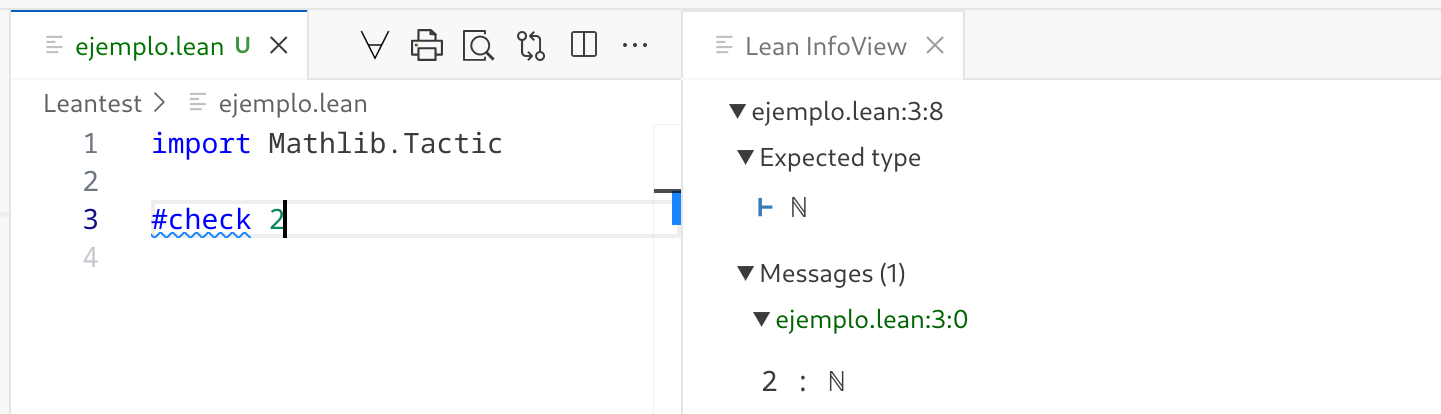
\includegraphics[width=1\textwidth]{figuras/check-example-light-version.png}
\end{figure}

En general, mientras escribimos en Lean, tendremos abierta esta ventana paralelamente a nuestro código, para poder ir viendo el progreso de nuestra demostración.

\newpage % la he puesto para que se viera la imagen en el sitio correcto

\begin{figure}[h]
  \centering
  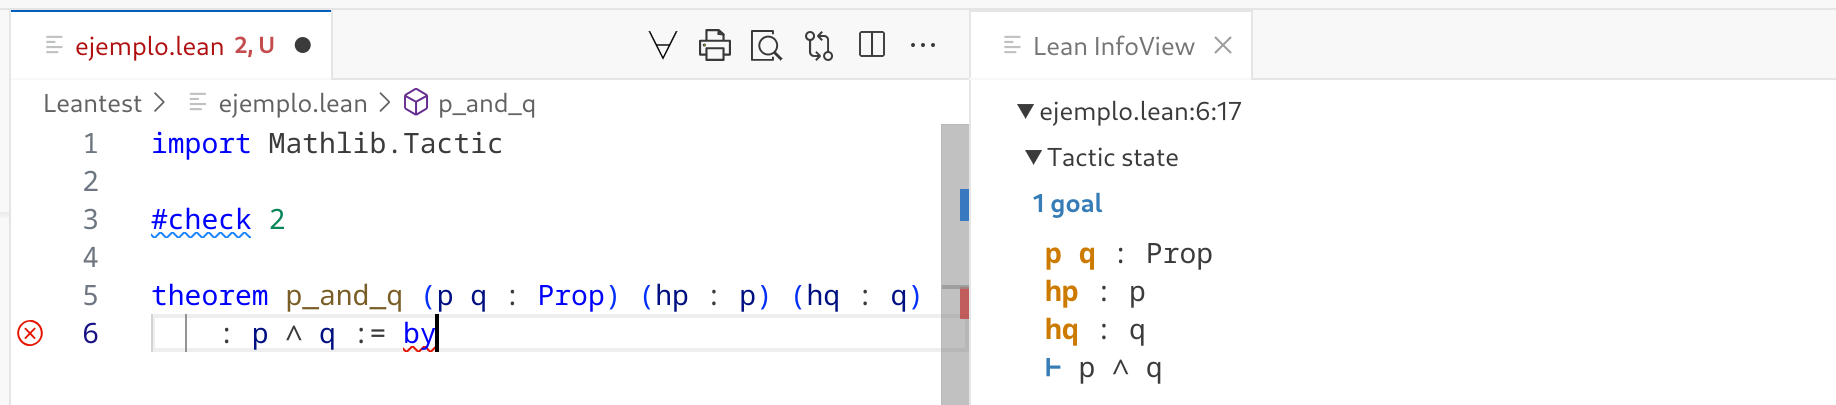
\includegraphics[width=1\textwidth]{figuras/theorem-example-light-version.png}
\end{figure}

Bajo el apartado \code{Tactic state}, podemos comprobar:

\begin{itemize}
  \item El número de tesis que nos quedan por demostrar (en este caso solo una: \bluecode{1 goal}).
  \item Nuestro contexto.
  \item La (o las) tesis, marcada con el símbolo \bluecode{$\vdash$}.
\end{itemize}

A partir de este punto, podemos empezar a añadir las tácticas que van a constituir nuestra demostración. Las tácticas se escriben una detrás de otra, separadas por punto y coma (\code{;}) o por saltos de línea.

Al escribir una táctica, el apartado \code{Tactic state} del InfoView se actualizará según corresponda. Cuando todas las tesis se hayan resuelto, el InfoView mostrará \bluecode{No goals}.

\begin{figure}[h]
  \centering
  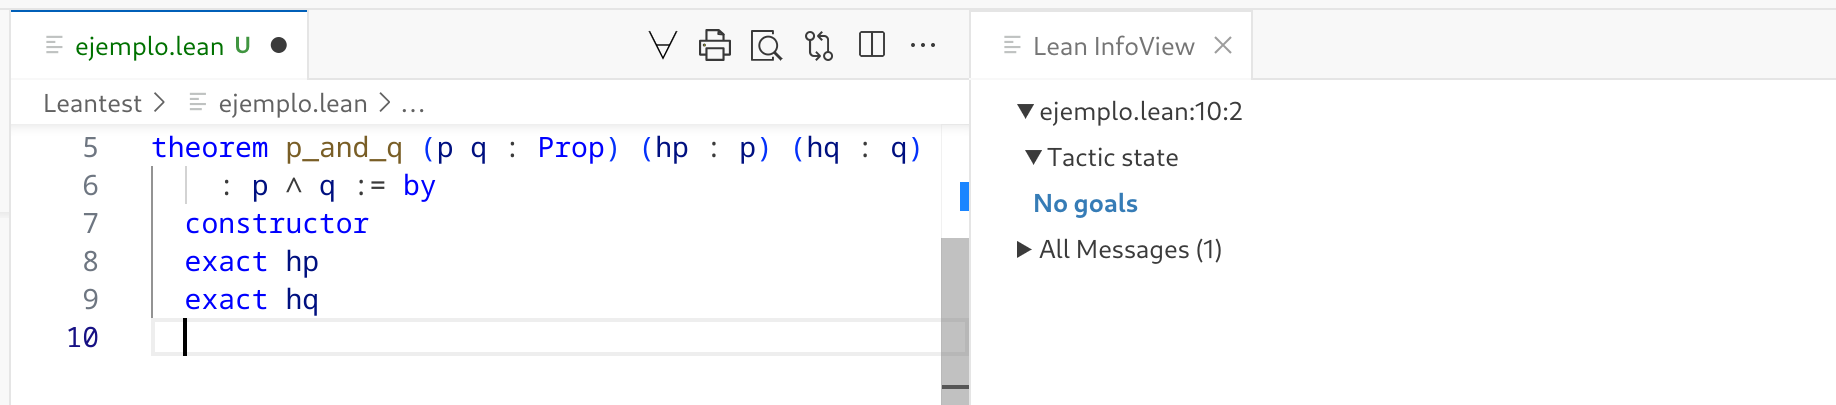
\includegraphics[width=1\textwidth]{figuras/no-goals-example-light-version.png}
\end{figure}

\subsubsection{Algunas tácticas básicas}

En esta sección veremos algunas de las tácticas más básicas y útiles para construir demostraciones en Lean. Veremos cómo se aplican y qué efecto tienen en el InfoView. El resto de tácticas que aparecen a lo largo del trabajo pueden consultarse en el Anexo (letra, probablemente la A).

Para poder utilizar las tácticas mencionadas a continuación, es necesario importar el módulo de Mathlib correspondiente al modo táctico mediante

\begin{lstlisting}
  import Mathlib.Tactic
\end{lstlisting}

A partir de aquí, en lugar de mostrar capturas del InfoView, utilizaremos dos bloques de código en paralelo: el de la izquierda contiene el código de Lean; el de la derecha representa el estado que se mostraría en el InfoView si colocásemos el cursor en la última línea.

\vspace{1em}
\noindent\textbf{$~$ \largebluecode{intro}}

La táctica \bluecode{intro} introduce un nuevo objeto en el contexto, de manera similar a escribir \quotes{Supongamos que...} o \quotes{Sea...} en una demostración informal.

Es útil cuando el objetivo tiene la forma de una implicación o un cuantificador universal: transformamos la primera parte de la tesis en una nueva hipótesis y la segunda en la nueva tesis. Por ejemplo, para la implicación:


\begin{minipage}[t]{0.58\textwidth}
\begin{lstlisting}[language=lean]
  example (p : Prop) : p → p := by


~
\end{lstlisting}
\end{minipage}%
\hfill
\begin{minipage}[t]{0.40\textwidth}
\begin{lstlisting}[language=infoview]
  Tactic state
    ŋ1 goalŋ
    ħpħ : Prop
    ⊢ p → p
\end{lstlisting}
\end{minipage}
%
\noindent
\makebox[\textwidth]{$\downarrow$}
%
\begin{minipage}[t]{0.58\textwidth}
\begin{lstlisting}[language=lean]
  example (p : Prop) : p → p := by
    intro hp


~
\end{lstlisting}
\end{minipage}%
\hfill
\begin{minipage}[t]{0.40\textwidth}
\begin{lstlisting}[language=infoview]
  Tactic state
    ŋ1 goalŋ
    ħpħ : Prop
    ħhpħ : p
    ⊢ p
\end{lstlisting}
\end{minipage}


Y para deshacer cuantificadores:

\begin{minipage}[t]{0.58\textwidth}
\begin{lstlisting}[language=lean]
  example : ∀ (p : Prop), p → p := by

~
\end{lstlisting}
\end{minipage}%
\hfill
\begin{minipage}[t]{0.40\textwidth}
\begin{lstlisting}[language=infoview]
  Tactic state
    ŋ1 goalŋ
    ⊢ ∀ (p : Prop), p → p
\end{lstlisting}
\end{minipage}
%
\noindent
\makebox[\textwidth]{$\downarrow$}
%
\begin{minipage}[t]{0.58\textwidth}
\begin{lstlisting}[language=lean]
  example : ∀ (p : Prop), p → p := by
    intro q

~
\end{lstlisting}
\end{minipage}%
\hfill
\begin{minipage}[t]{0.40\textwidth}
\begin{lstlisting}[language=infoview]
  Tactic state
    ŋ1 goalŋ
    ħqħ : Prop
    ⊢ q → q
\end{lstlisting}
\end{minipage}


\vspace{1em}
\noindent\textbf{$~$ \largebluecode{exact}}

La táctica \bluecode{exact} se utiliza cuando ya tenemos, en nuestro contexto, exactamente lo que queremos demostrar. Es decir, existe una hipótesis que coincide con la tesis actual. Por ejemplo:

\begin{minipage}[t]{0.58\textwidth}
\begin{lstlisting}[language=lean]
  example : ∀ (p : Prop), p → p := by
    intro p hp


~
\end{lstlisting}
\end{minipage}%
\hfill
\begin{minipage}[t]{0.40\textwidth}
\begin{lstlisting}[language=infoview]
  Tactic state
    ŋ1 goalŋ
    ħpħ : Prop
    ħhpħ : p
    ⊢ p
\end{lstlisting}
\end{minipage}
%
\noindent
\makebox[\textwidth]{$\downarrow$}
%
\begin{minipage}[t]{0.58\textwidth}
\begin{lstlisting}[language=lean]
  example : ∀ (p : Prop), p → p := by
    intro p hp
    exact hp
\end{lstlisting}
\end{minipage}%
\hfill
\begin{minipage}[t]{0.40\textwidth}
\begin{lstlisting}[language=infoview]
  Tactic state
    ŋNo goalsŋ
~
\end{lstlisting}
\end{minipage}


\vspace{1em}
\noindent\textbf{$~$ \largebluecode{apply}}

La táctica \bluecode{apply} nos permite usar una implicación para reducir un objetivo a otro más simple. Equivale a utilizar la regla del \textit{Modus Ponens}: si tenemos una hipótesis de la forma $p \rightarrow q$ y queremos demostrar $q$, basta con demostrar $p$.

\begin{minipage}[t]{0.58\textwidth}
\begin{lstlisting}[language=lean]
  example : (p q : Prop) (hp : p)
      (hpq : p → q) : q := by



~
\end{lstlisting}
\end{minipage}%
\hfill
\begin{minipage}[t]{0.40\textwidth}
\begin{lstlisting}[language=infoview]
  Tactic state
    ŋ1 goalŋ
    ħp qħ : Prop
    ħhpħ : p
    ħhpqħ : p → q
    ⊢ q
\end{lstlisting}
\end{minipage}
%
\noindent
\makebox[\textwidth]{$\downarrow$}
%
\begin{minipage}[t]{0.58\textwidth}
\begin{lstlisting}[language=lean]
  example : (p q : Prop) (hp : p)
      (hpq : p → q) : q := by
    apply hpq 


~
\end{lstlisting}
\end{minipage}%
\hfill
\begin{minipage}[t]{0.40\textwidth}
\begin{lstlisting}[language=infoview]
  Tactic state
    ŋ1 goalŋ
    ħp qħ : Prop
    ħhpħ : p
    ħhpqħ : p → q
    ⊢ p
\end{lstlisting}
\end{minipage}

Podríamos completar esta demostración usando \code{\blue{exact} hp}.


\vspace{1em}
\noindent\textbf{$~$ \largebluecode{use}}

Utilizamos \bluecode{use} para trabajar con el cuantificador existencial. Si queremos demostrar una proposición de la forma \quotes{$\exists x, P x$}, basta con encontrar un $x_0$ concreto que satisfaga la propiedad $P$.

En este caso, aplicamos \bluecode{use} para indicarle a Lean el valor concreto $x_0$ que queremos usar para demostrar la existencia. El objetivo pasa a ser entonces demostrar que $x_0$ satisface $P$. Por ejemplo:

\begin{minipage}[t]{0.58\textwidth}
\begin{lstlisting}[language=lean]
  example : ∃ n : ℕ, n > 3 := by

~
\end{lstlisting}
\end{minipage}%
\hfill
\begin{minipage}[t]{0.40\textwidth}
\begin{lstlisting}[language=infoview]
  Tactic state
    ŋ1 goalŋ
    ⊢ ∃ n, n > 3
\end{lstlisting}
\end{minipage}
%
\noindent
\makebox[\textwidth]{$\downarrow$}
%
\begin{minipage}[t]{0.58\textwidth}
\begin{lstlisting}[language=lean]
  example : ∃ n : ℕ, n > 3 := by
    use 5
~
\end{lstlisting}
\end{minipage}%
\hfill
\begin{minipage}[t]{0.40\textwidth}
\begin{lstlisting}[language=infoview]
  Tactic state
    ŋ1 goalŋ
    ⊢ 5 > 3
\end{lstlisting}
\end{minipage}


\vspace{1em}
\noindent\textbf{$~$ \largebluecode{left}, \largebluecode{right}}

Las tácticas \bluecode{left} y \bluecode{right} se utilizan para trabajar con disyunciones, es decir, proposiciones de la forma $A \lor B$.

En una demostración informal, si queremos demostrar que \quotes{$A$ o $B$} es cierto, nos basta con demostrar una de las dos. Utilizamos \bluecode{left} para indicar que vamos a demostrar la parte izquierda ($A$), y \bluecode{right} si queremos demostrar la parte derecha ($B$). Por ejemplo:

\begin{minipage}[t]{0.58\textwidth}
\begin{lstlisting}[language=lean]
  example : (p q : Prop) (hp : p) :
      p ∨ q := by


~
\end{lstlisting}
\end{minipage}%
\hfill
\begin{minipage}[t]{0.40\textwidth}
\begin{lstlisting}[language=infoview]
  Tactic state
    ŋ1 goalŋ
    ħp qħ : Prop
    ħhpħ : p
    ⊢ p ∨ q
\end{lstlisting}
\end{minipage}
%
\noindent
\makebox[\textwidth]{$\downarrow$}
%
\begin{minipage}[t]{0.58\textwidth}
\begin{lstlisting}[language=lean]
  example : (p q : Prop) (hp : p) :
      p ∨ q := by
    left

~
\end{lstlisting}
\end{minipage}%
\hfill
\begin{minipage}[t]{0.40\textwidth}
\begin{lstlisting}[language=infoview]
  Tactic state
    ŋ1 goalŋ
    ħp qħ : Prop
    ħhpħ : p
    ⊢ p
\end{lstlisting}
\end{minipage}

Podríamos completar esta demostración aplicando \code{\blue{exact} hp}.

\vspace{1em}
\noindent\textbf{$~$ \largebluecode{constructor}}

Utilizamos \bluecode{constructor} para trabajar con conjunciones, es decir, proposiciones de la forma $A \land B$.

Cuando queremos demostrar  que \quotes{$A$ y $B$} es cierto, podemos demostrar $A$ por un lado y $B$ por otro. Al aplicar \bluecode{constructor}, Lean divide un objetivo \code{A $\land$ B} en dos sub-objetivos con el mismo contexto: uno para \code{A} y otro para \code{B}. Por ejemplo:

\begin{minipage}[t]{0.58\textwidth}
\begin{lstlisting}[language=lean]
  example (p q : Prop) (hp : p)
      (hq : q) : p ∧ q := by



~
\end{lstlisting}
\end{minipage}%
\hfill
\begin{minipage}[t]{0.40\textwidth}
\begin{lstlisting}[language=infoview]
  Tactic state
    ŋ1 goalŋ
    ħp qħ : Prop
    ħhpħ : p
    ħhqħ : q
    ⊢ p ∧ q
\end{lstlisting}
\end{minipage}
%
\noindent
\makebox[\textwidth]{$\downarrow$}
%
\begin{minipage}[t]{0.58\textwidth}
\begin{lstlisting}[language=lean]
  example (p q : Prop) (hp : p)
      (hq : q) : p ∧ q := by
    constructor








~
\end{lstlisting}
\end{minipage}%
\hfill
\begin{minipage}[t]{0.40\textwidth}
\begin{lstlisting}[language=infoview]
  Tactic state
    ŋ2 goalsŋ
    case left
      ħp qħ : Prop
      ħhpħ : p
      ħhqħ : q
      ⊢ p
    case right
      ħp qħ : Prop
      ħhpħ : p
      ħhqħ : q
      ⊢ q
\end{lstlisting}
\end{minipage}

Después de aplicar \bluecode{constructor}, el InfoView mostrará dos objetivos pendientes (\bluecode{2 goals}). Al resolver cada uno por separado, completamos la demostración.

\begin{minipage}[t]{0.58\textwidth}
\begin{lstlisting}[language=lean]
  example (p q : Prop) (hp : p)
      (hq : q) : p ∧ q := by
    constructor
    exact hp
    exact hq
\end{lstlisting}
\end{minipage}%
\hfill
\begin{minipage}[t]{0.40\textwidth}
\begin{lstlisting}[language=infoview]
  Tactic state
    ŋNo goalsŋ


~
\end{lstlisting}
\end{minipage}

Aunque lo anterior es correcto, lo habitual cuando trabajamos con más de una tesis es utilizar \code{·} para separarlas. Cuando escribimos \code{·} tras un salto de línea, Lean enfoca el primer objetivo, ocultando temporalmente el resto. Por ejemplo:

\begin{minipage}[t]{0.58\textwidth}
\begin{lstlisting}[language=lean]
  example (p q : Prop) (hp : p)
      (hq : q) : p ∧ q := by
    constructor
    ·


~
\end{lstlisting}
\end{minipage}%
\hfill
\begin{minipage}[t]{0.40\textwidth}
\begin{lstlisting}[language=infoview]
  Tactic state
    ŋ1 goalŋ
    case left
      ħp qħ : Prop
      ħhpħ : p
      ħhqħ : q
      ⊢ p
\end{lstlisting}
\end{minipage}

Si colocamos el cursor al final, el InfoView solo muestra \bluecode{1 goal}, porque el segundo objetivo está oculto por ahora. La demostración completa en este estilo sería:


\begin{minipage}[t]{0.58\textwidth}
\begin{lstlisting}[language=lean]
  example (p q : Prop) (hp : p)
      (hq : q) : p ∧ q := by
    constructor
    · exact hp
    · exact hq
\end{lstlisting}
\end{minipage}%
\hfill
\begin{minipage}[t]{0.40\textwidth}
\begin{lstlisting}[language=infoview]
  Tactic state
    ŋNo goalsŋ


~
\end{lstlisting}
\end{minipage}


\vspace{1em}
\noindent\textbf{$~$ \largebluecode{cases'}}

La táctica \bluecode{cases'} se utiliza para analizar una disyunción en el contexto, es decir, una hipótesis de la forma $A \lor B$.

En una demostración informal, equivale a hacer un razonamiento por casos: \quotes{Supongamos que ocurre $A$, veamos si se sigue la tesis; supongamos depués que ocurre $B$, y comprobemos si también se sigue}.

Al aplicar \code{\blue{cases'} h } sobre una hipótesis h, Lean duplica el objetivo (que no cambia), pero modifica el contexto en cada uno de los nuevos objetivos, introduciendo las hipótesis correspondientes a cada caso. Utilizamos el comando \bluecode{with} para asignar nombres a las nuevas hipótesis. Por ejemplo:

\begin{minipage}[t]{0.58\textwidth}
\begin{lstlisting}[language=lean]
  example (p q : Prop) (h : p ∨ q)
      (hpq : p → q) : q := by



~
\end{lstlisting}
\end{minipage}%
\hfill
\begin{minipage}[t]{0.40\textwidth}
\begin{lstlisting}[language=infoview]
  Tactic state
    ŋ1 goalŋ
    ħp qħ : Prop
    ħhħ : p ∨ q
    ħhpqħ : p → q
    ⊢ q
\end{lstlisting}
\end{minipage}
%
\noindent
\makebox[\textwidth]{$\downarrow$}
%
\begin{minipage}[t]{0.58\textwidth}
\begin{lstlisting}[language=lean]
  example (p q : Prop) (h : p ∨ q)
      (hpq : p → q) : q := by
    cases' h with hp hq







      
~
\end{lstlisting}
\end{minipage}%
\hfill
\begin{minipage}[t]{0.40\textwidth}
\begin{lstlisting}[language=infoview]
  Tactic state
    ŋ2 goalsŋ
    case inl
      ħp qħ : Prop
      ħhpqħ : p → q
      ħhpħ : p
      ⊢ q
    case inr
      ħp qħ : Prop
      ħhpqħ : p → q
      ħhqħ : q
      ⊢ q
\end{lstlisting}
\end{minipage}

Podemos entonces completar la demostración con las herramientas que tenemos hasta ahora:

\begin{minipage}[t]{0.58\textwidth}
\begin{lstlisting}[language=lean]
  example (p q : Prop) (h : p ∨ q)
      (hpq : p → q) : q := by
    cases' h with hp hq
    · apply hpq
      exact hp
    · exact hq
\end{lstlisting}
\end{minipage}%
\hfill
\begin{minipage}[t]{0.40\textwidth}
\begin{lstlisting}[language=infoview]
  Tactic state
    ŋNo goalsŋ



~
\end{lstlisting}
\end{minipage}


Como hemos visto por medio de estos ejemplos, completar una demostración en modo táctico consiste en combinar estas instrucciones una después de otra, haciendo que las hipótesis y las tesis vayan avanzando hasta alcanzar el estado deseado: \bluecode{No goals}. Las tácticas nos dan la flexibilidad necesaria para formalizar una gran variedad de resultados matemáticos.



\subsubsection{Herramientas de automatización y búsqueda en Mathlib}

A medida que las demostraciones en Lean se vuelven más complejas, no siempre resulta práctico construir cada paso manualmente. Para agilizar el proceso, Lean incorpora algunas herramientas de automatización que permiten delegar ciertas tareas al sistema.

Además, en lugar de volver a demostrar resultados que ya están formalizados, es fundamental \textbf{aprovechar la biblioteca matemática de Lean, Mathlib}, que contiene miles de definiciones y teoremas disponibles para su reutilización.

Sin embargo, apoyarse en Mathlib no siempre es directo: los resultados pueden tener nombres poco intuitivos o muy específicos, y encontrar el lema que necesitamos en un momento dado no es siempre fácil.

Por ejemplo, un resultado tan simple como: \quotes{Si $a, b, c$ son números reales tales que $a < b$ y $c < 0$, entonces $a + c < b$} (que en una prueba informal consideraríamos casi trivial), aparece en Mathlib con el nombre \code{add\_lt\_of\_lt\_of\_neg'}. En la práctica, recordar todos estos nombres resulta inviable, incluso para resultados elementales.

En esta sección introduciremos las tácticas \bluecode{simp} y \bluecode{exact?}, que nos ayudan a resolver objetivos simples, y dos herramientas externas que podemos utilizar para localizar resultados en Mathlib. Además, veremos la forma en la que integrar estas herramientas en nuestro proceso de demostración de resultados.

\vspace{1em}
\noindent\textbf{$~$ \largebluecode{simp}}

La manera más sencilla de apoyarse en la librería de Mathlib es utilizar la táctica \bluecode{simp}. Esta táctica hace una búsqueda exhaustiva entre una base de datos de lemas de Mathlib que están marcados con el atributo \code{simp}, intentando simplificar lo máximo posible el objetivo o las hipótesis a las que se aplique.

La táctica \bluecode{simp} se puede utilizar en cualquier momento de la demostración, pero resulta especialmente útil cuando algo que queremos demostrar parece evidente o suficientemente simple. Por ejemplo:

\begin{lstlisting}
  example (G : Type) [Group G] (a b c : G) :
      a * a⁻¹ * 1 * b = b * c * c⁻¹ := by
   simp
\end{lstlisting}

Solamente usando \bluecode{simp} podemos terminar la demostración en este caso. Realmente, lo único que hace es reescribir reiteradamente resultados de la forma \code{A = B} ó \code{A $\leftrightarrow$ B}, hasta que no puede reescribir nada más, de manera mecánica. Por tanto, aunque es útil en muchos casos, en otros es posible que no nos ayude.

En la práctica, cuando nos resulte sencillo utilizar otras tácticas o resultados conocidos, eso será preferible a utilizar \bluecode{simp}, primero porque al tratarse de una búsqueda exhaustiva, no es una táctica computacionalmente eficiente, y segundo porque empeora la legibilidad del código, ya que a veces es difícil saber cómo ocurren ciertas simplificaciones.

\vspace{1em}
\noindent\textbf{$~$ \largebluecode{exact?}}

Lean incorpora algunas tácticas que intentan cerrar el objetivo actual utilizando tanto las hipótesis del contexto como los resultados disponibles en los archivos importados. Las más destacadas son \bluecode{exact?}\footnote{La táctica \bluecode{exact?} tenía el nombre \bluecode{library\_search} en Lean 3.} y \bluecode{apply?}.

A lo largo del proyecto, la que he utilizado con mayor frecuencia es \bluecode{exact?}. Esta táctica intenta encontrar una expresión que tenga exactamente el tipo del objetivo actual, buscando tanto en la información local (hipótesis del contexto, resultados definidos anteriormente) como en la librería de Mathlib.

Por ejemplo, en el caso de encontrar hipótesis locales:

\begin{minipage}[t]{0.58\textwidth}
\begin{lstlisting}[language=lean]
  example (p : Prop) : p → p := by
    intro hp
    exact?
\end{lstlisting}
\end{minipage}%
\hfill
\begin{minipage}[t]{0.40\textwidth}
\begin{lstlisting}[language=infoview]
  Suggestions
    Try this: exact hp
~
\end{lstlisting}
\end{minipage}

Y en el caso de encontrar resultados de Mathlib:

\begin{minipage}[t]{0.58\textwidth}
\begin{lstlisting}[language=lean]
  example (n : ℕ) : n ≥ 0 := by
	  exact?
  ~
\end{lstlisting}
\end{minipage}%
\hfill
\begin{minipage}[t]{0.40\textwidth}
\begin{lstlisting}[language=infoview]
  Suggestions
    Try this: exact Nat.zero_le n
\end{lstlisting}
\end{minipage}

En general, utilizar la expresión sugerida por \bluecode{exact?} concluirá la prueba.

A pesar de que \bluecode{exact?} nos puede ayudar en muchos casos, es una herramienta relativamente sencilla, que solo puede dar un paso (aplicar un teorema o una hipótesis). Esto implica que si no tenemos las hipótesis exactas de los teoremas como aparecen en Mathlib, \bluecode{exact?} no encontrará ninguna solución.

Cuando trabajamos con hipótesis más complejas, lo habitual no es utilizar \bluecode{exact?} directamente para probar nuestra tesis, sino para probar ciertos resultados intermedios. Por esto, una táctica crucial a la hora de trabajar con \bluecode{exact?} es \bluecode{have}, el equivalente en demostraciones informales a declarar un lema en mitad de una demostración. Por ejemplo, supongamos que queremos probar:


\begin{lstlisting}
  example (p q r : Prop) (hpq : p → q) (hqr : q → r) (hp : p) : r
\end{lstlisting}

En lugar de tratar de demostrar inmediatamente \code{r}, podríamos probar, de manera intermedia, que se tiene \code{q}. Para esto utilizamos \bluecode{have}:

\begin{minipage}[t]{0.58\textwidth}
\begin{lstlisting}[language=lean]
  example (p q r : Prop) (hpq : p → q)
      (hqr : q → r) (hp : p) : r := by
    have hq : q



~
\end{lstlisting}
\end{minipage}%
\hfill
\begin{minipage}[t]{0.40\textwidth}
\begin{lstlisting}[language=infoview]
  Tactic state
    ŋ2 goalsŋ
    case hq
      ħ(...)ħ
      ⊢ q
    ħ(...)ħ
    ⊢ r
\end{lstlisting}
\end{minipage}

Escribir \code{\blue{have} hq : q} introduce una nueva tesis, \code{q}, independiente de la anterior. Una vez completemos la prueba de esta nueva tesis, podremos usar el resultado en nuestra demostración. Por tanto, podríamos completar el ejemplo anterior de la siguiente forma:

\begin{lstlisting}
  example (p q r : Prop) (hpq : p → q) (hqr : q → r) (hp : p) : r := by
    have hq : q
    · apply hpq
      exact hp
    apply hqr
    exact hq
\end{lstlisting}

Recordemos que utilizamos el punto \code{·} para separar la demostración de \code{hq} del resto de la demostración.

Veamos por tanto como es el proceso de trabajar con \bluecode{exact?}. Consideremos el siguiente ejemplo, para el que \bluecode{exact?} no encuentra ningún resultado:


\begin{minipage}[t]{0.58\textwidth}
\begin{lstlisting}[language=lean]
  example (x : ℝ) (hx : x > 0) :
      x / x = 1 := by
    exact?




~
\end{lstlisting}
\end{minipage}%
\hfill
\begin{minipage}[t]{0.40\textwidth}
\begin{lstlisting}[language=infoview]
  Tactic state
    ŋ1 goalŋ
    ħxħ : ℝ
    ħhxħ : x > 0
    ⊢ x / x = 1
  Messages
    `exact?` could not close the goal.
\end{lstlisting}
\end{minipage}

\begin{enumerate}
  \item Mirando el estado actual de la demostración, identificar cuál sería una hipótesis que desearíamos tener en nuestro contexto. En este caso, al tratarse de una división, podría ser necesario tener la hipótesis $x \neq 0$.
  \item Añadir la nueva tesis utilizando \blue{have}\footnote{En algunos casos, será más útil escribir aquello que creemos poder necesitar fuera de la demostración, utilizando \bluecode{example}, porque podremos escribir resultados más generales.}.
\end{enumerate}

\vspace{-1.5em}
\begin{minipage}[t]{0.58\textwidth}
\begin{lstlisting}[language=lean]
  example (x : ℝ) (hx : x > 0) :
      x / x = 1 := by
    have h : x ≠ 0
    · 
~
\end{lstlisting}
\end{minipage}%
\hfill
\begin{minipage}[t]{0.40\textwidth}
\begin{lstlisting}[language=infoview]
  Tactic state
    ŋ1 goalŋ
    ħxħ : ℝ
    ħhxħ : x > 0
    ⊢ x ≠ 0
\end{lstlisting}
\end{minipage}
\vspace{-1.5em}

\begin{enumerate}
  \setcounter{enumi}{2}
  \item Intentar demostrar la nueva tesis utilizando \bluecode{exact?}.
\end{enumerate}

\vspace{-1.5em}
\begin{minipage}[t]{0.58\textwidth}
\begin{lstlisting}[language=lean]
  example (x : ℝ) (hx : x > 0) :
      x / x = 1 := by
    have h : x ≠ 0
    · exact?
\end{lstlisting}
\end{minipage}%
\hfill
\begin{minipage}[t]{0.40\textwidth}
\begin{lstlisting}[language=infoview]
  Suggestions
    Try this: Ne.symm (ne_of_lt hx)
~
\end{lstlisting}
\end{minipage}


Con esta nueva hipótesis, parece probable que \bluecode{exact?} sea capaz de terminar la demostración. En efecto:

\begin{minipage}[t]{0.58\textwidth}
\begin{lstlisting}[language=lean]
  example (x : ℝ) (hx : x > 0) :
      x / x = 1 := by
    have h : x ≠ 0
    · exact Ne.symm (ne_of_lt hx)
    exact?
\end{lstlisting}
\end{minipage}%
\hfill
\begin{minipage}[t]{0.40\textwidth}
\begin{lstlisting}[language=infoview]
  Suggestions
    Try this: (div_eq_one_iff_eq h).mpr rfl
~
\end{lstlisting}
\end{minipage}

La táctica \bluecode{exact?} es un ejemplo de motor de búsqueda formal: una herramienta que, mediante meta-programación en Lean, compara el objetivo actual con los tipos de todos los lemas disponibles y devuelve aquellos con coincidencias exactas. Por tanto, la clave de usar \bluecode{exact?} de manera eficaz reside en \textbf{desarrollar gradualmente una cierta intuición} sobre qué resultados es probable que estén formalizados en Mathlib, y la forma concreta en la que están formulados.

En efecto, reconocer que un lema de Mathlib sobre división por $x$ probablemente requería la hipótesis $x\neq0$ (y no simplemente $x>0$) ha sido esencial para poder aplicar \bluecode{exact?} con éxito en el ejemplo anterior.

A parte de \bluecode{exact?}, existen tácticas similares como \bluecode{apply?} y \bluecode{rw?}, que funcionan del mismo modo y permiten dar pasos intermedios. Sin embargo, en la práctica estas tácticas suelen devolver una larga lista de opciones, muchas de las cuales no son relevantes o útiles. Por tanto, cuando \bluecode{exact?} no es suficiente, es más eficaz recurrir a otras herramientas de búsqueda.


\vspace{1em}
\noindent\textbf{$~$ Otras herramientas}

A lo largo de este proyecto he utilizado fundamentalmente dos herramientas externas de búsqueda en Mathlib: Moogle \cite{moogle} y LeanSearch \cite{gao2024semantic}. Ambos son motores de búsqueda semántica, lo que significa que no se limitan a buscar coincidencias literales en el texto, sino que intentan interpretar el significado matemático de nuestra consulta y compararlo con los resultados de Mathlib. Para ello utilizan modelos de lenguaje de gran escala (LLMs), que permiten establecer relaciones entre enunciados aunque estén formulados de distinta manera. En particular, admiten consultas con los siguientes formatos \cite{gao2024semantic}:

\begin{itemize}
  \item Descripciones en lenguaje natural
  \item Nombres de teoremas conocidos
  \item Notación matemática (en LaTeX)
  \item Código Lean
\end{itemize}

Por ejemplo, si en el caso anterior no se nos hubiera ocurrido la idea de demostrar primero $x \neq 0$, podríamos haber buscado en Moogle algo del estilo de \textit{\quotes{division by itself is 1}}. De hecho, el segundo resultado de esta búsqueda en Moogle es:

\begin{figure}[h]
  \centering
  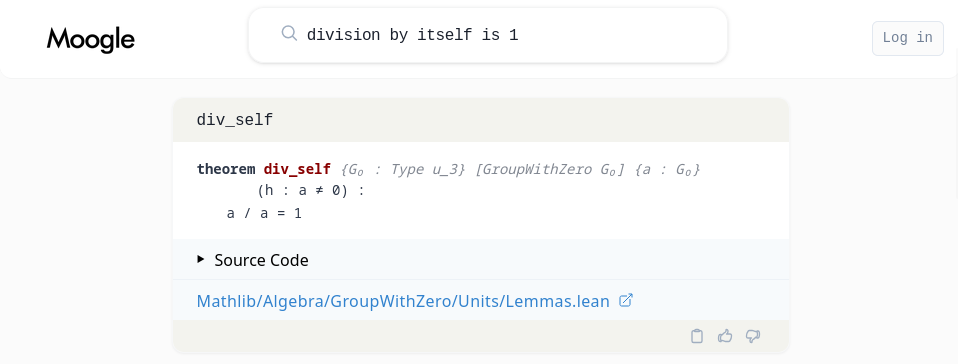
\includegraphics[width=1\textwidth]{figuras/moogle-example.png}
\end{figure}

Que no es el mismo resultado que proponía \bluecode{exact?}, pero parece incluso más simple. Podríamos volver a nuestro ejemplo y escribir

\begin{minipage}[t]{0.58\textwidth}
\begin{lstlisting}[language=lean]
  example (x : ℝ) (hx : x > 0) :
      x / x = 1 := by
    apply div_self

~
\end{lstlisting}
\end{minipage}%
\hfill
\begin{minipage}[t]{0.40\textwidth}
\begin{lstlisting}[language=infoview]
  Tactic state
    ŋ1 goalŋ
    ħxħ : ℝ
    ħhxħ : x > 0
    ⊢ x ≠ 0
\end{lstlisting}
\end{minipage}

Con lo que ya sólo faltaría demostrar que $x \neq 0$.

En general, he encontrado que LeanSearch funciona mejor que Moogle, especialmente en términos de relevancia de los resultados obtenidos. Sin embargo, al principio del proyecto solo conocía Moogle, y descubrí LeanSearch más tarde, por lo que he utilizado Moogle mayoritariamente.

Un ejemplo de una búsqueda real que necesité para el trabajo en LeanSearch, fue \textit{\quotes{subset of set has at most the dimension of the set}}.

\begin{figure}[h]
  \centering
  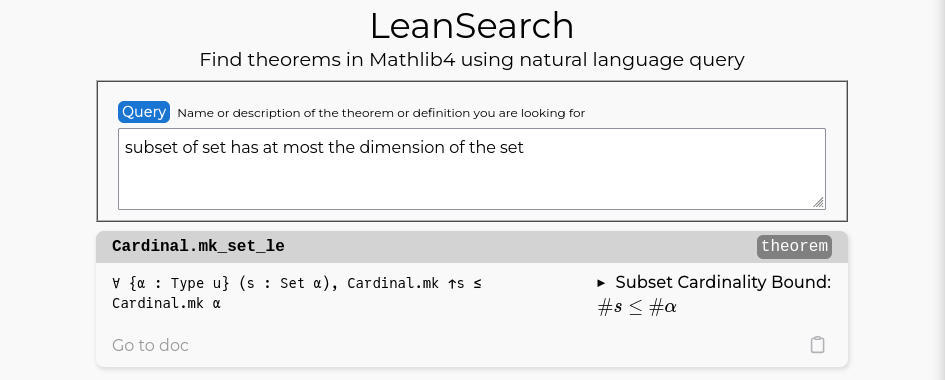
\includegraphics[width=1\textwidth]{figuras/leansearch-example-cropped.png}
\end{figure}

El primer resultado que aparece es justo el que necesitaba. Sin embargo, antes de buscarlo no tenía ninguna idea de cómo formalizar los resultados en los que estaba trabajando, especialmente porque no estaba familiarizada con el módulo \code{Cardinal}. Este fue un ejemplo claro de que estas herramientas permiten acceder a partes de Mathlib que de otro modo serían difíciles de localizar.

En conjunto, herramientas como \bluecode{exact?}, LeanSearch o Moogle han resultado fundamentales para hacer más eficiente el proceso de formalización, permitiendo apoyarse en Mathlib de forma efectiva sin necesidad de conocerla en profundidad desde el principio.


\subsubsection{Noncomputable y el axioma de elección}

Para finalizar esta sección sobre Lean en la práctica, es útil comentar brevemente una cuestión que aparecerá en algunas de las definiciones posteriores: el uso del \textbf{axioma de elección} y la palabra clave \bluecode{noncomputable}.

En Lean, el axioma de elección se introduce de la siguiente forma:

\begin{lstlisting}
  axiom choice {α : Sort u} : Nonempty α → α
\end{lstlisting}

Es decir, dado un tipo no vacío, \code{choice} devuelve un elemento de ese tipo, aunque no nos dice cómo encontrarlo. Por este motivo, su uso impide extraer información computable del resultado.

En consecuencia, cuando definimos funciones o construcciones que dependen de \code{choice}, Lean nos obliga a marcarlas como \bluecode{noncomputable}.  Un ejemplo es la función \code{choose}, que dada una prueba de tipo existencial, selecciona un testigo:

\begin{lstlisting}
  noncomputable def choose {α : Sort u} {p : α → Prop}
      (h : ∃ x, p x) : α :=
    (indefiniteDescription p h).val
\end{lstlisting}

A menudo utilizaremos \code{choose} (\code{Classical.choose}, ya que se encuentra en el módulo \code{Classical}) en nuestros resultados, junto con el siguiente lema

\begin{lstlisting}
  theorem choose_spec {α : Sort u} {p : α → Prop}
      (h : ∃ x, p x) : p (choose h) :=
    (indefiniteDescription p h).property
\end{lstlisting}

que es una demostración de que el elemento elegido mediante \code{choose} cumple las propiedades que le pedíamos.

El uso de \bluecode{noncomputable} no representa un problema para nosotros (ni, en general, para la comunidad matemática), ya que en este trabajo no nos interesa que las construcciones sean computables: trabajamos con ellas desde un punto de vista lógico y matemático, no algorítmico.

Además, usar el axioma de elección tiene una ventaja práctica: cuando utilicemos \code{choose}, el elemento elegido será siempre el mismo (aunque no sepamos cuál es), y tendrá siempre la propiedad \code{choose\_spec}. Esto permite trabajar con él de forma coherente dentro de una demostración y referirse a él varias veces como si fuera un objeto determinado.

En contraposición, otra forma de obtener un testigo de una prueba de existencia es utilizar la táctica \bluecode{obtain}, que se utiliza de la siguiente manera:

\begin{lstlisting}
  example : (∃ n : ℕ, n > 3) → ∃ m : ℕ, m > 2 := by
  intro h   -- h : ∃ n : ℕ, n > 3
  obtain ⟨n, hn⟩ := h    -- n : ℕ, hn : n > 3
  ...
\end{lstlisting}

La diferencia fundamental entre utilizar el axioma de elección y utilizar \bluecode{obtain} es que dos testigos obtenidos mediante obtain del mismo tipo (por ejemplo de tipo \code{$\exists$ n : $nat$, n > 3}) no serán necesariamente iguales, mientras que si fueron obtenidos mediante \code{Classical.choose} siempre serán iguales.

\newpage

\section{Espacios topológicos en Lean}

Explicar algunos ejemplos de definiciones y demostraciones, no a modo de explicación completa de los prerrequisitos de topología sino para tener un primer acercamiento sencillo a la topología en Lean.

Nota: toda esta sección se basa en el Willard en principio (para la teoría). \cite{willard2012general}

\subsection{Espacios topológicos}

\begin{definition}[\textbf{Espacio topológico}]\label{def:espacio-topologico}
    Sea $X$ un conjunto y $\mathcal{T}$ una colección de subconjuntos de $X$ de forma que
    \begin{enumerate}
      \item Los conjuntos $\emptyset$ y $X$ pertenecen a $\mathcal{T}$.
      \item Cualquier intersección finita de elementos de $\mathcal{T}$ pertenece a $\mathcal{T}$.
      \item Cualquier unión arbitraria de elementos de $\mathcal{T}$ pertenece a $\mathcal{T}$.
    \end{enumerate}
    Entonces diremos que $\mathcal{T}$ es una \textnormal{topología} sobre $X$, que $(X, \mathcal{T})$ es un \textnormal{espacio topológico} y que los elementos de $\mathcal{T}$ son \textnormal{abiertos} en este espacio.
\end{definition}

En Lean, esta definición se escribe como una estructura que consta de cuatro elementos:

\begin{lstlisting}
  class TopologicalSpace (X : Type u) where
    IsOpen : Set X → Prop
    isOpen_univ : IsOpen Set.univ
    isOpen_inter : ∀ s t, IsOpen s → IsOpen t → IsOpen (s ∩ t)
    isOpen_sUnion : ∀ s, (∀ t ∈ s, IsOpen t) → IsOpen (⋃₀ s)
\end{lstlisting}

El primer elemento, \code{IsOpen}, es una función que lleva cada conjunto de $X$ en una proposición, es decir, es una descripción de los elementos de $\mathcal{T}$ como el conjunto \code{\{U $\in$ Set (X) | IsOpen U\}}. Los otros tres elementos son demostraciones de las propiedades de la definición.

Veamos algunos ejemplos y sus demostraciones en Lean.

\begin{example}\label{ex:topologia-discreta}
    Sea $X$ un conjunto cualquiera. Consideremos la colección $\mathcal{T}$ de todos los subconjuntos de $\mathcal{T}$. Entonces $\mathcal{T}$ es una topología sobre $X$, a la que llamamos \textnormal{topología discreta}.
\end{example}

\begin{proof}
  Podemos describir $\mathcal T$ como \code{\{U $\in$ Set (X) | True\}}, porque \code{IsOpen} es cierto para cualquier $U$.

  \begin{lstlisting}
  def DiscreteTopo (X : Type) : TopologicalSpace X where
    IsOpen (_ : Set X) := true \end{lstlisting}
  
  Ahora, demostrar el resto de propiedades es sencillo:

  \begin{minipage}[t]{0.58\textwidth}
\begin{lstlisting}[language=lean]
    isOpen_univ := by
  ~
\end{lstlisting}
\end{minipage}%
\hfill
\begin{minipage}[t]{0.40\textwidth}
\begin{lstlisting}[language=infoview]
  ⊢ (fun x ↦ true = true) Set.univ
\end{lstlisting}
\end{minipage}

Aplicar la función \code{fun x $\mapsto$ true} a cualquier conjunto retorna siempre \code{true}, por tanto basta con usar \bluecode{trivial}.

\begin{lstlisting}
  def DiscreteTopo (X : Type) : TopologicalSpace X where
    IsOpen (_ : Set X) := true
    isOpen_univ := by
      trivial
    isOpen_inter := by
      intros
      trivial
    isOpen_sUnion := by
      intros
      trivial
\end{lstlisting}

\end{proof}


\begin{example}\label{ex:topologia-trivial}
    Sea $X$ un conjunto cualquiera. Consideremos la colección $\mathcal{T}=\{\emptyset, X\}$. Entonces $\mathcal{T}$ es una topología sobre $X$, a la que llamamos \textnormal{topología trivial}.
\end{example}

\begin{proof}
  Podemos describir $\mathcal{T}$ como \code{\{U $\in$ Set (X) | U = X $\lor$ U = $\emptyset$\}}.

  \begin{lstlisting}
  def TrivialTopology (X : Type) : TopologicalSpace X where
    IsOpen (s : Set X) := s = Set.univ ∨ s = ∅ \end{lstlisting}

  La primera condición se cumple trivialmente: queremos ver $X = X \lor X = \emptyset$.

  \begin{lstlisting}
    isOpen_univ := by
      left
      rfl\end{lstlisting}

  Consideremos ahora dos abiertos (\bluecode{intro}). Diferenciamos en casos:

  \begin{lstlisting}
    isOpen_inter := by
      intro s t hs ht
      cases' hs with hs_univ hs_empty
      cases' ht with ht_univ ht_empty \end{lstlisting}

  Si ambos son $X$, la intersección será $X$ y por tanto abierta. Si uno de los dos es vacío, entonces la intersección es vacía, también abierta.

  \begin{lstlisting}
      · left -- s, t = Set.univ, s ∩ t = Set.univ ?
        rw [hs_univ, ht_univ]
        simp
      · right -- t = ∅, s ∩ t = ∅ ?
        rw [ht_empty]
        simp
      · right -- s = ∅, s ∩ t = ∅ ?
        rw [hs_empty]
        simp \end{lstlisting}

  Consideremos finalmente una colección arbitraria $S$ de abiertos. Para ver si la unión es abierta, consideramos dos casos distintos: o bien $X$ está en $S$, en cuyo caso la unión en $X$, o bien no lo está, en cuyo caso todos los conjuntos son vacíos y la unión también lo es.

  \begin{lstlisting}
    isOpen_sUnion := by
      intro S hS
      cases' Classical.em (Set.univ ∈ S) with h1 h2

      · left -- h1 : Set.univ ∈ S, ⋃₀S = Set.univ ?
        ext s
        constructor
        · intro hs -- hs : s ∈ S, s ∈ Set.univ ?
          trivial
        · intro hs -- hs : s ∈ Set.univ, s ∈ S ?
          use Set.univ -- utiliza h1 implicitamente

      · right -- h2 : Set.univ ∉ S, ⋃₀S = ∅ ?
        simp -- ∀ s ∈ S, s = ∅ ?
        intro s hs
        specialize hS s hs -- aplicar definicion de abierto
        cases' hS with hS hS -- dividir en casos
        · by_contra -- si s = Set.univ, contradiccion
          rw [hS] at hs 
          exact h2 hs -- porque s ∈ S, pero Set.univ ∉ S
        · exact hS -- si s = ∅ \end{lstlisting}
\end{proof}


\begin{example}

  Consideremos la recta real y consideremos la definición usual de conjunto abierto en $\mathbb{R}$, es decir, $A \subseteq \mathbb{R}$ es abierto si y solo si para cada punto $x \in A$ existe una bola abierta centrada en $x$ enteramente contenida en $A$. Sea $\mathcal{T}$ la colección de estos abiertos. Entonces $\mathcal{T}$ es una topología sobre $\mathbb{R}^2$, a la que llamamos \textnormal{topología usual}.
\end{example}

\begin{proof}
  En Lean, podemos describir este espacio topológico dando sus elementos de la siguiente forma, donde cada objeto esta definido anteriormente.

  
  \begin{lstlisting}
  def UsualTopology : TopologicalSpace ℝ where
    IsOpen := Real.IsOpen
    isOpen_univ := Real.isOpen_univ
    isOpen_inter := Real.isOpen_inter
    isOpen_sUnion := Real.isOpen_sUnion \end{lstlisting}
  
  La definición de abierto se puede escribir así:

  \begin{lstlisting}
  def Real.IsOpen (s : Set ℝ) : Prop :=
    ∀ x ∈ s, ∃ δ > 0, ∀ y : ℝ, x - δ < y ∧ y < x + δ → y ∈ s \end{lstlisting}

  Damos la demostración para la intersección finita. El resto utilizan mecanismos parecidos.

  Sean por tanto dos subconjuntos $s$ y $t$ de $\mathcal{T}$. Sea $x \in t \cap s$ y queremos ver que existe una bola abierta centrada en $x$ y contenida en $t \cap s$.

  \begin{lstlisting}
  lemma Real.isOpen_inter (s t : Set ℝ)
      (hs : IsOpen s) (ht : IsOpen t) : IsOpen (s ∩ t) := by
    intro x hx -- x ∈ s ∩ t, ∃ δ > 0, ∀ (y : ℝ), ... → y ∈ s ∩ t ? \end{lstlisting}

  Puesto que $x \in s$, existe un $\delta_1>0$ (\code{h$\delta$1}) de forma que $B_{\delta_1}(x) \subseteq s$ (\code{hs}). Análogamente, existe un $\delta_2>0$ (\code{h$\delta$2}) de forma que $B_{\delta_2}(x) \subseteq t$ (\code{ht}). Basta con tomar $\delta = \min \{\delta_1, \delta_2\}$.

  \begin{lstlisting}
    obtain ⟨δ1, hδ1, hs⟩ := hs x hx.left
    obtain ⟨δ2, hδ2, ht⟩ := ht x hx.right
    use min δ1 δ2 \end{lstlisting}

  Trivialmente $\delta > 0$.
  
  \begin{lstlisting}
    constructor
    · exact lt_min hδ1 hδ2 \end{lstlisting}

  Para ver que $B_\delta (x) \subseteq s \cap t$, consideramos $y \in B_\delta(x)$ y queremos ver que $y \in s$ y que $y \in t$. Para ver $y \in s$, como $B_{\delta_1}(x) \subseteq s$ (\code{hs}), basta ver $y \in B_{\delta_1}(x)$.

  \begin{lstlisting}
    · intro y hy
      constructor
      · apply hs -- x - δ1 < y ∧ y < x + δ1 ? \end{lstlisting}

  En realidad, esta condición se reduce a dos inecuaciones, que son fáciles de probar contando con que $\delta \leq \delta_1$ (\code{h$\delta$}).

  \begin{lstlisting}
      have hδ := min_le_left δ1 δ2
      constructor
      all_goals linarith \end{lstlisting}

  Probar que $y \in t$ es análogo.
  
\end{proof}


\subsubsection{Conjuntos abiertos}

Como hemos dicho, los conjuntos abiertos en un espacio topológico son los elementos de la topología. En Lean, es una función \code{TopologicalSpace.IsOpen} de tipo \code{Set X $\to$ \blue{Prop}}. Podemos utilizar esta definición directamente para demostrar que un abierto lo es.

\begin{example} 
    Por ejemplo, por definición, el universo, $X$, siempre es abierto. En efecto:
\end{example}

\begin{lstlisting}
  example (X : Type) [T : TopologicalSpace X] : T.IsOpen Set.univ := by
    exact TopologicalSpace.isOpen_univ \end{lstlisting}

\begin{example}
  En la Definición \ref{def:espacio-topologico}, requeríamos que el vacío es abierto. Sin embargo, en la definición de Mathlib no hemos pedido la misma condición.

  Se puede probar que el vacío es abierto a partir del resto de condiciones: podemos escribir $\emptyset$ como $\emptyset = \bigcup_{x \in \emptyset} \{x\}$. Aplicando que la unión arbitraria de abiertos es abierta, bastaría ver que $\forall x \in \emptyset$, $\{x\}$ es un conjunto abierto. Lo cual es trivial.
\end{example}

\begin{lstlisting}
  example {X : Type} [T : TopologicalSpace X] :
      IsOpen (∅ : Set X) := by
    rw [← Set.sUnion_empty] -- ∅ = ⋃₀ ∅
    apply isOpen_sUnion
    intro t ht -- ∀ t ∈ ∅, IsOpen t ?
    exfalso
    exact ht -- t ∈ ∅ = False
\end{lstlisting}
  
\begin{example}\label{ejemplo:intervalos-abiertos}
  En la topología usual, $(\mathbb{R}, \mathcal{T}_u)$, los intervalos abiertos $I = (a, b)$ con $a < b$ son abiertos.
\end{example}

\begin{proof}
  Consideremos un intervalo de la forma $(a, b)$ y queremos ver que es abierto. Para ello, sea $x \in (a, b)$, y veamos que existe un $\delta >0$ tal que $\forall y \in \mathbb{R}$, si $y \in B_\delta(x)$ entonces $y \in (a, b)$.

  \begin{lstlisting}
  lemma ioo_open_in_R (a b : ℝ) :
      UsualTopology.IsOpen ((Set.Ioo a b) : Set ℝ) := by
    rw [UsualTopology]
    intro x hx \end{lstlisting}

  Tomamos $\delta = min \{x-a, b-x\}$. Obviamente $\delta >0$ pues $a < x < b$.

  \begin{lstlisting}
    use min (x-a) (b-x)  -- nuestro δ
    constructor
    · simp
      exact hx \end{lstlisting}

  Sea ahora $y \in B_\delta(x)$ y queremos ver que $y \in (a, b)$. Hay dos posibles casos, según el valor que tome $\delta$. Si $\delta = x-a$, es decir, $x-a < b -x$, entonces se tiene
  $$
  y \in B_\delta(x) \implies x - (x - a) < y < x + (x - a) < x + (b - x) \implies a < y < b,
  $$
  luego $y \in (a, b)$. El caso $\delta = b -x$ es análogo.

  \begin{lstlisting}
    · intro y hy
      have cases := lt_or_le (x - a) (b - x)
      cases' cases with h h -- dividimos en casos
      all_goals -- aunque en ambos casos se procede igual
        try rw [min_eq_left_of_lt h] at hy
        try rw [min_eq_right h] at hy
        simp at hy
        constructor
        all_goals linarith \end{lstlisting}
\end{proof}

\begin{definition}[\textbf{Entorno abierto}]
  Sea $(X, \mathcal{T})$ un espacio topológico y $x \in X$. Un \textnormal{entorno abierto} de $x$ en $X$ es un conjunto abierto $U \in \mathcal{T}$ de forma que $x \in U$.
\end{definition}

\begin{lstlisting}
  def OpenNeighbourhood {X : Type} [TopologicalSpace X]
    (U : Set X) (x : X) : Prop :=
    x ∈ U ∧ IsOpen U
\end{lstlisting}

\begin{example}
  El universo es entorno abierto de cualquier punto $x \in X$. En efecto:
\end{example}

\begin{lstlisting}
  example {X : Type} [TopologicalSpace X] (x : X) :
      OpenNeighbourhood Set.univ x := by
    constructor
    · trivial -- x ∈ Set.univ ?
    · exact isOpen_univ -- IsOpen Set.univ ? \end{lstlisting}

\begin{definition}[\textbf{Entorno}]
  Sea $(X, \mathcal{T})$ un espacio topológico y $x \in X$. Un \textnormal{entorno} de $x$ en $X$ es un conjunto $V \subseteq X$ de forma que existe un entorno abierto de $x$, $U \in \mathcal{T}$, con $U \subseteq V$.
\end{definition}

\begin{lstlisting}
  def Neighbourhood {X : Type} [TopologicalSpace X]
    (V : Set X) (x : X) : Prop :=
    ∃ U : Set X, U ⊆ V ∧ OpenNeighbourhood U x
\end{lstlisting}

\begin{example}
  Un entorno abierto es también un entorno. En efecto:
\end{example}

\begin{lstlisting}
  example {X : Type} [TopologicalSpace X] (U : Set X) (x : X) :
      OpenNeighbourhood U x → Neighbourhood U x := by
    intro hU
    use U -- usamos el propio U como abierto
\end{lstlisting}

\begin{lstlisting}
  Nota: deberia marcar de alguna forma cuando una demostracion esta terminada en Lean??? porque aqui parece que no pero realmente esta terminada
\end{lstlisting}

\begin{proposition}[\textbf{Caracterización de conjuntos abiertos}]\label{caracterizacion-abierto}
  Sea $(X, \mathcal{T})$ un espacio topológico y $A \subseteq U$ un conjunto cualquiera. $A$ es abierto si y solo si es entorno de todos sus puntos.
\end{proposition}

\begin{lstlisting}
  lemma A_open_iff_neighbourhood_of_all {X : Type}
      [T : TopologicalSpace X] {A : Set X} :
      IsOpen A ↔ ∀ x ∈ A, Neighbourhood A x
\end{lstlisting}

\begin{proof}
  Demostramos cada implicación separadamente.

  \begin{lstlisting}
      := by
    constructor; all_goals intro h \end{lstlisting}

  $(\implies)$ La primera implicación es sencilla: si $A$ es abierto, para cada $x \in A$ basta tomar $A$ como entorno de $x$.

  \begin{lstlisting}
    · intro x hx -- hx : x ∈ A
      use A
      constructor
      · trivial -- A ⊆ A ?
      · constructor
        · exact hx -- x ∈ A ?
        · exact h -- IsOpen A ? \end{lstlisting}

  $(\impliedby)$ El recíproco es más complicado. Sabemos que para cada $a \in A$ existe $U_a$ entorno de $a$. Primero probaremos que
  $$
  A = \bigcup_{a \in A} U_a
  $$
  \begin{lstlisting}
    · have hUnion : A = ⋃ x : A, Classical.choose (h x x.property) \end{lstlisting}
  Para ello, probamos ambas inclusiones. Si $x \in A$, entonces por nuestra hipótesis existe un entorno de $x$, $U_x$. Y por la definición de entorno, eso quiere decir que $x \in U_x$. Luego $x \in \bigcup_{a}U_a$.

  \begin{lstlisting}
      · ext x; constructor; all_goals intro hx
        · have ⟨_, hUx⟩  := Classical.choose_spec (h x hx)
           -- hUx : OpenNeigh. Ux x
          simp -- ∃ a ∈ A, x ∈ Ua ?
          use x, hx
          exact hUx.left \end{lstlisting}

  Ahora, si $x \in \bigcup_{a}U_a$, entonces existe un $a \in A$ con $x \in U_a$ y $U_a$ entorno abierto de $a$ con $U_a \subseteq A$. Luego $x \in U_a \subseteq A$.

  \begin{lstlisting}
        · simp at hx
          obtain ⟨a, ha, hx⟩ := hx -- hx : x ∈ Ua
          have ⟨ha', _⟩ := Classical.choose_spec (h a ha)
          apply ha'
          exact hx \end{lstlisting}
  
  Entonces hemos probado que $A$ se expresa como una unión de conjuntos $U_a$. Pero sabemos que todos estos conjuntos son entornos abiertos, luego son abiertos. Basta aplicar que la unión de abiertos es abierta.

  \begin{lstlisting}
      rw [hUnion]
      apply isOpen_iUnion
      intro a
      exact (Classical.choose_spec (h a a.property)).right.right \end{lstlisting}
\end{proof}


\paragraph{Interior}

\begin{definition}
    Sea $(X, \mathcal{T})$ un espacio topológico y $A \subseteq X$. Definimos el \textnormal{interior} como el conjunto
    $$
    \overset{\circ}{A} = \bigcup \left\{ U \subseteq X | U \text{ es abierto y } U \subseteq A \right\}
    $$
\end{definition}

\begin{lstlisting}
  def interior (s : Set X) : Set X :=
    ⋃₀ { t | IsOpen t ∧ t ⊆ s }
\end{lstlisting}

Veamos varias propiedades del interior de un conjunto.

\begin{proposition}
  Sea $(X, \mathcal{T})$ un espacio topológico y $A \subseteq X$. Entonces
  $$
  \overset{\circ}{A} \subseteq A
  $$
\end{proposition}

En Mathlib, este resultado recibe el nombre de \code{interior\_subset}.

\begin{proof}
  Sea $a \in \overset{\circ}{A}$. Entonces $A$ es entorno de $a$ y existe un abierto con $a \in U \subseteq A$. Luego $a \in A$.

  \begin{lstlisting}
  example {X : Type} [T : TopologicalSpace X] (A : Set X) :
      interior A ⊆ A := by
    intro a ha
    obtain ⟨U, hU, ha⟩ := ha -- hU : IsOpen U ∧ U ⊆ A, ha : a ∈ U
    apply hU.right
    exact ha \end{lstlisting}
\end{proof}

\begin{proposition}
    Sea $(X, \mathcal{T})$ un espacio topológico y $A \subseteq X$. Entonces $\overset{\circ}{A}$ es un conjunto abierto.
\end{proposition}

En Mathlib, este resultado recibe el nombre de \code{isOpen\_interior}

\begin{proof}
  Por la caracterización de conjuntos abiertos \pref{caracterizacion-abierto}, basta ver que dado un $a \in \overset{\circ}{A}$, $\overset{\circ}{A}$ es entorno de $a$.
  
  Si $a \in \overset{\circ}{A}$, entonces existe abierto $U$ con $a \in U \subseteq A$. Usamos este $U$ para demostrar que $\overset{\circ}{A}$ es entorno de $a$.

  \begin{lstlisting}
  example {X : Type} [T : TopologicalSpace X] (A : Set X) :
      IsOpen (interior A) := by
    apply A_open_iff_neighbourhood_of_all.mpr
    intro a ha
    obtain ⟨U, hU, ha⟩ := ha -- hU : IsOpen U ∧ U ⊆ A, ha : a ∈ U
    use U
    constructor
    · intro x hx -- U ⊆ interior A ?
      use U
    · constructor
      · exact ha -- a ∈ U ?
      · exact hU.left -- IsOpen U ?\end{lstlisting}
\end{proof}


\begin{proposition}
    Sea $(X, \mathcal{T})$ un espacio topológico y $A \subseteq X$. Entonces $A$ es abierto si y solo si $A$ es igual a su interior.
\end{proposition}

En Mathlib, este resultado recibe el nombre de \code{interior\_eq\_iff\_isOpen}

\begin{proof}
  El recíproco es trivial, pues ya hemos visto que el interior de un conjunto es abierto.

  \begin{lstlisting}
  example {X : Type} [T : TopologicalSpace X] (A : Set X) :
      IsOpen A ↔ interior A = A:= by
    constructor; swap; all_goals intro h
    · rw [← h]
      exact isOpen_interior \end{lstlisting}

  Ahora, supongamos que $A$ es abierto. Ya hemos visto que $\overset{\circ}{A} \subseteq A$, luego basta ver el otro contenido. Sea $a \in A$. Como $A$ es abierto, es un entorno abierto de $a$ con $A \subseteq A$. Luego $a \in \overset{\circ}{A}$.
  
  \begin{lstlisting}
    · apply Set.Subset.antisymm
      · exact interior_subset
      · intro a ha
        use A
        constructor
        · simp
          exact h
        · exact ha \end{lstlisting}
\end{proof}


\subsubsection{Conjuntos cerrados}

\begin{definition}[\textbf{Conjunto cerrado}]
  Sea $(X, \mathcal{T})$ un espacio topológico y $A \subseteq X$. Decimos que $A$ es \textnormal{cerrado} en $X$ si $A^c$ es abierto en $X$.
\end{definition}

\begin{lstlisting}
  class IsClosed (s : Set X) : Prop where
    isOpen_compl : IsOpen sᶜ
\end{lstlisting}

\begin{example}
  El universo es cerrado, porque el vacío es abierto. El vacío es cerrado, porque el universo es cerrado.
\end{example}

\begin{lstlisting}
  example (X : Type) [TopologicalSpace X] :
      IsClosed (Set.univ : Set X) := by
    rw [← isOpen_compl_iff] -- IsOpen Xᶜ ?
    rw [Set.compl_univ] -- IsOpen ∅ ?
    exact isOpen_empty
\end{lstlisting}

\begin{example}
  La intersección arbitraria de cerrados es cerrada. La unión finita de cerrados es cerrada. Ambas se deducen de manera sencilla de la definición de espacio topológico y de conjunto cerrado.
\end{example}

\begin{lstlisting}
  example (X : Type) [TopologicalSpace X] (A B : Set X) (hA : IsClosed A)
      (hB : IsClosed B) : IsClosed (A ∪ B) := by
  rw [← isOpen_compl_iff] at *
  rw [Set.compl_union] -- usar (A ∪ B)ᶜ = (Aᶜ ∩ Bᶜ)
  apply TopologicalSpace.isOpen_inter
  exact hA
  exact hB
\end{lstlisting}


\paragraph{Clausura}

\begin{definition}
  Sea $(X, \mathcal{T})$ un espacio topológico y $A \subseteq X$. Definimos la \textnormal{clausura} de $A$ como el conjunto
  $$
  \overline{A} = \bigcap \{K \subseteq X | K \text{ es cerrado y } A \subseteq K\}
  $$
\end{definition}

\begin{lstlisting}
  def closure (s : Set X) : Set X :=
    ⋂₀ { t | IsClosed t ∧ s ⊆ t }
\end{lstlisting}

Veamos algunas propiedades de la clausura de un conjunto.

\begin{proposition}
  Sea $(X, \mathcal{T})$ un espacio topológico y $A \subseteq X$. Entonces
  $$
  A \subseteq \overline{A}
  $$
\end{proposition}

En Mathlib, este resultado recibe el nombre de \code{subset\_closure}

\begin{proof}
  Sea $a \in A$ y queremos ver que $a \in \overline{A}$. Como $\overline{A}$ es una intersección, esto es equivalente a probar que para cada $K$ cerrado con $A \subseteq K$, $x \in K$. Pero esto es trivial porque, para cada uno de esos $K$, $x \in A \subseteq K$.

  \begin{lstlisting}
  example {X : Type} [T : TopologicalSpace X] (A : Set X) :
      A ⊆ closure A := by
    intro x hx
    intro K hK -- hK : IsClosed K ∧ A ⊆ K; x ∈ K ?
    apply hK.right -- x ∈ A ?
    exact hx \end{lstlisting}
\end{proof}

\begin{proposition}
  Sea $(X, \mathcal{T})$ un espacio topológico y $A \subseteq X$. Entonces
  $$
  (\overline{A})^c = \overset{\circ}{\overbrace{(A^c)}} 
  $$
\end{proposition}

En Mathlib, este resultado recibe el nombre de \code{interior\_compl}

\begin{proof}
  Veamos ambos contenidos por separado.

  \begin{lstlisting}
  example {X : Type} [T : TopologicalSpace X] (A : Set X) :
      (closure A)ᶜ = interior (Aᶜ) := by
    ext x; constructor; all_goals intro hx \end{lstlisting}
  
  $(\subseteq)$ Supongamos que $x \in (\overline{A})^c$, es decir $x \notin \overline{A}$. Esto quiere decir que existe un $K$ cerrado de forma que $A \subseteq K$ y $x \notin K$.

  \begin{lstlisting}
    · simp [closure] at hx
      obtain ⟨K, hKclosed, hKA, hKx⟩ := hx -- hKx : x ∉ K \end{lstlisting}
  
  Para ver que $x$ está en el interior de $A^c$, queremos ver que existe un abierto contenido en $A^c$ que contiene a $x$. Consideremos el abierto $K^c$. Como $A \subseteq K$, se tiene $K^c \subseteq A^c$, y como $x \notin K$, se tiene $x \in K^c$

  \begin{lstlisting}
      use Kᶜ 
      constructor
      · constructor
        · exact isOpen_compl_iff.mpr hKclosed -- IsOpen Kᶜ
        · exact Set.compl_subset_compl_of_subset hKA -- Kᶜ ⊆ Aᶜ
      · exact hKx -- x ∈ Kᶜ \end{lstlisting}

  $(\supseteq)$ Sea $x$ en el interior de $A^c$. Entonces existe un abierto $U$ con $x \in U \subseteq A^c$. Para ver que $x$ está en el complementario de $\overline{A}$, supongamos, por reducción al absurdo, que $x \in \overline{A}$.

  \begin{lstlisting}
    · obtain ⟨U, hU, hUx⟩ := hx
      obtain ⟨hUopen, hUA⟩ := hU
      by_contra hx -- hx : x ∈ closure A \end{lstlisting}

  En ese caso, para cada $K$ cerrado con $A \subseteq K$, se tiene $x \in K$. En particular, como $U^c$ es cerrado por ser $U$ abierto y tiene $A \subseteq U^c$ por ser $U \subseteq A^c$, se tiene que $x \in U^c$. Pero $x \in U$, lo cual es una contradicción.

  \begin{lstlisting}
      simp [closure] at hx
      specialize hx Uᶜ
        (by exact isClosed_compl_iff.mpr hUopen)
        (by exact Set.subset_compl_comm.mp hUA)
      exact hx hUx \end{lstlisting}
\end{proof}

\begin{proposition}
  Sea $(X, \mathcal{T})$ un espacio topológico y $A \subseteq X$. Entonces $\overline{A}$ es un conjunto cerrado.
\end{proposition}

En Mathlib, este resultado recibe el nombre de \code{isClosed\_closure}

\begin{proof}
  La prueba es sencilla utilizando el resultado anterior: $\overline{A}$ es cerrado si $(\overline{A})^c$ es abierto. Pero hemos visto que $(\overline{A})^c = (A^c)^\circ$, y el interior de cualquier conjunto es abierto.

  \begin{lstlisting}
  example {X : Type} [T : TopologicalSpace X] (A : Set X) :
      IsClosed (closure A) := by
    apply isOpen_compl_iff.mp -- IsOpen (closure A)ᶜ ?
    rw [← interior_compl] -- IsOpen (interior Aᶜ) ?
    exact isOpen_interior \end{lstlisting}
\end{proof}

\begin{proposition}
  Sea $(X, \mathcal{T})$ un espacio topológico y $A \subseteq X$. Entonces $A$ es cerrado si y solo si es igual a su clausura.
\end{proposition}

\begin{proof}
  El recíproco es trivial, pues ya hemos visto que la clausura de un conjunto es cerrada.

  \begin{lstlisting}
  example {X : Type} [T : TopologicalSpace X] (A : Set X) :
      IsClosed A ↔ closure A = A := by
    constructor; swap; all_goals intro h
    · rw [← h]
      exact isClosed_closure \end{lstlisting}

  Ahora, supongamos que $A$ es cerrado. Entonces $A^c$ es abierto, luego es igual a su interior. Pero el interior de $A^c$ hemos visto que es $(\overline{A})^c$, luego $A^c = (\overline{A})^c$, de lo que se deduce $A = \overline{A}$.

  \begin{lstlisting}
    · rw [← isOpen_compl_iff, ← interior_eq_iff_isOpen, interior_compl] at h
      rw [← compl_compl A, ← h, compl_compl]
      exact closure_closure \end{lstlisting}
  
\end{proof}


\subsection{Bases}

\begin{definition}
  Sea $\mathcal{T}$ una topología. Una \textnormal{base de la topología} $\mathcal{T}$ es una colección de abiertos $\mathcal{B} \subset \mathcal{T}$ de forma que cada abierto de $\mathcal{T}$ es unión de abiertos de $\mathcal{B}$\footnote{Hay varias formas de dar esta definición, esta es la que yo he elegido para definirla en Lean, de manera independiente a Mathlib. Por tanto, los resultados de esta sección no se encuentran literalmente en Mathlib.}.
\end{definition}

\begin{lstlisting}
  def isTopoBase {X : Type} [TopologicalSpace X]
      (B : Set (Set X)) : Prop :=
    (∀ U ∈ B, IsOpen U) ∧
    (∀ V : Set X, IsOpen V → ∃ UB ⊆ B, V = ⋃₀ UB)
\end{lstlisting}

\begin{example}
  El conjunto de los intervalos abiertos en $\mathbb{R}$,
  $$
  \mathcal{B} = \left\{ I = (a, b) ~|~ a < b\right\},
  $$
  es una base de la topología usual $(\mathbb{R}, \mathcal{T}_u)$.
\end{example}

\begin{proof}

  Hemos visto que los intervalos abiertos son abiertos en la topología usual (Ejemplo \ref{ejemplo:intervalos-abiertos}). Por tanto la primera parte de la definición de base ya la tenemos.

  \begin{lstlisting}
  lemma BaseOfRealTopo [T : TopologicalSpace ℝ] (hT : T = UsualTopology) :
      isTopoBase {s | ∃ a b : ℝ, s = Set.Ioo a b} := by
    constructor
    · intro U hU -- sea U en el conjunto
      obtain ⟨a, b, hU⟩ := hU -- hU : U = (a, b)
      rw [hU, hT]
      exact ioo_open_in_R a b -- aplicamos el resultado anterior \end{lstlisting}

  Ahora, para la segunda parte, consideramos un $U \subseteq X$ cualquiera. Queremos ver que se escribe como unión de intervalos abiertos.

  \begin{lstlisting}
    · intro U hUopen
      rw [hT] at hUopen \end{lstlisting}
  
  Para ello, consideremos para cada $x \in U$, el $\delta_u$ resultante de aplicar la definición de abierto, es decir, tal que $B_{\delta_x}(x) \subseteq U$. Queremos demostrar que $U = \bigcup \{B_{\delta_x}(x) | x \in U\}$, y que este es un subconjunto de $\mathcal{B}$.

  \begin{lstlisting}
      let δ : U → ℝ := fun x ↦ Classical.choose (hUopen x x.property)
      have δspec : ∀ x : U, 0 < δ x
          ∧ ∀ y : ℝ, ↑x - δ x < y ∧ y < ↑x + δ x → y ∈ U :=
        fun x ↦ Classical.choose_spec (hUopen x (x.property))

      use {s | ∃ x, s = Set.Ioo (x - δ x) (x + δ x)} \end{lstlisting}

  Obviamente, es un subconjunto de $\mathcal{B}$ puesto que es un conjunto formado por intervalos abiertos.

  \begin{lstlisting}
      constructor
      · intro V hV
        obtain ⟨x, hV⟩ := hV
        use (↑x - δ x), (↑x + δ x) \end{lstlisting}

  Ahora, para ver que $U = \bigcup \{B_{\delta_x}(x) | x \in U\}$, demostramos las dos inclusiones de manera separada.

  \begin{lstlisting}
      · ext u; constructor; all_goals intro hu \end{lstlisting}

  $(\subseteq)$ Sea $u \in U$. Entonces $u \in B_{\delta_u}$ trivialmente. Luego está en la unión.

  \begin{lstlisting}
        · use Set.Ioo (↑u - δ ⟨u, hu⟩) (↑u + δ ⟨u, hu⟩) -- = Bδu(u)
          constructor
          · simp -- Bδu(u) es un intervalo abierto ?
            use u, hu
          · simp -- u ∈ Bδu(u) ?
            exact (δspec ⟨u, hu⟩).left \end{lstlisting}

  $(\supseteq)$ Sea $u \in \bigcup \{B_{\delta_x}(x) | x \in U\}$. Entonces existe un $v \in U$ de forma que $u \in B_{\delta_v}(v) \subseteq U$. Luego $u \in U$.

  \begin{lstlisting}
        · obtain ⟨I, hI, hu⟩ := hu
          obtain ⟨v, hI⟩ := hI
          rw [hI] at hu
          exact (δspec v).right u hu \end{lstlisting}
  
\end{proof}

\subsection{Topología relativa}

\begin{definition}[\textbf{Topología relativa}]
  Sea $(X, \mathcal{T})$ un espacio topológico y $A \subseteq X$ un subconjunto. Entonces la colección de conjuntos
  $$
  \mathcal{T}|_A = \{U \cap A | U \in \mathcal{T}\}
  $$
  es una topología sobre $A$, llamada la \textnormal{topología relativa} a $X$ de $A$.

  Diremos que $(A, \mathcal{T}|_A)$ es un \textnormal{subespacio topológico} de $(X, \mathcal{T})$
\end{definition}

En Lean, para poder utilizar esta definición, tenemos que demostrar que este conjunto es, en efecto, una topología.

\begin{proof}
  Sea $(X, \mathcal{T})$ un espacio topológico y $A \subseteq X$ un subconjunto, y definimos la colección
  $$
  \mathcal{T}|_A = \{U \cap A | U \in \mathcal{T}\}
  $$

  \begin{lstlisting}
  def TopoSubspace {X : Type} (T : TopologicalSpace X) (Y : Set X) :
      TopologicalSpace Y where

    IsOpen (V : Set Y) := ∃ U : Set X, T.IsOpen U ∧ V = U ∩ Y \end{lstlisting}
  
  (1) El universo es abierto. En efecto, pues $A = X \cap A$ y $X$ es abierto en $X$.
  
  \begin{lstlisting}
    isOpen_univ := by
      use (Set.univ : Set X)
      constructor
      · exact T.isOpen_univ
      · simp \end{lstlisting}
  
  (2) Sean $V_1$ y $V_2$ abiertos en $A$. Entonces $V_1 = U_1 \cap A$ y $V_2 = U_2 \cap A$ con $U_1, U_2$ abiertos en $X$. Luego
  $$
  V_1 \cap V_2 = (U_1 \cap A) \cap (U_2 \cap A) = (U_1 \cap U_2) \cap A,
  $$
  y $U_1 \cap U_2$ es abierto en $X$ por la segunda propiedad.

  \begin{lstlisting}
    isOpen_inter := by
      intro V1 V2 h1 h2
      obtain ⟨U1, h1open, h1inter⟩ := h1
      obtain ⟨U2, h2open, h2inter⟩ := h2
      use U1 ∩ U2
      constructor
      · exact T.isOpen_inter U1 U2 h1open h2open
      · simp
        rw [h1inter, h2inter]
        exact Eq.symm (Set.inter_inter_distrib_right U1 U2 Y) \end{lstlisting}
  
  (3) Sea $S = \{V_i\}_i$ una colección de abiertos en $A$. Entonces, para cada $V_i$ existe un $U_i$ abierto en $X$ de forma que $V_i = U_i \cap A$. Entonces
  $$
  \bigcup S = \bigcup_{i}V_i = \bigcup_{i}(U_i \cap A) = A \cap \bigcup_{i}U_i,
  $$
  y $\bigcup_{i}U_i$ es abierto en $X$ por la tercera propiedad.

  Se deja la demostración en Lean para el anexo porque es más complicada.
\end{proof}

\begin{example}
  Consideremos $\mathbb{R}$ con la topología usual y el intervalo $[0, 1] \subset \mathbb{R}$. En la topología de $[0, 1]$ inducida por la topología usual, los intervalos de la forma $[0, b)$ son abiertos para todo $0 < b \leq 1$ (aunque no lo sean en $\mathbb{R}$). También son abiertos los intervalos de la forma $(a, 1]$ para cada $0 \leq a < 1$.
\end{example}

\begin{proof}
  Para cada $b > 0$, basta con usar por ejemplo el intervalo abierto $(-1, b)$. Ya hemos visto que los intervalos abiertos son abiertos en $\mathbb{R}$, y se tiene $(-1, b) \cap [0, 1] = [0, b)$. Luego $[0, b)$ es abierto en $[0, 1]$.

  \begin{lstlisting}
  lemma ico_open_in_Icc01 {Y : Set ℝ} {hY : Y = Set.Icc 0 1}
      {R : TopologicalSpace Y} {hR : R = TopoSubspace UsualTopology Y}
      (b : ℝ) (hb : 0 < b ∧ b < 1) :
      R.IsOpen ({y | (y : ℝ) ∈ Set.Ico 0 b} : Set Y) := by

  rw [hR] -- usar la topologia relativa
  rw [UsualTopology] -- usar la def. de topologia usual
  use ((Set.Ioo (-1) b) : Set ℝ) -- usar [-1, b)
  constructor
  · exact ioo_open_in_R (-1) b -- es abierto
  · ext x; constructor -- (-1, b) ∩ [0, 1] = [0, b) ?
    all_goals
      intro hx
      simp at * -- convertirlo todo a inecuaciones
      constructor
      · simp [hY] at hx
        constructor
        all_goals linarith
      · exact hx.right \end{lstlisting}
\end{proof}


\subsection{Continuidad}

\begin{definition}
  Sean $X$ e $Y$ dos espacios topológicos y $f : X \to Y$ una función entre ambos. Entonces $f$ es \textnormal{continua} en un punto $x_0 \in X$ si para cada entorno $V$ de $f(x_0)$ en $Y$, se tiene que $f^{-1}(V)$ es entorno de $x_0$ en $X$. Diremos que $f$ es \textnormal{continua} en $X$ si es continua en cada punto.
\end{definition}

\begin{proposition}[\textbf{Caracterización de funciones continuas}]
  Sean $X$ e $Y$ dos espacios topológicos y $f : X \to Y$ una función entre ambos. Entonces $f$ es continua si y solo si para cada $V \subseteq Y$ abierto, se tiene que $f^{-1}(V)$ es abierto en $X$.
\end{proposition}

\begin{proof} Veamos ambas implicaciones por separado.

  \begin{lstlisting}
  example (X Y : Type) [TopologicalSpace X] [TopologicalSpace Y]
      (f : X → Y) :
      (∀ x : X, ∀ V : Set Y, Neighbourhood V (f x) →
        Neighbourhood (f ⁻¹' V) x)
      ↔ ∀ (V : Set Y), IsOpen V → IsOpen (f ⁻¹' V) := by
    constructor; all_goals intro h \end{lstlisting}

  $(\implies)$ Sea $f : X \to Y$ continua y sea $V \subseteq Y$ un conjunto abierto. Queremos ver que $f^{-1}(V)$ es abierto. Para ello, basta ver que es entorno de todos sus puntos (Prop. \ref{caracterizacion-abierto}).
  
  Sea $x \in f^{-1}(V)$. Entonces $V$ es entorno de $f(x)$, por ser $V$ un abierto con $f(x) \in V$. Luego, por la definición de continuidad, $f^{-1}(V)$ es entorno de $x$.

  \begin{lstlisting}
    · intro V hVopen
      apply A_open_iff_neighbourhood_of_all.mpr
      intro x hx
      exact h x V
        (by use V; simp; exact ⟨hx, hVopen⟩) -- V entorno de f x \end{lstlisting}

  $(\impliedby)$ Sea ahora $x \in X$ y $V \subseteq Y$ un entorno de $f(x)$ en $Y$. Queremos ver que $f^{-1}(V)$ es entorno de $x$ en $X$.
  
  Existe un entorno abierto $U\subseteq V$ de $f(x)$ en $Y$. Entonces $x \in f^{-1}(U)\subseteq f^{-1}(V)$, y es un abierto, por hipótesis. Por tanto $f^{-1}(V)$ es entorno de $x$.

  \begin{lstlisting}
    · intro x V hV
      obtain ⟨U, hUV, hU⟩ := hV
      obtain ⟨hUx, hUopen⟩ := hU
      use f ⁻¹' U
      constructor
      · intro u hu -- f ⁻¹' U ⊆ f ⁻¹' V ?
        apply hUV
        exact hu
      · constructor
        · exact hUx -- x ∈ f ⁻¹' U
        · exact h U hUopen -- IsOpen (f ⁻¹' U) \end{lstlisting}
  
\end{proof}

Puesto que ambas definiciones son equivalentes, en Mathlib se utiliza la segunda para definir las funciones continuas, y en general utilizaremos esta definición.

\begin{lstlisting}
  structure Continuous (f : X → Y) : Prop where
    isOpen_preimage : ∀ s, IsOpen s → IsOpen (f ⁻¹' s)
\end{lstlisting}

Utilizaremos \code{continuous\_def} para re escribir \code{Continuous f} por esta definición cuando lo necesitemos.

\begin{example}
  Sea $f : (X, \mathcal{T}_disc) \to (Y, \mathcal{T})$ una función en la que el espacio de salida tiene la topología discreta (Ej. \ref{ex:topologia-discreta}). Entonces $f$ es continua.

  Si tomamos cualquier abierto de $Y$, su preimagen será abierta en la topología discreta trivialmente, puesto que cualquier conjunto lo es.
\end{example}

\begin{lstlisting}
  lemma continuous_from_discrete {X Y : Type} [T : TopologicalSpace X]
      [TopologicalSpace Y] (h : T = DiscreteTopo X) (f : X → Y) : Continuous f := by
    rw [continuous_def]
    intro U _ -- ni si quiera importa si U es abierto
    rw [h, DiscreteTopo] -- utilizamos la def de topologia discreta
    trivial
\end{lstlisting}

\begin{example}
  Sea $f : (X, \mathcal{T}) \to (Y, \mathcal{T}_trivial)$ una función en la que el espacio de llegada tiene la topología trivial (Ej. \ref{ex:topologia-trivial}). Entonces $f$ es continua.

  Puesto que las únicas posibilidades de abiertos a tomar en $Y$ son el propio $Y$ y el conjunto vacío, sus preimágenes serán respectivamente $X$ y el conjunto vacío, que son abiertos.
\end{example}

\begin{lstlisting}
  lemma continuous_to_trivial {X Y : Type} [TopologicalSpace X]
      [T : TopologicalSpace Y] (h : T = TrivialTopology Y) (f : X → Y) :
      Continuous f := by
    rw [continuous_def]
    intro U hU
    rw [h, TrivialTopology] at hU
    cases' hU with hUuniv hUempty
    · rw [hUuniv] -- si U = Y
      exact isOpen_univ
    · rw [hUempty] -- si U = ∅
      exact isOpen_empty
\end{lstlisting}

\begin{proposition}
  La composición de funciones continuas entre espacios topológicos es también una función continua.
\end{proposition}

En Mathlib, este resultado recibe el nombre de \code{Continuous.comp}.

\begin{proof}
  Sean $f : X \to Y$ y $g : Y \to Z$ dos funciones continuas y consideremos su composición $g \circ f : X \to Z$.

  Sea $W$ un abierto de $Z$. Como $g$ es continua, $V = g^{-1}(W)$ es abierto en $Y$. Como $f$ es continua, $f^{-1}(V)$ es abierto en $X$. Pero
  $$
  f^{-1}(V) = f^{-1}(g^{-1}(W)) = (g \circ f)^{-1}(W)
  $$

  \begin{lstlisting}
  example (X Y Z : Type) [TopologicalSpace X] [TopologicalSpace Y]
      [TopologicalSpace Z] (f : X → Y) (g : Y → Z)
      (hf : Continuous f) (hg : Continuous g) : Continuous (g ∘ f) := by
    rw [continuous_def] at *
    intro W hW
    specialize hg W hW
    specialize hf (g ⁻¹' W) hg
    exact hf \end{lstlisting}
\end{proof}

\begin{proposition}[Caracterización de la continuidad por cerrados]
  Sean $X$ e $Y$ dos espacios topológicos y $f : X \to Y$ una función entre ambos. Entonces $f$ es continua si y solo si para cada $C \subseteq Y$ cerrado, se tiene que $f^{-1}(C)$ es cerrado en $X$.
\end{proposition}

En Mathlib, este resultado recibe el nombre de \code{continuous\_iff\_isClosed}.


\begin{proof}
  Supongamos que $f$ es continua. Sea $C$ cerrado en $Y$. Entonces $C^c$ es abierto en $Y$. Por ser $f$ continua, $f^-1(C^c)$ es abierto en $X$. Pero $f^-1(C^c) = f^-1(C)^c$, luego $f^-1(C)$ es cerrado en $X$. El recíproco es análogo.
  
  \begin{lstlisting}
  example (X Y : Type) [TopologicalSpace X] [TopologicalSpace Y]
      (f : X → Y) : Continuous f ↔
        ∀ C : Set Y, IsClosed C → IsClosed (f ⁻¹' C) := by
    constructor; all_goals intro h
    · rw [continuous_def] at h
      intro C hC
      rw [← isOpen_compl_iff] at *
      exact h Cᶜ hC
    · rw [continuous_def]
      intro U hU
      rw [← isClosed_compl_iff] at *
      exact h Uᶜ hU  \end{lstlisting}

\end{proof}

\begin{proposition}[Continuidad del subespacio]\label{prop:continuidad-subespacio}
  Sean $X$ e $Y$ espacios topológicos y $Z$ un subespacio topológico de Y. Una función $f : X \to Z$ es continua si y solo si lo es como función $f : X \to Y$.
\end{proposition}

Es decir, para demostrar la condición de continuidad de $f : X \to Z$, basta con tomar abiertos arbitrarios de $Y$.

\begin{proof}
  Veamos cada implicación por separado.

  \begin{lstlisting}
  lemma continuousInSubspace_iff_trueForSpace {X Y : Type} {Z : Set Y}
      [TX : TopologicalSpace X] [TY : TopologicalSpace Y]
      [TZ : TopologicalSpace Z] (hZ : TZ = TopoSubspace TY Z)
      (f : X → Z) : Continuous f ↔ ∀ U : Set Y,
        TY.IsOpen U → TX.IsOpen (f ⁻¹' (Subtype.val ⁻¹' U)) := by
    rw [continuous_def]
    constructor
    all_goals intro h U hU \end{lstlisting}

  $(\implies)$ Supongamos que $f : X \to Z$ es continua. Sea $U$ un abierto de $Y$ y queremos ver que $f^-1(U)$ es abierto en $X$. Puesto que $f$ es continua, basta ver que $f(f^{-1})(U)$ es abierto. Pero $f(f^{-1})(U) = U \cap Y$, que es abierto por la definición de topología relativa por ser $U$ abierto.

  \begin{lstlisting}
    · apply h
      rw [hZ]
      use U
      constructor
      · exact hU
      · simp
        exact Set.inter_comm Z U \end{lstlisting}

  $(\impliedby)$ Supongamos ahora que $f : X \to Y$ es continua. Sea $U$ un abierto en $Z$. Entonces, por la definición de la topología relativa, existe un $V$ abierto en $Y$ de forma que $U = V \cap Z$. Por ser $f$ continua, $f^{-1}(V)$ es abierto. Entonces $f^{-1}(U) = f^{-1}(V \cap Z) = f^{-1}(V)$, por ser $f : X \to Z$. Luego es abierto.

  \begin{lstlisting}
    · rw [hZ] at hU
      obtain ⟨V, hV⟩ := hU
      rw [← @Set.preimage_val_image_val_eq_self Y Z U, hV.right]
      simp
      apply h
      exact hV.left
  \end{lstlisting}
  
\end{proof}

\begin{lstlisting}
  Nota: Realmente la gracia de esta demostracion es usar lo de Subype.val bien... No se ni si tiene sentido porque siento que no se entiende nada.
\end{lstlisting}

\begin{proposition}\label{prop:continuous-base}
  Sea $f : X \to Y$ una función entre espacios topológicos y sea $\mathcal{B}$ una base de $Y$. Entonces $f$ es continua si y solo si para cada $U \in \mathcal{B}$ abierto básico, se tiene que $f^{-1}(U)$ es abierto en $X$.
\end{proposition}

Es decir, para la definición de continuidad de una función basta tomar los abiertos básicos.

\begin{lstlisting}
  lemma continuous_iff_trueForBasics {X Y : Type} [T : TopologicalSpace X]
      [T' : TopologicalSpace Y] (f : X → Y)
      (B : Set (Set Y)) (hB : isTopoBase B) :
      Continuous f ↔ ∀ U ∈ B, IsOpen (f ⁻¹' U)
\end{lstlisting}

\begin{proof}
  La primera implicación es trivial; si la propiedad de continuidad se cumple para cada abierto trivialmente se cumple para los abiertos básicos.

  \begin{lstlisting}
      rw [continuous_def]
      constructor; all_goals intro h
      · exact fun U hU ↦ h U (hB.left U hU)
  \end{lstlisting}

  $(\impliedby)$ Sea $V$ abierto en $Y$ y queremos ver que $f^{-1}(V)$ es abierto en $X$. Como $\mathcal{B}$ es base de $Y$, existe una familia $\{B_i\}_i \subseteq \mathcal{B}$ de forma que $U = \bigcup_i B_i$. Entonces $$
  f^{-1}(U) = f^{-1}\big(\bigcup_i B_i\big) = \bigcup_i f^{-1}(B_i),
  $$
  que será abierto cuando cada uno de los componentes de la unión sea abierto. Pero $B_i$ es abierto por pertenecer a una base, y $f$ es continua, luego $f^{-1}(B_i)$ es continuo para cada $i$.

  \begin{lstlisting}
    · intro V hV
      obtain ⟨UB, hUB⟩ := hB.right V hV
      rw [hUB.right, Set.preimage_sUnion]
      apply isOpen_biUnion
      intro A hA
      apply h
      exact (hUB.left hA)
  \end{lstlisting}

\end{proof}

Estos dos últimos resultados se pueden combinar, de manera que para demostrar que $f : X \to Z \subseteq Y$ es continua, basta con demostrar la condición para los abiertos básicos de $Y$. Este resultado, que he demostrado en Lean y llamado \code{continuousInSubspace\_iff\_trueForBase}, es uno de los que utilizaremos para demostrar la continuidad en el Lema de Urysohn.


\subsection{Separación}

No cualquier topología sobre un conjunto refleja adecuadamente las propiedades de dicho conjunto. Por ejemplo, la topología trivial no permite diferenciar elementos del espacio, por lo que bajo esta topología no es posible diferenciar unos conjuntos de otros o incluso de un único punto.

Para profundizar en el estudio de la topología, se introducen ciertas condiciones que garantizan que los puntos del espacio puedan distinguirse de alguna forma mediante abiertos. Estas condiciones se conocen como axiomas de separación.

Por ejemplo, un espacio es de Hausdorff si dados dos puntos distintos, existen abiertos disjuntos que contienen a cada uno de ellos. Esta condición es cierta para cualquier espacio métrico, y garantiza ciertas propiedades buenas, como la unicidad de los límites.

En este trabajo nos centraremos, en particular, en los espacios normales.


\subsubsection{Espacios normales}

Los espacios normales permiten separar no solo puntos, sino conjuntos cerrados disjuntos mediante abiertos disjuntos. Esta propiedad es más exigente, pero también más potente.

Uno de las propiedades más importantes de los espacios normales es que nos permiten distinguir entre conjuntos cerrados separándolos mediante funciones continuas, lo que se conoce como \textbf{lema de Urysohn}. La formalización de este resultado es uno de los objetivos principales de este trabajo.


\begin{definition}
  Sea $X$ un espacio topológico. Diremos que $X$ es un espacio \textnormal{normal} si para cada par de cerrados disjuntos $C, D \subseteq X$ existen abiertos disjuntos $U$ y $V$ en $X$ tales  que separan $C$ y $D$, es decir, $C \subseteq U$ y $D \subseteq V$\footnote{En Lean, la definición \code{NormalSpace} es ligeramente distinta, pero utiliza objetos que nosotros no hemos usado. En su lugar, utilizamos esta y una demostración de que son equivalentes, a la que he llamado \code{normal\_space\_def}.}.
\end{definition}

\begin{lstlisting}
  def NormalSpace {X : Type} (T : TopologicalSpace X) : Prop :=
    ∀ C : Set X, ∀ D : Set X,
    IsClosed C → IsClosed D → C ∩ D = ∅ →
    ∃ U : Set X, ∃ V : Set X,
      IsOpen U ∧ IsOpen V ∧ C ⊆ U ∧ D ⊆ V ∧ U ∩ V = ∅
\end{lstlisting}

Ahora queremos dar una caracterización para este tipo de espacios, que nos facilitará el trabajo más adelante.

\begin{proposition}[\textbf{Caracterización de espacios normales}]\label{caracterizacion-normal}
  Sea $X$ un espacio topológico. $X$ es normal si y sólo si para cada abierto $U$ y cada cerrado $C$ de $X$ tales que $C \subseteq U$, existe un abierto $V \subset X$ de forma que $C \subseteq V \subseteq \overline{V} \subseteq U$.
\end{proposition}

\begin{proof}
  Veamos cada implicación por separado.

  \begin{lstlisting}
  lemma characterization_of_normal {X : Type} (T : TopologicalSpace X) :
      NormalTopoSpace T ↔
      ∀ U : Set X, ∀ C : Set X, IsOpen U → IsClosed C → C ⊆ U →
        ∃ V : Set X, IsOpen V ∧ C ⊆ V ∧ (Closure V) ⊆ U := by
    rw [normal_space_def]
    constructor \end{lstlisting}

  ($\implies$) Supongamos que $X$ es un espacio normal (\code{hT}) y sean $U$ un abierto (\code{hU}) y $C$ un cerrado (\code{hC}) tales que $C \subseteq U$ (\code{hCU}).

  \begin{lstlisting}
    constructor
    · intro hT U C hU hC hCU \end{lstlisting}
  
  Puesto que $X$ es normal, por la definición, para $C$ y $U^c$ cerrados en $X$ obtenemos $V_1$ y $V_2$ abiertos (\code{V1\_open}, \code{V2\_open}) disjuntos (\code{hV}) tales que $C \subseteq V_1$ (\code{hCV}) y $U^c \subseteq V_2$ (\code{hUV}).

  \begin{lstlisting}
      obtain ⟨V1, V2, V1_open, V2_open, hCV, hUV, hV⟩ :=
        hT C Uᶜ
        hC
        (by exact isClosed_compl_iff.mpr hU)
        (by rw [ABdisjoint_iff_AsubsBc, compl_compl]; exact hCU) \end{lstlisting}

  Por supuesto, en Lean tenemos que especificar por qué $U^c$ es cerrado y por qué $U^c \subseteq V_2$.
  Tomamos como $V$ el $V_1$ obtenido de esta forma. Ya sabemos que $V_1$ es abierto y que $C\subseteq V_1$, luego sólo falta demostrar que $\overline{V_1} \subseteq U$.

  \begin{lstlisting}
      use V1
      constructor
      · exact V1_open
      constructor
      · exact hCV \end{lstlisting}

  Sabemos que $U^c \subseteq V_2$ (\code{hUV}), luego $V_2^c \subseteq U$. Basta ver que $\overline{V_1} \subseteq V_2^c$.

  Pero $V_1 \cap V_2 = \emptyset \implies \overline{V_1} \cap V_2 = \emptyset$, por ser $V_2$ abierto. Luego $\overline{V_1} \subseteq V_2^c$.

  \begin{lstlisting}
      · trans V2ᶜ; swap
        · exact Set.compl_subset_comm.mp hUV -- V2ᶜ ⊆ U
        · apply Disjoint.closure_left at hV
          specialize hV V2_open -- hV : Disjoint (closure V1) V2
          exact Set.subset_compl_iff_disjoint_right.mpr hV -- cl V1 ⊆ V2ᶜ \end{lstlisting}

  ($\impliedby$) Procedemos de manera similar. Sean $C_1$ y $C_2$ cerrados (\code{C1\_closed}, \code{C2\_closed}) disjuntos (\code{hC}). Podemos aplicar la hipótesis (\code{h}) al abierto $C_1^c$ y al cerrado $C_2$ para obtener obtener un abierto $V$ (\code{V\_open}) de manera que $C_2 \subseteq V \subseteq \overline{V} \subseteq C_1^c$ (\code{hV}).

\begin{lstlisting}
    · intro h C1 C2 C1_closed C2_closed hC
      obtain ⟨V, V_open, hV⟩ :=
        h C1ᶜ C2
        (by exact IsClosed.isOpen_compl)
        C2_closed
        (by rw [← ABdisjoint_iff_AsubsBc, Set.inter_comm C2 C1]; exact hC)
\end{lstlisting}

  Ahora tomamos los abiertos $U_1 = \overline{V}^c$ y $U_2 = V$. Queremos ver que cumplen la condición de normalidad para $C_1$ y $C_2$, es decir:
  
\begin{lstlisting}
  IsOpen (Closure V)ᶜ ∧ IsOpen V ∧ C1 ⊆ (Closure V)ᶜ ∧ C2 ⊆ V ∧ (Closure V)ᶜ ∩ V = ∅
\end{lstlisting}
  
  En efecto, ambos son abiertos ($\overline{V}^c$ por ser el complementario de una clausura y $V$ por construcción).

\begin{lstlisting}
    constructor
    · apply isOpen_compl_iff.mpr
      exact closure_is_closed V
    constructor
    · exact V_open
\end{lstlisting}

  Además, $C_1 \subseteq \overline{V}^c$ es equivalente a $\overline{V} \subseteq C_1^c$, que es cierto por construcción de $V$, igual que $C_2 \subseteq V$.
  
\begin{lstlisting}
    constructor
    · apply Set.subset_compl_comm.mp
      exact hV.right
    constructor
    · exact hV.left
\end{lstlisting}

  Por último, se tiene

  $$
  \overline{V}^c \cap V = \emptyset \iff V \cap \overline{V}^c = \emptyset \iff
  V \subseteq \overline{V}^{cc} \iff V \subseteq \overline{V},
  $$

  que es cierto por las propiedades de la adherencia.

\begin{lstlisting}
    · rw [Set.inter_comm]
      rw [ABdisjoint_iff_AsubsBc]
      simp
      exact set_inside_closure V
\end{lstlisting}


\end{proof}

\newpage


\section{El Lema de Urysohn}

El lema de Urysohn es uno de los resultados centrales de la topología general. Su importancia radica en que permite caracterizar la normalidad de un espacio topológico en términos de funciones continuas.

Mientras que en los axiomas de separación clásicos se exige la existencia de abiertos disjuntos para separar puntos o conjuntos, existen versiones que requieren separar mediante funciones continuas. Estas versiones son más restrictivas y, por tanto, definen propiedades más fuertes. Sin embargo, el lema de Urysohn muestra que en el caso de los espacios normales, esto no ocurre, sino que separar conjuntos cerrados mediante funciones continuas es equivalente a hacerlo mediante abiertos.

Este resultado tiene aplicaciones clave, como su uso en la demostración del teorema de metrización de Urysohn, que proporciona condiciones suficientes para que un espacio sea metrizable. Además, la demostración del lema es de gran interés por sí misma, especialmente para nuestros propósitos, ya que se basa en una construcción explícita y no trivial de la función buscada. Es precisamente la construcción de esta función a la que dedicaremos buena parte de esta sección.

\begin{theorem}[\textbf{Lema de Urysohn}]{\cite[p.~102, 15.6. Urysohn's Lemma]{willard2012general}}
  Sea $(X, \mathcal{T})$ un espacio topológico. $X$ es un espacio normal si y solo si para cada par de conjuntos cerrados disjuntos $C$ y $D$ en $X$, existe una función $f : X \to [0, 1]$ de manera que $f(C) = \{0\}$ y $f(D) = \{1\}$.
\end{theorem}

Para la fomalización en Lean, pediremos que los cerrados $C$ y $D$ sean no vacíos. Obviamente, si uno de los dos es vacío, basta tomar la función continua $f(x) \equiv 1$, pero podemos descartar estos casos triviales.

\begin{lstlisting}
  lemma Urysohn {X : Type} {Y : Set ℝ} (T : TopologicalSpace X)
      [T' : TopologicalSpace ℝ] (hT' : T' = UsualTopology)
      {R : TopologicalSpace Y} {hY : Y = Set.Icc 0 1}
      {hR : R = TopoSubspace T' Y} :
      NormalSpace X ↔
        ∀ C1 : Set X, ∀ C2 : Set X, C1 ≠ ∅ → C2 ≠ ∅ →
        IsClosed C1 → IsClosed C2 → Disjoint C1 C2 →
        ∃ f : X → Y, Continuous f ∧
          f '' C1 = ({⟨0, by simp [hY]⟩} : Set Y) ∧
          f '' C2 = ({⟨1, by simp [hY]⟩} : Set Y) := by sorry
\end{lstlisting}

\subsection{El recíproco}

Veamos primero la demostración del recíproco, que es más sencilla.

\begin{proof}

  Supongamos que cualquier par de cerrados disjuntos de $X$ se pueden separar mediante una función continua y veamos que entonces $X$ es un espacio normal. Sean $C_1$ y $C_2$ cerrados disjuntos en $X$.

  \begin{lstlisting}
  · intro h
    rw [normal_space_def]
    intro C1 C2 hC1 hC2 hinter \end{lstlisting}

  Como en la definición de normal no pedimos que los cerrados sean no vacíos, tenemos que diferenciar estos casos. Sin embargo, estos casos son triviales porque basta tomar el conjunto vacío para recubrir el vacío y $X$ para recubrir el otro conjunto. En Lean hay que ser rigurosos con este paso, pero aquí lo obviaremos por simplicidad.

  Supongamos entonces que $C_1$ y $C_2$ son no vacíos. Por hipótesis, existe una función continua $f : X \to [0, 1]$ de forma que $f(C_1) = \{0\}$ y $f(C_2) = \{1\}$.

  \begin{lstlisting}
    obtain ⟨f, hf, hfC1, hfC2⟩ := h C1 C2 hC1nempty hC2nempty hC1 hC2 hinter \end{lstlisting}

  Consideremos entonces los conjuntos $U_1 = f^{-1}([0, \frac{1}{2}))$ y $U_2 = f^{-1}((\frac{1}{2}, 1])$. Queremos ver que son los abiertos que necesitamos de la definición de normal, es decir, que son abiertos en $X$, que $C_i \subseteq U_i$ y que son disjuntos.

  \begin{lstlisting}
    use f ⁻¹' ({y | (y : ℝ) ∈ Set.Ico 0 (1 / 2)})
    use f ⁻¹' ({y | (y : ℝ) ∈ Set.Ioc (1 / 2) 1}) \end{lstlisting}

  Para ver que $U_1$ es abierto, utilizamos que $f$ es continua. Basta ver que $[0, \frac{1}{2})$ es abierto en $[0, 1]$. Pero ya vimos que los intervalos de la forma $[0, b)$ son abiertos en $[0, 1]$, así que basta aplicar esta propiedad. Análogo para $U_2$.

  \begin{lstlisting}
    · apply hf -- aplicar def. de f continua
      apply ico_open_in_Icc01 -- [0, b) es abierto en [0, 1]
      · exact hY -- estamos en [0, 1]
      · exact hR -- estamos en la top. relativa
      · norm_num -- 0 < 1/2 < 1 \end{lstlisting}

  Para ver que $C_1 \subseteq U_1$, basta ver que $f(C_1) \subseteq [0, \frac{1}{2})$, que es trivial. Análogo para $U_2$.

  \begin{lstlisting}
    · rw [← Set.image_subset_iff, hfC1] -- {0} ⊆ [0, 1/2) ?
      simp \end{lstlisting}

  Para ver que son disjuntos, vemos que $[0, \frac{1}{2})$ y $(\frac{1}{2}, 1]$ son disjuntos. Obviamente lo son, pero para Lean es un poco más complicado, así que procedemos por reducción al absurdo para poder simplificar las expresiones. Finalmente llegamos a que no existe un $x$ con $x < 1/2$ y $x > 1/2$.

  \begin{lstlisting}
    · apply Disjoint.preimage
      by_contra c
      rw [Set.disjoint_iff_inter_eq_empty, ← ne_eq,
        ← Set.nonempty_iff_ne_empty] at c
      obtain ⟨x, hxu, hxv⟩ := c
      simp at hxu hxv
      linarith \end{lstlisting}
\end{proof}


La otra implicación es mucho más compleja, especialmente en su formalización en Lean, como veremos a continuación.


\subsection{Esquema de la demostración}

Para la demostración de la primera implicación, he seguido la estrategia clásica basada en construir una familia de abiertos indexada por racionales. Aunque existen variantes que emplean subconjuntos particulares como los racionales diádicos, aquí hemos optado por una construcción sobre $\mathbb{Q} \cap [0,1]$, siguiendo versiones habituales del lema presentes en la literatura. Aún así, el esquema que se presenta a continuación es también el resultado del proceso de demostración en Lean, que ha ido tomando forma a medida que se resolvían los distintos obstáculos que se han ido presentando.

Supongamos que $X$ es un espacio normal, y sean $C_1$ y $C_2$ dos cerrados disjuntos no vacíos de $X$.

Consideremos $U_1 = X$ abierto. Consideremos el cerrado $C_1$ el abierto $C_2^c$ y aplicamos la caracterización de espacios normales (\ref{caracterizacion-normal}), obteniendo otro abierto $U_0$ de manera que
$$
C_1 \subseteq U_0 \subseteq \overline{U_0} \subseteq C_2^c \subseteq U_1 = X
$$
Podemos hacer lo mismo para $\overline{U_0}$ cerrado y $C_2^c$ abierto, obteniendo, por ejemplo, $U_{\frac{1}{2}}$ de forma que
$$
C_1 \subseteq U_0 \subseteq \overline{U_0} \subseteq U_{\frac{1}{2}} \subseteq \overline{U_{\frac{1}{2}}} \subseteq C_2^c \subseteq U_1
$$
Reiterando este proceso, vamos a construir una sucesión de abiertos sobre $\mathbb{Q}\cap[0, 1]$, $\{U_p | p \in \mathbb{Q}\cap[0, 1]\}$, de manera que
\begin{equation}
  \forall p , q \in \mathbb{Q}, p < q \implies \overline{U_p} \subseteq U_q \tag{$\star$} \label{eq:star}
\end{equation}

Una vez tenemos esta sucesión, la extenderemos a todo $\mathbb{Q}$, obteniendo lo que en Lean será una función $G : \mathbb{Q} \to \mathcal{P}(X)$. Después, definiremos otra función $F$ sobre $X$ que a cada $x \in X$ le hace corresponder el conjunto
$$
F(x) = \{p \in \mathbb{Q} ~|~ x \in G(p)\}
$$
Por último, tomaremos la función $f : X \to [0, 1]$ definida por
$$
f(x) = \textnormal{inf}~F(x)
$$
Esta función será la que utilicemos. Tendremos que demostrar que efectivamente toma valores en $[0, 1]$, que es continua y que separa nuestros conjuntos cerrados.

Sin embargo, una vez construidas estas funciones, este último paso es relativamente sencillo. La principal dificultad a la hora de formalizar esta demostración ha sido construir función $G$ y demostrar sus propiedades.

Como se puede apreciar en las primeras iteraciones de la construcción de cada $U_q$, esta sucesión se construye por inducción. Para poder hacer inducción sobre los racionales, nos basamos en que son numerables, y, en particular, en que $\mathbb{Q}\cap[0, 1]$ lo es. Vamos a encontrar una función $f : \mathbb{N} \to \mathbb{Q} \cap [0, 1]$ biyectiva (invertible), de manera que $f(0) = 1$ y $f(1) = 0$. Esto nos servirá para construir cada $U_q$.

Después, para demostrar que efectivamente se cumple la condición (\ref{eq:star}), necesitaremos utilizar inducción sobre dos variables. Para ello, utilizaremos que el orden lexicográfico de $(\mathbb{N} \times \mathbb{N})$, definido por $(n, m) < (n', m') \iff n<n' \lor (n=n' \land m<m')$, es una relación bien fundada, y por tanto admite inducción sobre pares de naturales.

La principal dificultad de esta construcción ha sido encontrar los objetos adecuados para poder formalizar las ideas de la demostración, como la numerabilidad de los racionales o el orden lexicográfico, y aprender la forma correcta en la que trabajar con ciertas estructuras en Lean, como definir funciones recursivas con una recursión no usual.

\subsection{Construcción de la sucesión de abiertos}

En primer lugar construiremos una sucesión de abiertos sobre $\mathbb{Q}\cap[0, 1]$, y después la extenderemos al resto de los racionales. Sea $Q = \mathbb{Q}\cap[0, 1]$. Para construir la sucesión $\{U_p ~|~ p \in Q\}$, o, lo que es lo mismo, la función $G : Q \to \mathcal{P}(X)$, $G(p) = U_p$, vamos a proceder de la siguiente forma.

Como $Q$ es numerable, consideramos la numeración $Q = \{p_k ~|~ k \in \mathbb{N}\}$, y suponemos por simplicidad que $p_0 = 1$ y que $p_1 = 0$. Vamos a construir los abiertos con la condición (\ref{eq:star}) por inducción completa sobre $k$.

Tomamos entonces, como base de la inducción,

\begin{itemize}
  \item $U_1 = U_{p_0} = X$.
  \item $U_0 = U_{p_1}$ el abierto obtenido al aplicar la caracterización de espacios normales (\ref{caracterizacion-normal}) al cerrado $C_1$ y el abierto $C_2^c$.
\end{itemize}

Trivialmente se tiene que $\overline{U_0} \subseteq U_1 = X$ (con $0<1$), luego se satisface (\ref{eq:star}).

Ahora, para el caso inductivo, supongamos que hemos definido $U_{p_k}$ para cada $k = 0, 1, ..., n$ satisfaciendo (\ref{eq:star}), y ahora queremos construir $U_{p_{n+1}}$.

Notar que el conjunto $\{p_0, p_1, ..., p_n\} \subset Q$ no está necesariamente ordenado. Sin embargo, es un conjunto finito de números racionales, por tanto, podemos encontrar unos elementos $p_r$ y $p_s$ de manera que $p_r$ es el predecesor inmediato de $p_{n+1}$ y $p_s$ es el sucesor inmediato de $p_{n+1}$. Es decir, se tiene
$$
p_r < p_{n+1} < p_s
$$
y no existe $k\leq n$ de forma que $p_r < p_k < p_{n+1}$ ni $p_{n+1} < p_k < p_s$.

Puesto que $p_r < p_s$, por la hipótesis de inducción completa se tiene que ambos son abiertos y que $\overline{U_{p_r}} \subseteq U_{p_s}$ (\ref{eq:star}). Aplicamos de nuevo la caracterización de espacios normales (\ref{caracterizacion-normal}), para encontrar un nuevo abierto $U = U_{p_{n+1}}$ tal que
$$
\overline{U_{p_r}} \subseteq U \subseteq \overline{U} \subseteq U_{p_s}
$$
Con lo que concluye la inducción.

Veamos ahora como se traduce esto en Lean.

\subsubsection{Numerar los racionales}

Los racionales son numerables, es decir existe una biyección entre $\nat$ y $\rat$. En particular, necesitamos una función $f : \nat \to Q$ donde $Q = \rat \cap [0, 1]$, de forma que $f$ sea biyectiva, $f(0) = 1$ y $f(1) = 0$. Es decir, la función que nos lleva cada $k \in \nat$ a $p_k$.

\begin{lstlisting}
  lemma hf : ∃ f : ℕ → Q,
      (f.Bijective ∧
      f 0 = ⟨1, Q1⟩ ∧
      f 1 = ⟨0, Q0⟩) := by sorry
\end{lstlisting}

Para demostrar la existencia de tal función necesitamos una serie de resultados previos.

En primer lugar, la numerabilidad de los racionales ya está demostrada en Mathlib como \code{Rat.instDenumerable}. Para poder extraer una función biyectiva de este resultado, he escrito el siguiente lema:

\begin{lstlisting}
  lemma bijective_nat_rat : ∃ f : ℕ → ℚ, f.Bijective  := by
    have f := (Rat.instDenumerable.eqv).symm
    use f
    exact f.bijective
\end{lstlisting}

Evidentemente, por la independencia de las demostraciones de Lean, no podremos evaluar esta función de manera explícita. Pero tenemos la información que necesitamos de ella.

Ahora, quiero demostrar que existe una función biyectiva de $\nat$ en $Q$. Como ya tenemos una función biyectiva de $\nat$ en $\rat$, la idea es componerla con una biyección de $\rat$ en $Q$.

Para demostrar que esta biyección existe, basta demostrar que $\rat$ y $Q$ tienen el mismo cardinal (\code{Cardinal.eq}). Pero, de hecho, cualquier subconjunto de $\rat$ no finito tiene cardinal $\aleph_0$ (demostrado en \code{non\_finite\_rat\_set\_cardinal\_aleph0}). Basta demostrar que $Q$ no es finito (queda demostrado en \code{Q\_not\_finite}).

\begin{lstlisting}
  lemma non_finite_rat_set_cardinal_aleph0 (A : Set ℚ) (hA : ¬ A.Finite) :
      Cardinal.mk ↑A = Cardinal.aleph0 := by sorry
\end{lstlisting}

Por último, cualquier permutación de dos valores de una función preserva la biyectividad (demostrado en \code{permute\_f\_bijectivity}). Por tanto, podemos forzar que $f(0) = 1$ y $f(1) = 0$.

\begin{lstlisting}
  def permute_f {X Y : Type} [DecidableEq X]
    (f : X → Y) (a b : X) : X → Y := fun x ↦
      if x = a then f b
      else if x = b then f a
      else f x

  lemma permute_f_bijectivity {X Y : Type} [DecidableEq X]
      {f : X → Y} (a b : X) (h : f.Bijective) :
      (permute_f f a b).Bijective := by sorry
\end{lstlisting}

Una vez demostrado \code{hf}, podemos definir $f$ mediante \code{Classical.choose} y empezar a trabajar con ella, aunque no la conozcamos explícitamente.

\begin{lstlisting}
  noncomputable def f : ℕ → Q := Classical.choose hf
\end{lstlisting}

Por ejemplo, podemos probar que tiene inversa.

\begin{lstlisting}
  lemma f_has_inverse :  ∃ g, Function.LeftInverse g f ∧
      Function.RightInverse g f := by
    rw [← Function.bijective_iff_has_inverse]
    exact f_prop.left
\end{lstlisting}

\subsubsection{Encontrar el sucesor y predecesor inmediato}

Ahora tenemos cada $p_k$ definido en Lean como $f(k)$ para cada $k \in \nat$. Para poder definir cada abierto $U_{p_k}$, necesitamos ser capaces de encontrar para cada conjunto $\{p_0, p_1, \dots, p_{n-1}\}$, el predecesor inmediato $p_r$ y el sucesor inmediato $p_s$ de $p_{n}$.

De nuevo, en Lean esto se codifica como funciones; queremos encontrar una función $r : \nat \to \nat$ que, para cada $n>1$, devuelva el predecesor inmediato de $f(n)$, de entre $\{f(k) ~|~ k < n\}$, y lo mismo para una función $s : \nat \to \nat$ que encuentre el sucesor inmediato. Sin embargo, la existencia de tales funciones no es trivial.

\begin{lemma}
  Sea $n > 1$. Entonces existe un $r_n < n$ de forma que $f(r_n) < f(n)$, y si $k < n$ es tal que $f(k) < f(n)$ entonces $f(k) \leq f(r_n)$.
\end{lemma}

\begin{lstlisting}
  lemma exists_r (n : ℕ) (hn : n > 1) : ∃ r ∈ Finset.range n,
    ((f r < f n) ∧
    (∀ m ∈ Finset.range n, f m < f n → f m ≤ f r)) := by sorry
\end{lstlisting}

\begin{proof}
  Sea $n>1$. Consideremos el conjunto
  $$
  R = \{m : \nat ~|~ m < n \land f(m) < f(n)\}
  $$
  \begin{lstlisting}
    let R : Finset ℕ := (Finset.range n).filter (fun m ↦ f m < f n) \end{lstlisting}
  $R$ es un conjunto finito no vacío, pues $1 \in R$
  \begin{lstlisting}
    have hR : R.Nonempty
    · use 1; sorry \end{lstlisting}

  Tomamos el conjunto $f(R)$, que también es un conjunto finito y no vacío, por serlo $R$, luego tiene máximo. Tomamos el argumento máximo de $f(R)$, $r_n = \arg \max \{f(m) ~|~ m \in R\}$, y veamos que satisface las condiciones que pedimos.

  \begin{lstlisting}
    let fR : Finset Q := R.image f
    have hfR : fR.Nonempty := (Finset.image_nonempty).mpr hR
    let fr := Finset.max' fR ((Finset.image_nonempty).mpr hR)
    obtain ⟨r, hr⟩ := Finset.mem_image.mp
      (by exact Finset.max'_mem fR hfR)
    use r \end{lstlisting}

  Se tiene que $r \in R$, luego $r < n$ y $f(r) < f(n)$. Sea entonces un $k < n$ con $f(k) < f(n)$. Por construcción, $k \in R$ y por tanto $f(k) \in f(R)$. Como $r$ es el argumento máximo de $f(R)$, $f(r)$ es el máximo de $f(R)$ y por tanto $f(k) \leq f(R)$, como queríamos.
\end{proof}

La demostración completa está en el anexo, así como el análogo para $s$.

Garantizada la existencia de estas funciones, podemos tomar ahora las funciones $r$ y $s$ y empezar a trabajar con ellas.

\begin{lstlisting}
  noncomputable def r : ℕ → ℕ := fun n ↦
    if h : n > 1 then Classical.choose (exists_r n h)
    else 1

  noncomputable def s : ℕ → ℕ := fun n ↦
    if h : n > 1 then Classical.choose (exists_s n h)
    else 0
\end{lstlisting}

Veamos las principales propiedades de estas dos funciones. En primer lugar, tenemos las propiedades básicas de $r$ y $s$ que son simplemente por construcción.

\begin{lemma}
  Para cada $n > 1$, se tiene:
  $$
  \left\{
    \begin{array}{l}
      r(n) < n \\
      f(r(n)) < f (n) \\
      \forall m < n, \textnormal{ si } f(m) < f(n) \textnormal{ entonces } f(m) \leq f(r(n))
    \end{array}
  \right.
  $$
\end{lemma}

\begin{lstlisting}
  lemma r_prop (n : ℕ) (hn : n > 1) : (
      (r n ∈ Finset.range n) ∧ (f (r n) < f n) ∧
      (∀ m ∈ Finset.range n, f m < f n → f m ≤ f (r n))
    ) := by sorry
\end{lstlisting}

El resultado es simétrico para $s$ y recibe el nombre de \code{s\_prop}.

\begin{lemma}
  Sea $n > 1$. Entonces o bien $r(n) = 1$ o bien $r(n) > 1$. Es decir, no puede ser $r(n) = 0$. De forma análoga, no puede ser $s(n) = 1$, luego o bien $s(n) = 0$ o bien $s(n) = 1$.
\end{lemma}

\begin{lstlisting}
  lemma r_options (n : ℕ) (hn : n > 1) : r n = 1 ∨ r n > 1 := by sorry
  lemma s_options (n : ℕ) (hn : n > 1) : s n = 0 ∨ s n > 1 := by sorry
\end{lstlisting}

También se obtiene un resultado \code{rs\_options} que encapsula las cuatro combinaciones posibles de valores para $r$ y $s$, para facilitar el trabajo con ellas.

\begin{proof}
  Si fuera $r(n) = 0$, tendríamos $1 = f(0) = f(r(n)) < f(n)$, lo que es imposible pues $f$ toma valores en $[0, 1]$.
\end{proof}

\begin{lemma}
  Sea $n > 1$ y supongamos que $s(n) > 1$ y que $r(n) < s(n)$. Entonces $r(n) = r(s(n))$.

  De manera análoga, si $r(n) >1$ y $s(n) < r(n)$, entonces $s(n) = s(r(n))$.
\end{lemma}

\begin{lstlisting}
  lemma rn_eq_rsn (n : ℕ) (hn : n > 1) (hsn : s n > 1)
      (h : r n < s n) : r n = r (s n) := by
\end{lstlisting}

El análogo a este recibe el nombre de \code{sn\_eq\_srn}.

\begin{proof}
  Demostramos solo el primero y el segundo es parecido. Sea $n > 1$ y supongamos que $s(n) > 1$ y que $r(n) < s(n)$. Queremos ver que $r(n) = r(s(n))$. Por la inyectividad de $f$, podemos comprobar en su lugar que $ f (r (n)) = f (r (s (n)))$. Veamos que se cumplen ambas desigualdades.

  \begin{lstlisting}
    apply f_prop.left.left
    apply ge_antisymm \end{lstlisting}

  (1) Para ver $f (r (s (n))) \leq f (r (n))$, aplicamos la tercera parte de \code{r\_prop}. Luego hay que ver que $r(s(n)) < n$, lo cual sencillo por ser $r(s(n)) < s(n) < n$, y que $f (r (s (n))) < f n$. Esto último es cierto porque si fuera $f(n) < f(r(s(n)))$, como $r(s(n)) < s(n)$ tendríamos $f(s (n)) \leq f(r(s(n)))$, pero eso es imposible porque $f(r(s(n))) < f(s(n))$ por construcción (esta última parte viene dada por un resultado auxiliar \code{f\_rs\_prop}).

  \begin{lstlisting}
    · -- f (r (s n)) ≤ f (r n)
      apply (r_prop n hn).right.right
      · simp
        trans s n
        · exact List.mem_range.mp (r_prop (s n) hsn).left
        · exact List.mem_range.mp (s_prop n hn).left
      · exact f_rs_prop n hn hsn \end{lstlisting}

  (2) Para ver que $f (r (n)) \leq f (r (s (n)))$, basta ver que $r(n) < s(n)$ por hipótesis y que $f(r(n)) < f(n) < f(s(n))$ por las propiedades de $r$ y $s$. Luego aplicando la tercera propiedad básica a $s(n) > 1$ y $r(n) < s(n)$ obtenemos el resultado.

  \begin{lstlisting}
    · -- f (r n) ≤ f (r (s n))
      apply (r_prop (s n) hsn).right.right
      · exact List.mem_range.mpr h
      · trans f n
        · exact (r_prop n hn).right.left
        · exact (s_prop n hn).right.left \end{lstlisting}
\end{proof}

\subsubsection{Construcción de $G$} 

La construcción de $G : \rat \to \mathcal{P}(X)$ es, como hemos explicado, una construcción por inducción. Para empezar, es más fácil construir $G : \nat \to \mathcal{P}(X)$, y después tomar $G \circ f^{-1} : Q \to \mathcal{P}(X)$ donde $f$ es la función que numera $Q$ que habíamos obtenido antes.

Lean admite definiciones inductivas de una manera muy natural. Un ejemplo muy utilizado es la sucesión de Fibonacci: definir $Fib(0) = 0$ y $Fib(1) = 1$, y a partir de ahí, $Fib(n) = Fib(n-1)+Fib(n-2)$ para cada $n > 1$. En Lean, escribimos

\begin{lstlisting}
  def Fib : ℕ → ℕ := fun n ↦
    if n = 0 then 0
    else if n = 1 then 1
    else Fib (n-1) + Fib (n-2)
\end{lstlisting}

En vista de esto, mi primer acercamiento a la construcción de $G$ fue el siguiente:

\begin{itemize}
  \item Para $n = 0$, definir $G(0) = C_2^c$.
  \item Para $n = 1$, tomar $G(1)$ el resultado de aplicar la caracterización de espacios normales al abierto $C_2^c$ y el cerrado $C_1$.
  \item Para $n >1$, tomar $G(n)$ el resultado de aplicar la caracterización de espacios normales (\ref{caracterizacion-normal}) al abierto $G(s(n))$ y el cerrado $\overline{G(r(n))}$.
\end{itemize}

\newpage %no entiendo a latex

\begin{lstlisting}
  def G {X : Type} [TopologicalSpace X]
    (hT : ∀ (U C : Set X), IsOpen U → IsClosed C → C ⊆ U →
      ∃ V, IsOpen V ∧ C ⊆ V ∧ closure V ⊆ U)
    (C1 C2 : Set X) (hC1 : IsClosed C1)
    (hC2 : IsOpen C2ᶜ) (hC1C2 : C1 ⊆ C2ᶜ)
    : ℕ → Set X := fun n ↦
      if n = 0 then C2ᶜ
      else if n = 1 then Classical.choose (hT C2ᶜ C1 hC2 hC1 hC1C2)
      else
        let U := g hT C1 C2 hC1 hC2 hC1C2 (s n)
        let C := closure (g hT C1 C2 hC1 hC2 hC1C2 (r n))
        Classical.choose (hT U C (by sorry) (by sorry) (by sorry))
\end{lstlisting}

Donde en los últimos \redcode{sorry} habría que demostrar que $G(s(n))$ es abierto, que $\overline{G(r(n))}$ es cerrado y que $\overline{G(r(n))} \subseteq G(s(n))$, para poder aplicar la caracterización de la normalidad (\code{hT}).

Todo esto nosotros \quotes{lo sabemos}: es la hipótesis de inducción. Pero a Lean todavía no le hemos dicho nada de eso. ¿Cómo podemos probar algo sobre un objeto que aún no hemos definido, porque necesitamos haberlo probado para poder definirlo?

Para evitar este problema, tomé una estrategia distinta. Primero, defino la noción de \textit{par normal} de la siguiente manera.

\begin{definition}
  Dados $U, C \subseteq X$, decimos que $(U, C)$ es un \textnormal{par normal} si $U$ es abierto, $C$ es cerrado y $C \subseteq U$. Es decir, si satisfacen las condiciones para poder aplicar la caracterización de espacios normales (\ref{caracterizacion-normal}).
\end{definition}

\begin{lstlisting}
  def normal_pair {X : Type} [TopologicalSpace X]
    : (Set X × Set X) → Prop := fun (U, C) ↦
    (IsOpen U ∧ IsClosed C ∧ C ⊆ U)
\end{lstlisting}

Ahora, defino una función \code{from\_normality} que toma dos conjuntos cualesquiera de $X$, y devuelve el resultado de aplicar la caracterización de espacios normales si forman un par normal, y el conjunto vacío en caso contrario.

\begin{lstlisting}
  noncomputable def from_normality {X : Type} [T : TopologicalSpace X]
    (hT : ∀ (U C : Set X), IsOpen U → IsClosed C → C ⊆ U → ∃ V, IsOpen V ∧ C ⊆ V ∧ closure V ⊆ U)
    : (Set X × Set X) → Set X := fun (U, C) ↦
      if h : normal_pair (U, C) = True then
        Classical.choose (hT U C
          (by simp at h; exact h.left)
          (by simp at h; exact h.right.left)
          (by simp at h; exact h.right.right)
        )
      else ∅
\end{lstlisting}

Ahora, al construir $G$, ya no me tengo que preocupar de si produce siempre conjuntos abiertos o no, porque lo puedo definir a partir de esta última función, que está definida para cualquieras dos conjuntos. Una vez definida, puedo demostrar que cada conjunto obtenido es de hecho abierto.

\begin{lstlisting}
  def G {X : Type} [T : TopologicalSpace X]
    (hT : ∀ (U C : Set X), IsOpen U → IsClosed C → C ⊆ U →
      ∃ V, IsOpen V ∧ C ⊆ V ∧ closure V ⊆ U)
    (C1 C2 : Set X) : ℕ → Set X
      := fun n ↦
        if n = 0 then C2ᶜ
        else if n = 1 then from_normality hT (C2ᶜ, C1)
        else if n > 1 then
          let U := G hT C1 C2 (s n)
          let C := closure (G hT C1 C2 (r n))
          from_normality hT (U, C)
        else ∅
\end{lstlisting}

Sin embargo, a Lean esto sigue sin parecerle suficiente, y recibimos este error: \redcode{fail to show termination for G}. Esto es, estamos definiendo una función recursiva, $G$, pero no es evidente que las veces que estamos llamando a $G$ dentro de $G$ constituyan conjuntos ya definidos. Es decir, no es evidente que $r(n) < n$ y $s(n) < n$. Por tanto, al final de la definición tenemos que añadir una demostración de que sí es así.

\begin{lstlisting}
  ...
      else ∅

    decreasing_by
    · let s_prop := s_prop
      have aux : ∀ n > 1, s n < n
      · intro n hn
        specialize s_prop n hn
        simp at s_prop
        exact s_prop.left
      apply aux
      linarith
    · sorry -- analogo r
\end{lstlisting}

¡Ya tenemos nuestra función $G$! Aunque todavía queda mucho trabajo. Veamos que se cumplen las propiedades que queríamos de $G$.

\begin{lemma}\label{prop:G-open}
  Para cada $n \in \nat$, $G(n)$ es abierto en $X$.
\end{lemma}

\begin{lstlisting}
  lemma G_Prop1 {X : Type} [T : TopologicalSpace X]
    (hT : ∀ (U C : Set X), IsOpen U → IsClosed C → C ⊆ U →
      ∃ V, IsOpen V ∧ C ⊆ V ∧ closure V ⊆ U)
    (C1 C2 : Set X) (hC1 : IsClosed C1) (hC2 : IsOpen C2ᶜ)
    (hC1C2 : C1 ⊆ C2ᶜ)
    :
    ∀ n : ℕ, IsOpen (G hT C1 C2 n) := by 
\end{lstlisting}

\begin{proof}
  Notemos que la función \code{from\_normality} siempre produce abiertos, porque o bien es el resultado de aplicar \ref{caracterizacion-normal}, o bien es el vacío que es abierto (demostrado en \code{from\_normality\_open}).

  Sea $n \in \nat$. Tenemos que distinguir en tres casos, pues existen tres casos en la definición de $G$.

  (1) Si $n = 0$, entonces simplemente por hipótesis $G(0) = C_2^c$ es abierto.

  \begin{lstlisting}
    intro n
    cases' Nat.eq_zero_or_pos n with hn hn -- n = 0 ∨ n > 0
    · simp [hn, G] -- si n = 0
      exact { isOpen_compl := hC2 } \end{lstlisting}

  (2) Si $n = 1$, entonces estamos aplicando la función \code{from\_normality} a $C_2^c$ y $C_1$. Luego es abierto.

  \begin{lstlisting}
    cases' LE.le.eq_or_gt hn with hn hn -- n = 1 ∨ n > 1
    · simp [hn, G] -- n = 1
      exact from_normality_open hT C2ᶜ C1 \end{lstlisting}

  (3) Ahora, si $n > 1$, entonces estamos aplicando la función \code{from\_normality} a $G(s(n))$ y $\overline{G(r(n))}$. Luego es abierto análogamente.
\end{proof}

Para el siguiente resultado vamos a utilizar inducción completa. Yo he definido mi propio principio de inducción completa, demostrado a partir de la inducción completa usual en Lean, por sencillez.

\begin{lstlisting}
  theorem my_stronger_induction (n : ℕ) (P Q : ℕ → Prop)
    (hn : P n) (h : ∀ n : ℕ, P n → ((∀ m < n, P m → Q m) → Q n)) :
    (Q n) := by sorry
\end{lstlisting}

\begin{lemma}
  Para cada $n > 1$, se tiene:
  $$
   \overline{G(r(n))} \subseteq G(n) \subseteq \overline{G(n)} \subseteq G(s(n))
  $$
\end{lemma}

\begin{lstlisting}
  lemma G_Prop2 {X : Type} [T : TopologicalSpace X]
    (hT : ∀ (U C : Set X), IsOpen U → IsClosed C → C ⊆ U →
      ∃ V, IsOpen V ∧ C ⊆ V ∧ closure V ⊆ U)
    (C1 C2 : Set X) (hC1 : IsClosed C1) (hC2 : IsOpen C2ᶜ)
    (hC1C2 : C1 ⊆ C2ᶜ)
    :
    ∀ n > 1, closure (G hT C1 C2 (r n)) ⊆ (G hT C1 C2 n)
      ∧ closure (G hT C1 C2 n) ⊆ (G hT C1 C2 (s n)) := by
\end{lstlisting}

\begin{proof}
  Procedemos por inducción completa sobre $n$.

  \begin{lstlisting}
    intro n hn
    let P : ℕ → Prop := fun m ↦ m > 1
    apply my_stronger_induction n P
    exact hn -- probar que n cumple P
    intro n hn hi \end{lstlisting}

  Tenemos la siguiente hipótesis de inducción: para cada $m < n$ con $m > 1$ se tiene que $\overline{G(r(m))} \subseteq G(m) \subseteq \overline{G(m)} \subseteq G(s(m))$.

  Queremos ver que entonces lo mismo se tiene para $n$.

  \begin{lstlisting}
  hi : ∀ m < n, 1 < m → closure (G hT C1 C2 (r m)) ⊆ G hT C1 C2 m ∧ closure (G hT C1 C2 m) ⊆ G hT C1 C2 (s m)

  ⊢ closure (G hT C1 C2 (r n)) ⊆ G hT C1 C2 n ∧ closure (G hT C1 C2 n) ⊆ G hT C1 C2 (s n) \end{lstlisting}

  Notemos que si $G(n)$ está obtenido mediante \ref{caracterizacion-normal} aplicado a $G(s(n))$ y $\overline{G(r(n))}$, lo anterior se reduce a comprobar que $(G(s(n)), \overline{G(r(n))})$ es un par normal (demostrado en \code{from\_normality\_prop2}).

  \begin{lstlisting}
    have normalpair : normal_pair (G hT C1 C2 (s n), closure (G hT C1 C2 (r n))) \end{lstlisting}

  Hemos visto que $r(n)$ es o bien $r(n) = 1$ o bien $r(n) > 1$ (\code{r\_options}) y $s(n)$ es o bien $s(n) = 0$ o bien $s(n) > 1$ (\code{s\_options}). Veamos por ejemplo el caso $r(n) = 1$, $s(n) > 1$. El resto son parecidos y se pueden consultar en el anexo.

  (1) Ver que $G(s(n))$ es abierto es sencillo; ya hemos visto que $G$ siempre devuelve abiertos.

  \begin{lstlisting}
    ...
      · exact G_Prop1 hT C1 C2 hC1 hC2 hC1C2 (s n) \end{lstlisting}

  (2) Ver que $\overline{G(r(n))}$ es cerrado es sencillo; ya hemos visto que la adherencia de cualquier conjunto es cerrada.

  \begin{lstlisting}
    ...
      · exact isClosed_closure \end{lstlisting}

  (3) Ahora, para ver que $\overline{G(r(n))} \subseteq G(s(n))$, necesitamos utilizar la hipótesis de inducción.

  Sabemos que $s(n) < n$. Luego podemos aplicar la hipótesis de inducción a $s(n)$, obteniendo que
  $$
  \overline{G(r(s(n)))} \subseteq G(s(n)) \subseteq \overline{G(s(n))} \subseteq G(s(s(n)))
  $$
  Pero, puesto que $s(n) >1$, se tiene que $r(n) = r(s(n))$ (\code{rn\_eq\_rsn}), obteniendo $\overline{G(r(n))} \subseteq G(s(n))$.

  \begin{lstlisting}
    ...
      · have hsn := (s_prop n hn).left -- hsn : s n ∈ Finset.range n
        simp at hsn -- hsn : s n < n
        specialize hi (s n) hsn hs -- aplicar la H.I. a s(n)
        rw [rn_eq_rsn n hn hs (by linarith)] -- usar r(n) = r(s(n))
        exact hi.left \end{lstlisting}
\end{proof}

\subsubsection{La propiedad (\ref{eq:star})}

Esta es la propiedad más importante que queremos pedirle a la función $G$, pues es la que garantiza la continuidad de la función que queremos construir para la demostración del lema de Urysohn, como veremos más adelante.

\begin{lemma}
  Sean $n, m \in \nat$ con $f(n) < f(m)$. Entonces
  $$
  \overline{G(n)} \subseteq G(m)
  $$
\end{lemma}

\begin{lstlisting}
  lemma G_Prop2_ext {X : Type} [T : TopologicalSpace X]
    (hT : ∀ (U C : Set X), IsOpen U → IsClosed C → C ⊆ U →
      ∃ V, IsOpen V ∧ C ⊆ V ∧ closure V ⊆ U)
    (C1 C2 : Set X) (hC1 : IsClosed C1) (hC2 : IsOpen C2ᶜ)
    (hC1C2 : C1 ⊆ C2ᶜ)
    :
    ∀ n m, f n < f m → closure (G hT C1 C2 n) ⊆ G hT C1 C2 m := by sorry
\end{lstlisting}

Para demostrar este resultado vamos a utilizar un principio de inducción más general que la inducción usual sobre los naturales. Siempre que se cuente con una relación bien fundada en un conjunto, se puede describir un principio de inducción sobre este conjunto.

En nuestro caso, vamos a utilizar el orden lexicográfico sobre $\nat^2$, definido por $(n, m) < (n', m') \iff n<n' \lor (n=n' \land m<m')$. Este ya está definido en Mathlib, y también está demostrado que es una relación bien fundada.

\begin{lstlisting}
  def lt_pair : (ℕ × ℕ) → (ℕ × ℕ) → Prop := Prod.Lex (Nat.lt) (Nat.lt)
  def lt_pair_wfr : WellFoundedRelation (ℕ × ℕ) := Prod.lex (Nat.lt_wfRel) (Nat.lt_wfRel)
  lemma lt_pair_wf : WellFounded lt_pair := lt_pair_wfr.wf
\end{lstlisting}

\begin{proof}
  Procedemos por tanto por inducción bien fundada sobre el par $(n, m)$

  \begin{lstlisting}
      := by
    ... -- ciertas modificaciones del objetivo
    apply WellFounded.induction lt_pair_wf
    ...
    intro n m
    intro hi hnm \end{lstlisting}

  Por tanto tenemos la siguiente hipótesis de inducción:

  \begin{lstlisting}
    hi : ∀ (a b : ℕ), lt_pair (a, b) (n, m) → f a < f b → closure (G hT C1 C2 a) ⊆ G hT C1 C2 b \end{lstlisting}

  Ahora dividimos entre distintos casos de valores de $n$ y $m$. Nos centramos en el caso $n >1, m>1$, que es el más interesante, y el resto se pueden consultar en el anexo.

  Además, hay tres casos posibles: o bien $f(s(n)) < f(m)$, o bien $f(s(n)) = f(m)$, o bien $f(s(n)) > f(m)$.

  (1) Si $f(s(n)) < f(m)$, tenemos por un lado que $\overline{G(s(n))} \subseteq G(m)$, por ser $(s(n), m) < (n, m)$ y la hipótesis de inducción.

  Por otro lado, $\overline{G(n)} \subseteq G(s(n))$, por la segunda propiedad de $G$. Luego tenemos
  $$
  \overline{G(n)} \subseteq G(s(n)) \subseteq \overline{G(s(n))} \subseteq G(m)
  $$

  \begin{lstlisting}
    ...
      · -- si f (s n) < f m
        trans closure (G hT C1 C2 (s n))
        · trans G hT C1 C2 (s n)
          · exact (G_Prop2 n hn1).right
          · exact subset_closure
        · exact hi (s n) m (by left; exact s_prop.left) h \end{lstlisting}

  (2) Si $f(s(n)) = f(m)$ es muy fácil, porque entonces por la inyectividad de $f$ se tiene $s(n)= m$, y $\overline{G(n)} \subseteq G(s(n)) = G(m)$ por la segunda propiedad de $G$.

  \begin{lstlisting}
    ...
      · -- si f (s n) = f m
        apply f_prop.left.left at h
        rw [h]
        exact (G_Prop2 n hn1).right \end{lstlisting}

  (3) Supongamos ahora que $f(s(n))>f(m)$. Este es el caso más complicado, y requiere que volvamos a dividir en tres posibles opciones para $f(n) \sim f(r(m))$.
  
  Si $f(n) < f(r(m))$, procedemos de manera parecida a (1), utilizando la hipótesis de inducción para $(n, r(m)) < (n, m)$. Si $f(n) = f(r(m))$, hacemos lo mismo que en (2). Por último, queda demostrar que no se puede dar $f(r(m)) < f(n)$.

  En efecto, si $f(s(n))>f(m)$, se tiene que dar $n < m$, porque si fuera $m<n$ tendríamos $f(n) < f(m) < f(s(n))$, lo cual es imposible por las propiedades de $s$. Pero entonces si fuera $f(r(m)) < f(n)$ tendríamos $f(r(m)) < f(n) < f(m)$ con $n < m$, que es imposible por las propiedades de $r$.

  \begin{lstlisting}
    ...
      · -- si f (r m) < f n
        by_contra
        have r_prop := r_prop.right.right n n_lt_m hnm -- f n ≤ f (r m)
        apply not_lt.mpr at r_prop -- ¬f (r m) < f n
        exact r_prop h' -- teniamos h' : f (r m) < f n \end{lstlisting}
\end{proof}


\subsubsection{Composición con $f^{-1}$}

Por último, recordemos que la función $G$ que estábamos buscando no es de la forma $\nat \to \mathcal{P}(X)$ sino de la forma $\rat \cap [0, 1] \to \mathcal{P}(X)$. En particular, vamos a extenderla a $\rat \to \mathcal{P}(X)$ de la siguiente forma:

$$
H : \rat \to \mathcal{P}(X), ~~ q \mapsto
\begin{cases}
\emptyset & \text{si } q < 0 \\
(G \circ f^{-1})(q) & \text{si } 0 \leq q \leq 1 \\
X & \text{si } 1 < q
\end{cases}
$$

\begin{lstlisting}
  def H {X : Type} [TopologicalSpace X]
    (hT : ∀ (U C : Set X), IsOpen U → IsClosed C → C ⊆ U →
      ∃ V, IsOpen V ∧ C ⊆ V ∧ closure V ⊆ U)
    (C1 C2 : Set X)
    : ℚ → Set X := fun q ↦
      if q < 0 then ∅
      else if h : 0 ≤ q ∧ q ≤ 1 then G hT C1 C2 (f_inv ⟨q, h⟩)
      else Set.univ
\end{lstlisting}

\begin{lemma}
  Para los cerrados $C_1$ y $C_2$ elegidos al principio de la sección, la función $H$ previamente definida satisface las siguientes propiedades:
  \begin{enumerate}
    \item $H(1) = C_2^c$
    \item $H(0)$ es tal que $C_1 \subseteq H(0) \subseteq \overline{H(0)} \subseteq C_2^c$
    \item Para cada $q \in \rat$, $H(q)$ es abierto en $X$.
    \item Para cada $p, q \in \rat$ con $p < q$, se tiene $\overline{H(p)} \subseteq H(q)$
  \end{enumerate}
\end{lemma}

\begin{proof}
  Todas estas propiedades se deducen casi trivialmente de las de $G$, utilizando que $f$ es biyectiva y los valores fijos que toma en el $0$ y el $1$. El único añadido son los valores fuera de $[0, 1]$, para los que las últimas propiedades se demuestran fácilmente puesto que $\emptyset$ y $X$ son abiertos, $\overline{\emptyset} = \emptyset \subseteq U$ para cualquier $U$ y $U \subseteq X$ para cualquier $U$.
\end{proof}

\subsection{Construcción de una función continua separadora}

Siguiendo con el esquema que habíamos propuesto, construimos ahora la siguiente función

$$
\begin{array}{rcrcl}
  F & : & X & \longrightarrow & \mathcal{P}(\rat) \\
    & & x & \longmapsto & \{p \in \rat ~|~ x \in H(p)\}
\end{array}
$$

\begin{lstlisting}
  def F {X : Type} [TopologicalSpace X]
    (hT : ∀ (U C : Set X), IsOpen U → IsClosed C → C ⊆ U →
      ∃ V, IsOpen V ∧ C ⊆ V ∧ closure V ⊆ U)
    (C1 C2 : Set X)
    : X → Set ℚ := fun x : X ↦ {p : ℚ | x ∈ H hT C1 C2 p}
\end{lstlisting}

Ahora, queremos construir una función de la siguiente forma

$$
\begin{array}{rcrcl}
  f & : & X & \longrightarrow & [0, 1] \\
    & & x & \longmapsto & \inf F(x)
\end{array}
$$

Sin embargo, tenemos que asegurarnos de que podemos definir esta función, es decir, de que el conjunto $F(x)$ tiene ínfimo para cada $x \in X$.

\subsubsection{La función $F$}

\begin{lemma}
  Sea $F :  X  \to \mathcal{P}(\rat)$ la función definida anteriormente. Entonces para cada $x \in X$, $F(x)$ es un conjunto no vacío.
\end{lemma}

\begin{proof}
  Sea $x \in X$. Cualquier $q > 1$ es tal que $q \in F(x)$, pues si $q >1$, $H(q) = X$, luego $x \in H(q)$.
\end{proof}

\begin{lstlisting}
  lemma hF_non_empty (...) :  ∀ x : X, (F hT C1 C2 x).Nonempty := by
    intro x
    use 2 -- por ejemplo 2 > 1
    simp [F, H]
\end{lstlisting}

\begin{lemma}
  Para cada $x \in X$, si $q < 0$ entonces $q \notin F(x)$. Es decir, todos los elementos de $F(x)$ son no negativos.
\end{lemma}

\begin{proof}
  Sea $x \in X$ y $q < 0$. Entonces $H(q) = \emptyset$, luego obviamente $x \notin H(q)$.
\end{proof}

Llamaremos a este resultado \code{hFx\_non\_neg}. Como consecuencia, se tiene:

\begin{lemma}
  Para cada $x \in X$, $0$ es una cota inferior de $F(x)$.
\end{lemma}

\begin{lstlisting}
  lemma hFx_has_lb_0 (...)
    : ∀ x : X, 0 ∈ lowerBounds (F hT C1 C2 x) := by sorry
\end{lstlisting}

Por tanto, dado $x \in X$, puesto que $F(x)$ es un conjunto no vacío y acotado inferiormente, podemos concluir que $F(x)$ tiene un ínfimo \textbf{como conjunto real}, es decir, podemos concluir que existe un número $r \in \mathbb{R}$ de forma que $r = \inf F(x)$. Este resultado está incluido en Mathlib:

\begin{lstlisting}
  Real.exists_isGLB {s : Set ℝ} (hne : s.Nonempty) (hbdd : BddBelow s) :
      ∃ x, IsGLB s x
\end{lstlisting}

Podríamos intentar escribir algo así:

\begin{lstlisting}
  lemma hFx_has_lb_0 (...)
    : ∀ x : X, ∃ r : ℝ, IsGLB (F hT C1 C2 x) r := by sorry
\end{lstlisting}

Sin embargo, esto nos da el siguiente error:

\begin{lstlisting}
  argument r has type ℝ but is expected to have type ℚ
\end{lstlisting}

Esto es porque, en Mathlib, \code{IsGLB} está definido de la siguiente forma:

\begin{lstlisting}
  def IsGLB [Preorder α] (s : Set α) : α → Prop :=
    IsGreatest (lowerBounds s)
\end{lstlisting}

Es decir, sólo está definido para valores de tipo $\alpha$ si $s \subset \alpha$. Como $F(x) \subset \rat$, no podemos decir que $r \in \mathbb{R}$ sea su ínfimo.

Por tanto, necesitamos definir en Lean una función auxiliar $\tilde{F}$ de forma que $\tilde{F}(x) = F(x)$ para cada $x$, pero visto como subconjunto de $\mathbb{R}$. Lo hacemos de la siguiente manera.

\begin{lstlisting}
  def inclQR : ℚ → ℝ := fun q ↦ q

  def F_Real (...) : X → Set ℝ :=
    fun x ↦ inclQR '' (F hT C1 C2 x)
\end{lstlisting}

Esta nueva función $\tilde{F}$ es una función con las mismas propiedades que $F$, es decir, para cada $x \in X$, $\tilde{F}(x)$ es un conjunto no vacío con $0$ como cota inferior. Esto se prueba de manera inmediata utilizando las propiedades de $F$, aunque es necesario tener cuidado con la inferencia de tipos de Lean en algunos casos.

Pero ahora $\tilde{F}$ devuelve subconjuntos de $\mathbb{R}$, luego podemos asegurar que tiene un ínfimo en $\mathbb{R}$.

\begin{lstlisting}
  lemma F_Real_has_inf (...)
      : ∀ x : X, ∃ r : ℝ, IsGLB (F_Real hT C1 C2 x) r := by
    intro x
    apply Real.exists_isGLB
    exact F_Real_Nonempty hT C1 C2 x
    exact F_Real_BddBelow hT C1 C2 x
\end{lstlisting}


\subsubsection{La función $f$}

Una vez hemos asegurado que $\tilde{F}$ tiene ínfimo, podemos intentar definir nuestra función $f$ como queríamos. Antes de eso, hagamos la siguiente anotación.

Nosotros queremos encontrar una función $f : X \to [0, 1]$. Sin embargo, sólo hemos garantizado que $\inf \tilde{F}(x) \in \mathbb{R}$; no necesariamente $\inf \tilde{F}(x) \in [0, 1]$.

Evidentemente, esto último es cierto, porque $0$ es cota inferior, luego el ínfimo será al menos $0$, y $\forall q>1, q \in F(x)$, luego el ínfimo no podrá ser mayor que $1$.

Sin embargo, por facilidad a la hora de trabajar con Lean, definiremos primero una función que sea simplemente
$$
\begin{array}{rcrcl}
  k & : & X & \longrightarrow & \mathbb{R} \\
    & & x & \longmapsto & \inf \tilde{F}(x)
\end{array}
$$
y probamos que en efecto $k(x) \in [0, 1]$ para cada $x\in X$. Más tarde, utilizaremos la función $f(x) = k(x)$ teniendo cuidado en especificar que $k(x) \in [0, 1]$.

\begin{lstlisting}
  noncomputable def k (...) : X → ℝ :=
    fun x ↦ Classical.choose (F_Real_has_inf hT C1 C2 x)
\end{lstlisting}

Obtenemos la siguiente propiedad, fruto de aplicar \code{Classical.choose\_spec} a $k$.

\begin{lstlisting}
  lemma k_prop (...)
    : ∀ x, IsGLB (F_Real hT C1 C2 x) (k hT C1 C2 x) := by sorry
\end{lstlisting}

\begin{lemma}
  Para cada $x \in X$, la función $k : X \to \mathbb{R}$ que acabamos de definir satisface $k(x) \in [0, 1]$.
\end{lemma}

\begin{lstlisting}
  lemma k_in_01 (...)
    : ∀ x : X, (k hT C1 C2 x) ∈ Set.Icc 0 1 := by
\end{lstlisting}

\begin{proof}
  La prueba es sencilla y ya la hemos explicado, pero en Lean necesitamos dar una especificación completa, así que la explicamos.

  Sea $x \in X$. Recordemos que $k(x)$ es cota inferior de $\tilde{F}(x)$ (\code{klb}) y es la mayor de ellas (\code{kglb}).

  \begin{lstlisting}
    intro x
    have ⟨klb, kglb⟩ := k_prop hT C1 C2 x
    constructor \end{lstlisting}

  Ver que $k(x) \geq 0$ es fácil, porque ya hemos visto que $0$ es cota superior, y $k(x)$ es la mayor.

  \begin{lstlisting}
    · exact kglb (F_Real_0_is_LB hT C1 C2 x) \end{lstlisting}

  Ahora, para ver que $k(x) \leq 1$, procedemos por reducción al absurdo. Supongamos que $k(x) > 1$. Entonces existe un número racional $q$ de forma que $1 < q < k(x)$. Como $q > 1$, sabemos que $q \in \tilde{F}(x)$. Pero en ese caso, como $k(x)$ es cota inferior, $k(x) \leq q$, lo que es contradictorio.

  \begin{lstlisting}
    · by_contra c
      simp at c
      obtain ⟨q, hq1, hqk⟩ := exists_rat_btwn c -- obtener q
      have hq := F_Real_1inf hT C1 C2 x q (by exact_mod_cast hq1)
        -- hq : q ∈ F_Real x
      apply klb at hq -- hq : k x ≤ q
      apply not_lt.mpr at hq -- hq : ¬ q < k x
      exact hq hqk -- contradiccion \end{lstlisting}
\end{proof}

Por último, antes de pasar a la demostración del lema de Urysohn finalmente, damos varias propiedades de $k$ que necesitaremos. Recordemos que $H$ era $G \circ f^{-1}$ extendida a $\rat$.

\begin{lemma}\label{claim1}
  Para cada $p \in \rat$ y cada $x \in X$, si $x \in \overline{H(p)}$ entonces $k(x) \leq p$.
\end{lemma}

\begin{lstlisting}
  lemma k_claim1 (...)
    : ∀ p : ℚ, ∀ x : X, x ∈ closure (H hT C1 C2 p) →
    (k hT C1 C2 x) ≤ p := by sorry
\end{lstlisting}

\begin{proof}
  Sean $p \in \rat$ y $x \in X$ con $x \in \overline{H(p)}$. Supongamos, por reducción al absurdo, que $k(x) > p$. Entonces existe un racional $q \in \rat$ de forma que $p < q < k(x)$.

  \begin{lstlisting}
    intro p x hx -- hx : x ∈ closure (H hT C1 C2 p)
    by_contra c
    simp at c -- c : p < k hT C1 C2 x
    have ⟨q, hq⟩ := exists_rat_btwn c \end{lstlisting}

  Como $p < q$ y $x \in \overline{H(p)}$, por (\ref{eq:star}) se tiene que $x \in H(q)$. 

  \begin{lstlisting}
    apply H_isOrdered hT C1 C2 hC1 hC2 hC1C2 p q
      (by exact_mod_cast hq.left)
      at hx -- x ∈ H hT C1 C2 q \end{lstlisting}

  Ahora, $x \in H(q)$ quiere decir que $q \in \tilde{F}(x)$. Pero $k(x)$ es cota superior de $\tilde{F}(x)$, luego $k(x) < q$, lo que contradice $q < k(x)$.

  \begin{lstlisting}
    have aux : inclQR q ∈ F_Real hT C1 C2 x := by sorry
    have ⟨klb, _⟩ := k_prop hT C1 C2 x
    apply klb at aux -- aux : k x ≤ q
    apply not_lt.mpr at aux -- aux : ¬ q < k x
    exact aux hq.right -- contradiccion\end{lstlisting}
\end{proof}

\begin{lemma}\label{claim2}
  Para cada $p \in \rat$ y cada $x \in X$, si $x \notin H(p)$ entonces $k(x) \geq p$.
\end{lemma}

\begin{lstlisting}
  lemma k_claim2 (...)
    : ∀ p : ℚ, ∀ x : X, x ∉ (H hT C1 C2 p) →
    (k hT C1 C2 x) ≥ p := by sorry
\end{lstlisting}

\begin{proof}
  La demostración es muy parecida a la anterior y puede encontrarse en el anexo.
\end{proof}

\subsubsection{Propiedades sobre los cerrados $C_1$ y $C_2$}

Propiedades.

\subsection{La demostración}

Vamos a demostrar, por tanto, la implicación principal del lema de Urysohn, siguiendo paso a paso la demostración en Lean.

Sea $X$ un espacio normal. Queremos demostrar que para cada par de cerrados disjuntos no vacíos $C_1$ y $C_2$  existe una función continua $f : X \to [0, 1]$ de forma que $f(C_1) = \{0\}$ y $f(C_2) = \{1\}$.

Sean por tanto $C_1$ y $C_2$ cerrados con esas condiciones.

\begin{lstlisting}
  · -- →
    intro hT C1 C2 C1nempty C2nempty C1closed C2closed C1C2disj
\end{lstlisting}

Para empezar, demostramos algunas propiedades auxiliares, como que $C_2^c$ es abierto (por ser $C_2$ cerrado), y que $C_1 \subseteq C_2^c$ (por ser disjuntos), que nos facilitarán aplicar el resto de resultados que hemos ido probando. También utilizaremos la caracterización de espacios normales (\ref{caracterizacion-normal}) sobre la hipótesis de $X$ normal.

\begin{lstlisting}
    have C2c_open : IsOpen C2ᶜ := by exact IsClosed.isOpen_compl
    have hC1C2 : C1 ⊆ C2ᶜ := by exact Disjoint.subset_compl_left
      (id (Disjoint.symm C1C2disj))
    rw [characterization_of_normal] at hT
\end{lstlisting}

Ahora, por comodidad vamos a definir las siguientes funciones.

\begin{lstlisting}
    let G := H hT C1 C2
    let g := fun x ↦ k hT C1 C2 x
\end{lstlisting}

De esta forma no tenemos que arrastrar los argumentos de $H$ y $k$ en cada paso. Cambio el nombre de $H$ a $G$ para seguir con la notación del esquema, puesto que es la función de la forma $G : \nat \to \mathcal{P}(X)$. También cambio el nombre de $k$ a $g$, para evitar confusiones.

Ahora, recordemos que $k : X \to \mathbb{R}$ no era exactamente la función que buscábamos. Vamos a definir finalmente la función a utilizar para separar nuestros cerrados, $f$, de la siguiente manera:

\begin{lstlisting}
    let f : X → Y := fun x ↦ ⟨g x, by
        rw [hY]; exact k_in_01 hT C1 C2 x⟩
\end{lstlisting}

Es decir, $f$ es una función que toma valores en $X$ y devuelve un valor real y una demostración de que este valor está en realidad en el intervalo $[0, 1]$, dada utilizando \code{k\_in\_01}, que habíamos demostrado antes. Por tanto, Lean la interpreta como una función $f : X \to [0, 1]$, que es justo lo que queríamos.

Así que ya tenemos la función separadora y podemos dar el gran paso:

\begin{lstlisting}
    use f
\end{lstlisting}

Nos queda por demostrar que $f$ es continua, que $f(C_1) = \{0\}$ y que $f(C_1) = \{1\}$.

\begin{lstlisting}
    constructor
\end{lstlisting}

\subsubsection{Continuidad de $f$}

Queremos ver que $f$ es continua. Para ello, aplicamos el resultado \code{continuousInSubspace\_iff\_trueForBase}, que vimos que era combinación de \ref{prop:continuidad-subespacio} y \ref{prop:continuous-base}.

\begin{lstlisting}
    · rw [@continuousInSubspace_iff_trueForBase
        X ℝ Y T T' R hR f
        {s | ∃ a b : ℝ, s = Set.Ioo a b}
        (by exact BaseOfRealTopo hT')]
\end{lstlisting}

Luego basta demostrar que para cada abierto básico $W$ de $\mathbb{R}$, $f^{-1}(W)$ es abierto en $X$. Sea $W = (a, b)$ un abierto de la base formada por los intervalos abiertos reales.

\begin{lstlisting}
      intro W hW
      obtain ⟨a, b, hW⟩ := hW -- hW : W = (a, b)
\end{lstlisting}

Queremos ver que $f^{-1}(W)$ es abierto en $X$. Utilizando la caracterización de abiertos (\ref{caracterizacion-abierto}), basta ver que es entorno de todos sus puntos. Sea entonces $x \in f^{-1}(W)$, lo que quiere decir que $f(x) \in (a, b)$.

\begin{lstlisting}
      rw [A_open_iff_neighbourhood_of_all]
      intro x hx
      rw [Set.mem_preimage, hW] at hx -- h x : f x ∈ (a, b)
\end{lstlisting}

Puesto que $f(x) \in (a, b)$, se tiene que existe $p \in \rat$ con $a < p < f(x)$, y también existe $q \in \rat$ con $f(x) < q < b$.

\begin{lstlisting}
    obtain ⟨p, hp⟩ := exists_rat_btwn hx.left
    obtain ⟨q, hq⟩ := exists_rat_btwn hx.right
\end{lstlisting}

Vamos a demostrar que $x \in G(q)$ y que $x \notin \overline{G(p)}$.

Primero recordemos los resultados \ref{claim1} y \ref{claim2} (con los nombres de las funciones correspondientes a la notación actual):

\begin{itemize}
  \item \code{k\_claim1}: $\forall p \in \rat,\forall x \in X, x \in \overline{G(p)} \implies g(x) \leq p$
  \item \code{k\_claim2}: $\forall p \in \rat,\forall x \in X, x \notin G(p) \implies g(x) \geq p$
\end{itemize}

\begin{lstlisting}
      have claim1 := k_claim1 (...)
      have claim2 := k_claim2 (...)
\end{lstlisting}

(1) Para ver que $x \notin \overline{G(p)}$, por reducción al absurdo supongamos que sí está. Entonces podemos aplicar \code{claim1} y obtener que $g(x) \leq p$ pero teníamos $p < f(x) = g(x)$, contradicción.

\begin{lstlisting}
      have aux1 : x ∉ closure (G p)
      · by_contra c
        apply claim1 p x at c
        linarith
\end{lstlisting}

(2) De manera similar, si suponemos por reducción al absurdo que $x \notin U(q)$, entonces por \code{claim2} obtenemos que $g(x) \geq q$, pero teníamos $q > f(x) = g(x)$, contradicción.

\begin{lstlisting}
      have aux2 : x ∈ G q
      · by_contra c
        apply claim2 q x at c
        linarith
\end{lstlisting}

Recapitulando, queremos ver que $f^{-1}(W)$ es entorno de $x$ ($x$ era arbitrario). Esto es, por definición, encontrar un conjunto $U\subseteq X$ que sea abierto y de manera que $x \in U \subseteq f^{-1}(W)$.

Tomemos el conjunto $U = G(q) \cap (\overline{G(p)})^c$ y veamos que cumple estas condiciones.

\begin{lstlisting}
      use (G q) ∩ (closure (G p))ᶜ
      constructor
\end{lstlisting}

(1) Veamos que $U \subseteq f^{-1}(W)$. Para ello, sea $y \in U$ y veamos que $y \in f^{-1}(W) = f^{-1}((a, b))$, es decir, veamos que $a < f(y) < b$.

\begin{lstlisting}
      · intro y hy
        rw [hW]
        constructor
\end{lstlisting}

Se tiene que $y \notin G(p)$, pues en caso contrario, $y \in G(p) \subseteq \overline{G(p)}$, pero $y \in \overline{G(p)}^c$. Aplicando \code{claim1}, se tiene que $f(y) = g(y) \geq p > a$.

\begin{lstlisting}
        · have hy : y ∉ G p
          · by_contra c
            apply subset_closure at c
            exact hy.right c
          apply claim2 p y at hy
          linarith
\end{lstlisting}

Por otro lado, como $y \in G(q) \subseteq \overline{G(q)}$, por \code{claim2} se tiene que $f(y) = g(y) \leq q < b$.

\begin{lstlisting}
        · have hy := hy.left
          apply subset_closure at hy
          specialize claim1 q y hy
          linarith
\end{lstlisting}

Luego concluimos que $f(y) \in (a, b) = W$. El trabajo duro ya está hecho, ya solo falta ver que $x \in U$ y que $U$ es abierto.

\begin{lstlisting}
      constructor
\end{lstlisting}

(2) Como habíamos visto, $x \in G(q)$ y $x \notin \overline{G(p)}$. Luego $x \in U$.

\begin{lstlisting}
      · constructor
        · exact aux2
        · exact aux1
\end{lstlisting}

(3) Probar que $U$ es abierto es sencillo: como es una intersección finita, basta ver que ambos componentes son abiertos. Por \ref{prop:G-open}, $G(q)$ es abierto. Además, $\overline{G(p)}$ es cerrado por ser una clausura, luego su complementario es abierto.

\begin{lstlisting}
      · apply IsOpen.inter
        · exact H_isOpen hT C1 C2 C1closed C2c_open hC1C2 q
        · rw [isOpen_compl_iff]
          exact isClosed_closure
\end{lstlisting}

\subsubsection{Imagen de $f$}

Para terminar la demostración, solo nos falta ver que $f(C_1) = \{0\}$ y que $f(C_2) = \{1\}$.

Para empezar, notemos que $f(A) = g(A)$ para cualquier $A \subseteq X$.

\begin{lstlisting}
  have aux : ∀ A : Set X, f '' A = g '' A
    · intro A; ext x; simp
\end{lstlisting}

Luego podemos reducir el objetivo a $g(C_1) = \{0\}$ y que $g(C_2) = \{1\}$.

El resultado se deduce entonces de [las propiedades estas que aún no expliqué].

\begin{lstlisting}
    constructor
    · exact k_in_C1_is_0 hT C1 C2 C1closed C2c_open hC1C2 C1nempty
    · exact k_in_C2_is_1 hT C1 C2 C1closed C2c_open hC1C2 C2nempty
\end{lstlisting}

Lo que concluye la prueba del Lema de Urysohn.


\subsection{La prueba de Mathlib}

La prueba del Lema de Urysohn que he descrito en este capítulo ha sido implementada por mí de manera completamente independiente a la de Mathlib, la cual no leí hasta haber escrito completamente mi demostración.

Para cerrar este capítulo me gustaría hacer una breve comparación de ambas.

La implementación que se encuentra en Mathlib está documentada en \cite{mathlib2023urysohn}.

Como comentamos al principio del capítulo, la parte más complicada de la demostración ha sido construir la función $G$, por requerir inducción completa para construir los abiertos e inducción sobre dos variables para probar sus propiedades. En efecto, en la documentación de Mathlib, escriben:

\begin{quote}
  La mayoría de las fuentes prueban el lema de Urysohn utilizando una familia de conjuntos abiertos indexada por los números racionales diádicos en $[0, 1]$. Hay mcuhas dificultades ténicas al formalizar esta demostración (por ejemplo, es necesario formalizar la \quotes{inducción diádica}, y luego probar que la familia resultante de conjuntos abiertos es monótona).
\end{quote}

En efecto, es posible construir la sucesión que nosotros hemos construido tomando sólo los diádicos, pero uno se encuentra con problemas parecidos a los que hemos encontrado nosotros.

El obejtivo de la prueba de Mathlib, es, por tanto, evitar esta complicación. A continuación veremos un esquema de la demostración de Mathlib.

Sea $X$ un espacio normal. Sea $\mathcal{CU}_X$ el conjunto de los pares normales de $X$, es decir, los pares de la forma $(C, U)$ con $U$ abierto, $C$ cerrado y $C \subseteq U$. Definimos las funciones:

$$
\begin{array}{ccrclcccrcl}
  L & : & \mathcal{CU}_X & \longrightarrow & \mathcal{CU}_X & ~~y~~ & R & : & \mathcal{CU}_X & \longrightarrow & \mathcal{CU}_X \\
  & & (C, U) & \longmapsto & (C, V) & & & & (C, V) & \longmapsto & (\overline{V}, U)
\end{array}
$$

Donde $V$ es el resultado de aplicar la caracterización de espacios normales (\ref{caracterizacion-normal}) al par $(C, U)$ correspondiente.

Además, para cada $(C, U) \in \mathcal{CU}_X$ consideremos la sucesión de funciones $\{f_n^{(C, U)} : X \to \mathbb{R}\}_{n\in \nat}$ dada por

$$
\left\{
\begin{array}{lclc}
  f_0^{(C, U)}(x)  & = & \chi_{U^c}(x) & \\
  & & & \\
  f_{n+1}^{(C, U)}(x) & = & \dfrac{f_n^{L(C, U)}(x) + f_n^{R(C, U)}(x)}{2}, & n = 0, 1, \dots
\end{array}
\right.
$$

Se puede probar que esta es una sucesión monótona de funciones de forma que, para cada par $(C, U)$ y cada $n \in \nat$, $f_n^{(C, U)}(x) =0, \forall x \in C$, $f_n^{(C, U)}(x) = 1,\forall x \in D$, y $f_n^{(C, U)}(x) \in [0, 1],\forall x \in X$.

En particular, sean $C$ y $D$ los cerrados disjuntos que queremos separar y consideremos el par $(C, D^c) \in \mathcal{CU}_X$. Sea $f : X \to \mathbb{R}$ la función dada por

$$
f(x) = \lim_{n \to \infty} f_n^{(C, D^c)}
$$

Entonces $f$ es una función continua que separa $C$ y $D$.

\begin{lstlisting}
  Nota: la verdad es que no se cuanto mas meterme en esto.
\end{lstlisting}



% Bibliografía

\bibliographystyle{myunsrt}
\bibliography{references.bib}

\end{document}
